\documentclass[
  12pt,
  a4paper,
  oneside
]{abntex2}

\usepackage{tabularx}
\usepackage{float}

% ----------------------------------------------------
% Codificação e idioma
% ----------------------------------------------------
\usepackage[T1]{fontenc}
\usepackage[english,brazil]{babel}

% ----------------------------------------------------
% Símbolos de texto
% ----------------------------------------------------
\usepackage{textcomp}

% ----------------------------------------------------
% Fontes e layout
% ----------------------------------------------------
\usepackage{lmodern}
\usepackage{indentfirst}
\usepackage{microtype}

% ----------------------------------------------------
% Gráficos e cores
% ----------------------------------------------------
\usepackage{graphicx}
\usepackage{xcolor}
\usepackage{url}
\usepackage{pgfplots}
\pgfplotsset{compat=1.18}
\usepackage{tikz}
\usetikzlibrary{positioning,arrows.meta,shapes.geometric,calc}
\usepackage{circuitikz}

% ----------------------------------------------------
% Matemática
% ----------------------------------------------------
\usepackage{amsmath,amssymb}

% ----------------------------------------------------
% Referências — ABNT
% NBR 10520:2023 (citações) e NBR 6023:2025 (referências)
% ----------------------------------------------------
\usepackage[
  backend=biber,
  style=abnt,
  accite=false
]{biblatex}
\addbibresource{bibliografia.bib}

% ----------------------------------------------------
% Margens
% ----------------------------------------------------
\usepackage[
  a4paper,
  top=30mm,
  bottom=20mm,
  left=30mm,
  right=20mm
]{geometry}

% ----------------------------------------------------
% Ajustes de parágrafo
% ----------------------------------------------------
\setlength{\parindent}{1.25cm}
\setlength{\parskip}{0cm}

\begin{document}

\begin{titlepage}
\begin{center}

{\large Universidade Federal de Minas Gerais\\
Escola de Engenharia\\
Curso de Graduação em Engenharia de Controle e Automação}

\vspace{6cm}

{\bfseries\Large
Desenvolvimento e Validação de uma Interface Musical Digital\\
Multissensorial para Acessibilidade Musical}

\vspace{4cm}

{\large Ana Luiza de Aguiar Marques}

\vspace{3cm}

{\large Orientador: Prof. Renan Fernandes Kozan, Dr.}

\vfill

{\large Belo Horizonte, novembro de 2026}

\end{center}
\end{titlepage}

\clearpage
\setcounter{page}{1}
\thispagestyle{empty}

\begin{titlepage}

\begin{center}
{\large Ana Luiza de Aguiar Marques}

\vspace{3cm}

{\bfseries\Large
Desenvolvimento e Validação de uma Interface Musical Digital\\
Multissensorial para Acessibilidade Musical}
\end{center}

\vspace{4cm}

\hfill
\begin{minipage}{0.62\textwidth}
Monografia submetida à banca examinadora designada pelo Colegiado Didático do Curso de Graduação em Engenharia de Controle e Automação da Universidade Federal de Minas Gerais, como parte dos requisitos para aprovação na disciplina Projeto Final de Curso II.

\vspace{0.7cm}

Orientador: Prof. Renan Fernandes Kozan, Dr.
\end{minipage}

\vfill

\begin{center}
Belo Horizonte, novembro de 2026
\end{center}

\end{titlepage}

\clearpage


\OnehalfSpacing

% Elementos pré-textuais
\chapter*{Agradecimentos}

À minha mãe, que, mesmo diante de tantas dificuldades, sempre encontrou formas de me incentivar a estudar. Às vezes, um gesto tão simples quanto uma caixa de lápis de cor era suficiente para me fazer acreditar que eu era capaz de ser tudo aquilo que desejasse. Ao meu pai, pela fé e pelo orgulho que sempre depositou em mim e por aplaudir minhas decisões, mesmo quando elas me levaram por caminhos diferentes dos esperados. À minha tia Vânia, por ter me ajudado a estudar como bolsista em uma escola particular nos primeiros anos do ensino fundamental, abrindo portas que fizeram diferença na minha trajetória.

Ao meu irmão, por cuidar da nossa família nos momentos em que não pude estar tão presente quanto gostaria. À minha avó, em memória, que não estará aqui para comemorar esta conquista comigo, mas cuja presença continua a me acompanhar. Sei que, onde quer que eu vá, ela vibra pelas minhas conquistas.

Ao meu namorado, parceiro e sócio, por tantas vezes segurar minhas mãos e não me deixar desistir, mesmo nas curvas mais acentuadas que atravessamos juntos ao longo dessa jornada. Aos meus irmãos da Casassanta, por compartilharem comigo diferentes fases da vida acadêmica e as particularidades do dia a dia de estudante, tornando essa caminhada mais leve e cheia de histórias.

Ao meu orientador, por reacender em mim o desejo de trabalhar com engenharia de reabilitação, uma área cujo potencial humano e social merece maior reconhecimento. À Patrícia Orsine, por todo o cuidado e empenho em tornar meus dias na UFMG mais descomplicados e por me ajudar a encontrar soluções para os problemas que surgiram ao longo do percurso.

\clearpage

\chapter*{Resumo}
A experiência musical envolve dimensões culturais e sociais que nem sempre são igualmente acessíveis a pessoas surdas ou com deficiência auditiva, especialmente quando as interfaces dependem predominantemente da audição. Nesse contexto, este trabalho apresenta o desenvolvimento e a validação técnica de uma interface musical digital multissensorial voltada à acessibilidade musical. A arquitetura utiliza o controlador MIDI Akai MPD218 como interface de entrada e emprega o parâmetro \textit{velocity} como representação digital da intensidade do gesto realizado sobre os \textit{pads}. Os eventos MIDI são processados em Python, convertidos em comandos PWM e transmitidos por UDP sobre rede Wi-Fi a uma unidade embarcada baseada no ESP32. Na configuração final, a unidade vestível integra um motor vibrotátil Vibracall 1027, acionado por estágio com transistor MOSFET, e um LED de alto brilho, além de alimentação própria composta por duas células de íons de lítio em configuração 2S, módulo BMS e conversor DC--DC. A validação envolveu simulações do estágio de acionamento, testes de comunicação, ensaios da lógica de controle e caracterizações experimentais da entrada e do atuador. No teste UDP, os 100 pacotes transmitidos foram registrados pelo ESP32, sem perdas na sequência avaliada. No ensaio com corpo de 39~g, foram realizadas 60 quedas entre 0,5~cm e 5~cm; a associação entre altura e \textit{velocity} apresentou coeficiente de Spearman de 0,944 ($p<0{,}001$). Na caracterização acústica do motor, seis níveis de PWM entre 80 e 255 foram avaliados em três repetições, com frequências médias entre 91,5~Hz e 227,9~Hz e coeficiente de Spearman de 0,988 ($p<0{,}001$). Com alimentação embarcada, foram medidos valores entre aproximadamente 3,26~V e 3,29~V no barramento do ESP32 com Wi-Fi ativo. A operação integrada confirmou a cadeia funcional entre interação MIDI, processamento computacional, comunicação sem fio e respostas vibrotátil e visual. Os resultados demonstram a viabilidade técnica da arquitetura como plataforma experimental, sem estabelecer, nesta etapa, eficácia perceptiva para pessoas surdas ou com deficiência auditiva.

\noindent\textbf{Palavras-chave:} acessibilidade musical; MIDI; \textit{feedback} vibrotátil; interação multissensorial; ESP32.

\clearpage

\chapter*{Abstract}
\begin{otherlanguage}{english}
Music has cultural and social dimensions that may not be equally accessible to deaf or hard-of-hearing people, particularly when musical interfaces rely predominantly on hearing. This work presents the development and technical validation of a multisensory digital musical interface for music accessibility. The architecture uses the Akai MPD218 MIDI controller as the input interface and the \textit{velocity} parameter as a digital representation of the intensity of the gesture performed on the pads. MIDI events are processed in Python, converted into PWM commands, and transmitted through UDP over Wi-Fi to an ESP32-based embedded unit. In its final configuration, the wearable unit integrates a Vibracall 1027 vibrotactile motor driven by a MOSFET switching stage and a high-brightness LED, as well as a self-contained power system composed of two lithium-ion cells in a 2S configuration, a BMS module, and a DC--DC converter. Validation included simulations of the actuation stage, communication tests, control-logic tests, and experimental characterization of both the input and the actuator. In the UDP test, all 100 transmitted packets were recorded by the ESP32, with no losses in the evaluated sequence. In the 39~g body-drop experiment, 60 drops were performed from heights between 0.5~cm and 5~cm; the association between height and MIDI \textit{velocity} yielded a Spearman coefficient of 0.944 ($p<0.001$). In the acoustic characterization of the motor, six PWM levels from 80 to 255 were evaluated in three repetitions, with mean frequencies ranging from 91.5~Hz to 227.9~Hz and a Spearman coefficient of 0.988 ($p<0.001$). With the embedded power supply, voltages between approximately 3.26~V and 3.29~V were measured at the ESP32 supply rail with Wi-Fi active. Integrated operation confirmed the functional chain between MIDI interaction, computer processing, wireless communication, and vibrotactile and visual responses. The results demonstrate the technical feasibility of the architecture as an experimental platform, without establishing, at this stage, perceptual effectiveness for deaf or hard-of-hearing users.

\noindent\textbf{Keywords:} music accessibility; MIDI; vibrotactile feedback; multisensory interaction; ESP32.

\end{otherlanguage}

\clearpage

\begin{SingleSpace}
\setlength{\cftbeforefigureskip}{0pt}
\listoffigures*
\end{SingleSpace}
%\markboth{Lista de Figuras}{Lista de Figuras}

\clearpage
%\thispagestyle{empty}
%\cleardoublepage

% Normalmente, este arquivo só contém isto.
\listoftables*
%\markboth{Lista de Tabelas}{Lista de Tabelas}

\clearpage
%\thispagestyle{empty}
%\cleardoublepage

% Normalmente, este arquivo só contém isto.
\tableofcontents*
\clearpage


\textual

% Elementos textuais
\chapter{Introdução}

A música integra práticas culturais, atividades recreativas e formas de expressão emocional e convivência social. O acesso à experiência musical, entretanto, pode ocorrer de maneiras distintas entre pessoas ouvintes, surdas ou com deficiência auditiva, o que motiva a investigação de recursos que ampliem as possibilidades de participação e interação.

A experiência musical envolve processos perceptivos, motores e cognitivos que não se restringem ao canal auditivo. Ritmo, intensidade e organização temporal podem ser representados por estímulos táteis e visuais, o que amplia as possibilidades de interação musical para pessoas surdas ou com deficiência auditiva. Estudos com estímulos vibrotáteis mostram que o tato pode transmitir informações temporais relevantes para a sincronização e para a identificação de mudanças rítmicas, ainda que não reproduza a experiência auditiva em sua totalidade \cite{darrowgoll1989,tranchant2017,fletcher2021}.

Essa distinção orienta a proposta deste trabalho. A interface desenvolvida não pretende converter o conteúdo sonoro de uma música em uma reprodução tátil ou visual equivalente, nem estabelecer correspondência direta entre nota musical, timbre, frequência sonora e frequência de vibração. O objetivo é representar, por modalidades sensoriais adicionais, informações associadas à própria interação com o instrumento, como a ocorrência dos eventos, sua intensidade relativa e sua organização temporal.

Instrumentos musicais digitais oferecem condições favoráveis para esse tipo de abordagem porque disponibilizam parâmetros da execução antes da geração do áudio. No protocolo MIDI (\textit{Musical Instrument Digital Interface}), eventos de acionamento podem incluir a identificação da nota e o parâmetro \textit{velocity}, codificado digitalmente e relacionado à intensidade do gesto realizado sobre a interface \cite{midi1996}. Esse parâmetro pode ser utilizado como variável de entrada para sistemas de \textit{feedback} que operem de forma paralela à produção sonora.

A arquitetura proposta utiliza o controlador Akai MPD218 como interface musical de entrada. Os eventos MIDI são adquiridos por software desenvolvido em Python, que identifica o \textit{pad} acionado, processa o valor de \textit{velocity} e calcula o comando PWM correspondente. O comando é transmitido por UDP sobre rede Wi-Fi a uma unidade embarcada baseada no ESP32. Na configuração final, o microcontrolador controla um motor vibrotátil Vibracall 1027 e um LED de alto brilho por saídas independentes, utilizando o mesmo valor digital como referência para as duas modalidades.

A unidade embarcada foi integrada a uma estrutura vestível posicionada no membro superior e alimentada localmente por duas células de íons de lítio em configuração 2S, um módulo BMS e um conversor DC--DC. Durante a operação normal, não há cabo de alimentação ou de dados entre o computador e a unidade vestível. O MPD218, entretanto, permanece conectado ao computador por USB, razão pela qual a arquitetura não é caracterizada como integralmente sem fio.

A validação concentra-se na viabilidade técnica da cadeia de aquisição, processamento, comunicação e atuação. Não foram realizados estudos perceptivos com pessoas surdas ou com deficiência auditiva, nem avaliações clínicas ou terapêuticas. As conclusões referem-se ao funcionamento da plataforma e às relações experimentais observadas entre as variáveis utilizadas no sistema.

\section{Motivação e Justificativa}

Interfaces musicais convencionais utilizam o som como principal forma de retorno ao usuário. Para pessoas surdas ou com deficiência auditiva, parte das informações presentes na execução pode não estar disponível pelo mesmo canal ou com a mesma resolução perceptiva. Dispositivos auditivos contribuem de forma relevante para comunicação e percepção sonora, mas a música reúne estruturas espectrais e temporais cuja transmissão pode permanecer limitada em determinadas condições \cite{fletcher2021}.

A literatura sobre acessibilidade musical descreve diferentes estratégias para complementar a informação auditiva. Estímulos vibrotáteis foram empregados na identificação de mudanças rítmicas, na apresentação de notas e timbres e na sincronização corporal com pulsação musical \cite{darrowgoll1989,hopkins2016,russo2012,tranchant2017}. Esses resultados não indicam equivalência entre audição e tato, mas demonstram que propriedades específicas da atividade musical podem ser disponibilizadas por outros canais sensoriais.

O \textit{feedback} visual constitui uma segunda possibilidade de representação. Em uma interface multissensorial, uma variável de interação pode comandar simultaneamente modalidades distintas, desde que essa associação seja tratada como correspondência funcional e não como equivalência perceptiva. No protótipo desenvolvido, o motor e o LED compartilham o mesmo valor digital de controle, mas não se assume que determinado nível de vibração corresponda subjetivamente a determinado nível de brilho.

A utilização de uma unidade vestível preserva as mãos para a execução no controlador MIDI e permite que o estímulo tátil seja aplicado diretamente ao corpo. A comunicação sem fio entre o computador e a unidade embarcada reduz conexões físicas durante a interação, enquanto a alimentação própria torna o módulo independente da porta USB do computador.

A motivação do trabalho decorre, assim, da integração de cinco elementos em uma mesma plataforma experimental: uma interface MIDI sensível à intensidade do gesto, processamento computacional, comunicação sem fio, controle embarcado e \textit{feedback} físico multissensorial. A questão de pesquisa adotada é: \textit{é tecnicamente viável converter a intensidade do gesto realizado sobre uma interface MIDI em \textit{feedback} vibrotátil e visual simultâneo por meio de uma unidade vestível com comunicação sem fio e alimentação embarcada?}

Aplicações em musicoterapia e reabilitação motora aparecem na literatura como contextos possíveis para instrumentos musicais digitais e estímulos sensoriais. Esses campos não integram, porém, o escopo de validação desta monografia e são tratados apenas como possibilidades de investigação futura.

\section{Objetivos do Projeto}

\subsection{Objetivo Geral}

Desenvolver e validar tecnicamente uma interface musical digital multissensorial baseada no controlador MIDI Akai MPD218, integrada a uma unidade vestível capaz de relacionar a intensidade da interação musical a \textit{feedback} vibrotátil e visual, com processamento computacional, comunicação sem fio, controle embarcado e alimentação própria.

\subsection{Objetivos Específicos}

Para alcançar o objetivo geral, o trabalho compreende a aquisição e o processamento dos eventos MIDI em Python; a utilização do parâmetro \textit{velocity} como variável de entrada; o desenvolvimento do mapeamento entre \textit{velocity} e PWM; a implementação da comunicação UDP sobre Wi-Fi entre computador e ESP32; o desenvolvimento do estágio de acionamento do motor Vibracall 1027 e do canal visual com LED de alto brilho; a integração desses elementos a uma unidade vestível com alimentação própria; o desenvolvimento de uma interface gráfica para acompanhamento dos eventos; e a validação experimental da lógica de controle, da comunicação, das saídas físicas e da operação integrada da arquitetura.

A validação também busca verificar, de forma controlada, se condições mecânicas de entrada progressivamente maiores produzem respostas crescentes de \textit{velocity} no MPD218 e se diferentes níveis de PWM estão associados a mudanças mensuráveis no funcionamento do atuador. Essas avaliações permanecem no domínio técnico e não substituem estudos perceptivos com usuários.

\section{Local de Realização}

O presente trabalho foi desenvolvido no âmbito do Curso de Graduação em Engenharia de Controle e Automação da Universidade Federal de Minas Gerais (UFMG), sob orientação acadêmica do professor Renan Fernandes Kozan. A temática do projeto está relacionada às áreas de engenharia de reabilitação e tecnologias assistivas, contempladas pelo Laboratório de Engenharia Biomédica (LEB), vinculado ao Departamento de Engenharia Elétrica da UFMG.

As atividades desenvolvidas compreenderam pesquisa bibliográfica, implementação computacional, dimensionamento e montagem de circuitos eletrônicos, integração dos componentes do protótipo e realização de ensaios experimentais para validação técnica da interface musical multissensorial.

\section{Estrutura da Monografia}

A monografia está organizada em seis capítulos. O Capítulo 1 apresenta o problema, a motivação, os objetivos e o escopo da pesquisa. O Capítulo 2 reúne os fundamentos teóricos e a revisão bibliográfica sobre percepção musical, estímulos vibrotáteis, interfaces hápticas, instrumentos musicais digitais acessíveis e aplicações correlatas.

O Capítulo 3 descreve os fundamentos técnicos e a arquitetura do sistema, incluindo a interface MIDI, a comunicação UDP sobre Wi-Fi, o ESP32 e os canais vibrotátil e visual. O Capítulo 4 apresenta a metodologia de desenvolvimento, a seleção dos componentes, o dimensionamento eletrônico, a implementação computacional, a organização física do protótipo e os procedimentos experimentais empregados na validação.

O Capítulo 5 reúne os resultados das simulações, da implementação computacional, da comunicação e dos ensaios físicos, incluindo a caracterização da resposta do MPD218 e do motor vibrotátil. O Capítulo 6 apresenta as conclusões, as limitações do protótipo e as propostas de continuidade. Os materiais disponibilizados para reprodução técnica do projeto estão identificados no Apêndice A.

\chapter[Fundamentos Teóricos e Revisão Bibliográfica]{Fundamentos Teóricos e Revisão \mbox{Bibliográfica}}

Esta seção reúne os conceitos e trabalhos que fundamentam o desenvolvimento da interface proposta. A revisão concentra-se em quatro eixos: percepção musical por pessoas surdas ou com deficiência auditiva, uso de estímulos vibrotáteis em contextos musicais, instrumentos musicais digitais acessíveis e dispositivos vestíveis destinados à apresentação de informação tátil. Aplicações em musicoterapia e reabilitação motora são discutidas apenas como contextos correlatos, sem integrar o escopo experimental desta monografia.

\section{Surdez, Deficiência Auditiva e Percepção Musical}

A experiência musical resulta da combinação de características como ritmo, intensidade, timbre, altura e organização temporal. Embora a audição desempenhe papel central nessa experiência, sinais visuais, vibrações e informações proprioceptivas também podem participar da percepção e da interação musical.

Entre pessoas surdas ou com deficiência auditiva, a experiência com música não é homogênea. Grau e tipo de perda auditiva, momento de ocorrência da perda, uso de aparelhos auditivos ou implantes cocleares e experiência musical prévia influenciam as informações disponíveis a cada indivíduo \cite{fletcher2021}. Por essa razão, soluções de acessibilidade não devem pressupor uma única forma de percepção musical.

A percepção de emoção musical por estudantes surdos foi investigada em estudo que identificou contribuição de características como ritmo, textura e timbre para a interpretação da música \cite{darrow2006}. O resultado reforça que aspectos da experiência musical podem permanecer acessíveis mesmo quando a percepção convencional de altura ou melodia é limitada.

Dispositivos de auxílio à audição também apresentam restrições específicas para sinais musicais. A fala e a música possuem requisitos distintos de representação temporal e espectral, e parte das características musicais pode ser transmitida com resolução insuficiente por aparelhos auditivos e implantes cocleares \cite{fletcher2021}. Esse cenário justifica a investigação de modalidades sensoriais complementares, sem assumir que elas substituam a audição.

A proposta desta monografia parte dessa perspectiva. Tato e visão são empregados para representar informações associadas à interação com o instrumento, e não para reproduzir integralmente o conteúdo acústico. A correspondência pretendida é funcional: ocorrência de eventos, intensidade relativa do gesto e organização temporal podem ser apresentadas por canais adicionais enquanto a experiência sonora, quando disponível, permanece independente.

\section{Percepção Vibrotátil da Música}

Estímulos vibrotáteis correspondem a vibrações aplicadas ao corpo de forma intencional para transmitir informação. Essa modalidade tem sido estudada em tecnologias assistivas, interação humano-computador e interfaces musicais porque a pele é capaz de perceber variações mecânicas de intensidade, frequência e duração dentro de limites próprios \cite{paisa2023}.

A organização temporal da música é particularmente compatível com a estimulação tátil. Em crianças com deficiência auditiva, a complementação vibrotátil melhorou a identificação de mudanças rítmicas em comparação com condições sem esse recurso \cite{darrowgoll1989}. Em estudo posterior sobre alterações de altura musical, os resultados apresentaram maior variabilidade, indicando que diferentes propriedades musicais não são transmitidas pelo tato com a mesma eficiência \cite{darrow1992}.

A apresentação de notas musicais diretamente sobre a pele foi avaliada por \textcite{hopkins2016}, que analisou limiares, faixa dinâmica e discriminação de frequência em adultos com audição normal e com deficiência auditiva. O estudo demonstrou que a pele pode receber informação musical por vibração, mas também evidenciou limites que devem ser considerados no projeto de dispositivos hápticos.

Resultados semelhantes aparecem em experimentos sobre timbre. Participantes ouvintes e surdos apresentaram desempenho acima do acaso em determinadas tarefas de discriminação exclusivamente vibrotátil, o que indica que diferenças entre sinais podem produzir padrões táteis distinguíveis \cite{russo2012}. Em outro experimento, participantes surdos e ouvintes sincronizaram movimentos corporais à pulsação de música eletrônica apresentada por uma plataforma vibratória, mostrando que informação temporal pode sustentar sincronização mesmo sem apresentação auditiva \cite{tranchant2017}.

O conjunto desses estudos sustenta o uso do tato como canal complementar, sobretudo para informações temporais e variações de intensidade. Não há, contudo, equivalência geral entre informação sonora e informação vibrotátil. A revisão de \textcite{paisa2023} mostra que desempenho e experiência dependem do atuador, da região corporal, do tipo de sinal, da estratégia de mapeamento e da tarefa proposta.

No sistema desenvolvido, optou-se por não estimar características do áudio. A variável de entrada é obtida diretamente do gesto executado no controlador MIDI. O parâmetro \textit{velocity} é convertido em um comando PWM e passa a representar, no domínio de controle, a intensidade relativa associada ao acionamento do \textit{pad}.

\section{Feedback Háptico e Vibrotátil em Interfaces Musicais}

O termo \textit{feedback} háptico abrange realimentações percebidas pelo tato e pela propriocepção. O \textit{feedback} vibrotátil constitui um caso específico no qual atuadores geram vibrações em contato com o corpo \cite{paisa2023}. Em instrumentos acústicos, respostas mecânicas surgem naturalmente da interação com cordas, superfícies e corpos ressonantes; em instrumentos digitais, parte dessa realimentação pode ser reduzida ou inexistente.

A incorporação de \textit{feedback} háptico a instrumentos digitais tem sido investigada tanto para modificar a sensação de execução quanto para transmitir informação adicional. Diferentes modalidades de realimentação, incluindo força e vibração, alteram a experiência do músico durante tarefas de interação com instrumentos digitais \cite{young2017}.

Em aplicações de acessibilidade, a vibração pode cumprir função informacional. A revisão de 63 trabalhos realizada por \textcite{paisa2023} identificou grande diversidade de atuadores, posições corporais, estratégias de processamento e formas de mapeamento entre sinais auditivos e estímulos táteis. Essa diversidade mostra que a escolha do mapeamento não é um detalhe de implementação, mas uma decisão central do projeto.

A região corporal também interfere na solução. Mãos e dedos apresentam alta relevância perceptiva, mas podem estar ocupados durante a execução musical. Braço e punho permitem apresentar estímulos sem impedir o uso das mãos no instrumento, justificando a escolha de uma estrutura vestível no membro superior para o protótipo desta monografia.

A intensidade do gesto foi escolhida como variável de interesse porque está disponível diretamente no evento MIDI e pode ser associada a diferentes níveis de acionamento sem inferência a partir do áudio. A estratégia não pressupõe que a variação de PWM produza sensação linear de intensidade; essa relação depende da resposta eletromecânica do atuador e da percepção do usuário, aspectos que exigem caracterização específica.

\section{Interfaces Musicais Digitais Acessíveis}

Instrumentos musicais digitais, ou DMIs (\textit{Digital Musical Instruments}), utilizam sensores, interfaces eletrônicas e processamento computacional para relacionar gestos de controle à produção musical. A separação entre gesto, processamento e saída permite configurar formas de interação diferentes das encontradas em instrumentos acústicos.

Quando projetados para ampliar a participação de pessoas com diferentes condições físicas, sensoriais ou cognitivas, esses sistemas são frequentemente descritos como instrumentos musicais digitais acessíveis, ou ADMIs (\textit{Accessible Digital Musical Instruments}). Uma revisão sistemática de 113 publicações identificou 83 instrumentos destinados a práticas inclusivas, com soluções baseadas em controladores tangíveis, sistemas sem contato, interfaces cérebro-computador, rastreamento ocular e dispositivos vestíveis \cite{frid2019}.

A literatura de ADMIs não aponta uma configuração única como adequada a todos os usuários. Personalização, prototipagem iterativa e participação da população-alvo aparecem como elementos recorrentes no desenvolvimento de interfaces inclusivas \cite{frid2019}. Esse princípio é relevante para o presente trabalho porque a etapa realizada é técnica; a adequação perceptiva do mapeamento deverá ser investigada posteriormente com usuários.

O EyeHarp exemplifica a possibilidade de dissociar o gesto convencional do controle musical. A interface emprega rastreamento ocular para permitir execução e composição por pessoas com limitações severas de movimento \cite{vamvakousis2016}. Outras propostas de instrumentos sem uso convencional das mãos discutem acessibilidade não apenas como capacidade de produzir notas, mas também em termos de expressividade e qualidade do controle \cite{davanzo2020}.

A arquitetura desenvolvida nesta monografia segue a mesma lógica de separação funcional, embora mantenha um controlador comercial como entrada. A adaptação ocorre nas saídas: a interação MIDI é acompanhada por uma unidade vestível que fornece respostas vibrotátil e visual relacionadas à intensidade registrada pelo controlador.

\section{Música, Treinamento e Deficiência Auditiva}

A literatura reúne práticas distintas envolvendo música e pessoas surdas ou com deficiência auditiva. Treinamento musical, intervenções baseadas em música e musicoterapia possuem objetivos e protocolos diferentes e, por isso, não devem ser tratados como equivalentes.

Experimentos com complementação vibrotátil mostram que estímulos táteis podem participar de atividades musicais com crianças com deficiência auditiva, especialmente em tarefas rítmicas \cite{darrowgoll1989,darrow1992}. Em crianças usuárias de implante coclear, atividades musicais também têm sido discutidas em relação a desenvolvimento perceptivo e participação musical \cite{gfeller2011}.

Programas de treinamento musical foram avaliados em usuários de aparelhos auditivos e implantes cocleares. Uma revisão sistemática e meta-análise identificou efeitos positivos em algumas medidas de percepção musical, mas também registrou heterogeneidade entre métodos, participantes e protocolos \cite{abshukor2021}. Esses resultados não permitem transferir conclusões diretamente para uma interface vibrotátil específica, mas mostram que a experiência musical mediada por tecnologia constitui campo ativo de investigação.

Nesta monografia, aplicações terapêuticas não são avaliadas. A interface é tratada como plataforma técnica para acessibilidade musical, e qualquer uso em musicoterapia depende de protocolos próprios, participação de profissionais da área e avaliação com a população-alvo.

\section{Música e Reabilitação Motora}

Instrumentos musicais digitais também aparecem em estudos de reabilitação motora. A execução musical envolve movimentos orientados a objetivos, repetição, coordenação e retorno sensorial, características que podem ser incorporadas a atividades de recuperação funcional.

Treinamento com piano MIDI e \textit{pads} eletrônicos foi associado a melhorias em medidas de velocidade, precisão e suavidade de movimento após acidente vascular cerebral \cite{schneider2007}. Outro estudo piloto controlado avaliou terapia apoiada por música na recuperação de funções dos membros superiores e identificou melhora em determinadas medidas motoras \cite{tong2015}. A flexibilidade de interfaces MIDI para adaptação de tarefas e parâmetros também foi discutida no contexto de aplicações médicas \cite{kollar2017}.

Abordagens distintas utilizam a sonificação como forma de realimentação. A associação entre movimentos do braço e respostas sonoras foi investigada em reabilitação neurológica, explorando a relação entre ação motora e retorno sensorial \cite{scholz2016}.

Esses resultados mostram que tecnologias musicais podem sustentar diferentes estratégias de interação. Não constituem, porém, evidência clínica para o protótipo desenvolvido neste trabalho. A reabilitação motora permanece fora da validação realizada e é mencionada apenas como possibilidade de aplicação futura.

\section{Trabalhos Correlatos e Estado da Arte}

Entre os sistemas mais próximos da proposta desta monografia está o Auris System, desenvolvido para oferecer uma representação multissensorial da música a pessoas com deficiência auditiva \cite{araujo2017}. A arquitetura combina áudio processado, estímulos visuais e \textit{feedback} tátil e inclui uma pulseira com múltiplos motores vibratórios. Dados de áudio e MIDI são utilizados para compor a representação musical.

A semelhança principal com o presente trabalho está no uso de um dispositivo corporal e de estímulos táteis associados à música. A diferença está na origem e no uso da variável de controle. No protótipo desenvolvido nesta monografia, a informação é obtida diretamente do gesto no MPD218: a \textit{velocity} é processada no momento do acionamento e utilizada para comandar as saídas física e visual, sem análise do conteúdo acústico.

Interfaces hápticas multimodais e dispositivos vestíveis voltados à acessibilidade musical também foram investigados em processo de co-design com participante surda \cite{cavdir2024}. O estudo destaca que localização do estímulo, movimento corporal e participação do usuário influenciam a experiência e devem integrar etapas posteriores do desenvolvimento.

Em perspectiva mais ampla, \textcite{paisa2023} identificaram diversidade de tecnologias e estratégias de mapeamento em displays táteis destinados à ampliação de sinais auditivos. A revisão também aponta limitações recorrentes, como amostras pequenas e avaliações concentradas em condições laboratoriais. Esses aspectos reforçam a necessidade de distinguir validação técnica de avaliação perceptiva.

A Tabela~\ref{tab:estado_arte} sintetiza os trabalhos que apresentam relação mais direta com as decisões adotadas no projeto.

\begin{table}[htbp]
\centering
\caption{Síntese de trabalhos relacionados à percepção e à interação musical vibrotátil}
\label{tab:estado_arte}
\small
\begin{tabular}{p{2.8cm} p{3.3cm} p{4.1cm} p{5.0cm}}
\hline
\textbf{Trabalho} & \textbf{Público/Contexto} & \textbf{Abordagem} & \textbf{Contribuição para este trabalho} \\
\hline
Darrow e Goll (1989) &
Crianças com deficiência auditiva &
Complementação vibrotátil durante identificação rítmica &
Evidencia a utilidade do tato na apresentação de alterações temporais. \\
\hline
Russo et al. (2012) &
Participantes ouvintes e surdos &
Discriminação de timbres por vibração &
Mostra que diferenças entre sinais podem produzir padrões táteis discrimináveis. \\
\hline
Hopkins et al. (2016) &
Adultos com audição normal e deficiência auditiva &
Apresentação vibrotátil de notas musicais &
Caracteriza capacidades e limites da pele para recepção de informação musical. \\
\hline
Tranchant et al. (2017) &
Participantes surdos e ouvintes &
Música apresentada por plataforma vibratória &
Demonstra sincronização corporal com informação rítmica apresentada pelo tato. \\
\hline
Araujo et al. (2017) &
Pessoas com deficiência auditiva &
Cadeira e pulseira vibrotátil em sistema multissensorial &
Fornece referência de arquitetura corporal voltada à acessibilidade musical. \\
\hline
Frid (2019) &
Práticas musicais inclusivas &
Revisão de instrumentos musicais digitais acessíveis &
Contextualiza a solução no campo dos ADMIs e enfatiza adaptação ao usuário. \\
\hline
Paisa et al. (2023) &
Ampliação tátil de áudio e música &
Revisão de 63 displays táteis &
Sistematiza atuadores, locais de aplicação, mapeamentos e limitações experimentais. \\
\hline
Cavdir (2024) &
Acessibilidade musical &
Interfaces hápticas multimodais e dispositivos vestíveis &
Destaca localização corporal, co-design e experiência multissensorial. \\
\hline
\end{tabular}
\legend{Fonte: Elaboração própria (2026).}
\end{table}

Os trabalhos correlatos demonstram que vibração, estímulos visuais e dispositivos vestíveis já integram diferentes propostas de acessibilidade musical. A contribuição desta monografia não consiste no uso isolado de \textit{feedback} vibrotátil. O foco está na implementação e na validação de uma cadeia específica em que a intensidade do gesto é obtida diretamente de uma interface MIDI, processada em tempo de interação e convertida em um comando comum para saídas tátil e visual.

A unidade vestível incorpora alimentação própria e recebe os comandos por Wi-Fi. Essa configuração mantém separadas a interface de entrada, conectada ao computador, e a saída sensorial posicionada no corpo, permitindo avaliar tecnicamente cada módulo da arquitetura.

\section{Síntese da Literatura e Lacuna de Pesquisa}

A literatura revisada demonstra que o tato pode representar propriedades específicas da atividade musical, sobretudo aquelas relacionadas ao tempo e à intensidade, e que dispositivos vestíveis constituem uma alternativa para apresentar essas informações sem ocupar as mãos do usuário. Os estudos também mostram que desempenho e preferência dependem da estratégia de mapeamento, do atuador, da região corporal e do perfil do participante.

Sistemas multissensoriais voltados à acessibilidade musical já combinam áudio, vibração e recursos visuais. A lacuna tratada nesta monografia é, por isso, tecnológica e experimental: avaliar uma arquitetura em que a intensidade do gesto é adquirida diretamente de um controlador MIDI e utilizada para comandar uma unidade vestível com \textit{feedback} vibrotátil e visual, comunicação sem fio e alimentação local.

A validação realizada não busca demonstrar benefício perceptivo, terapêutico ou clínico. Ela estabelece se a cadeia técnica funciona de maneira coerente e se as variáveis de entrada e saída apresentam respostas mensuráveis nas condições de ensaio. O Capítulo 3 detalha a arquitetura empregada para essa finalidade.

\chapter{Fundamentação Técnica e Arquitetura do Sistema}

Esta seção apresenta a arquitetura da interface musical multissensorial e os fundamentos técnicos necessários para compreender seu funcionamento. A solução foi organizada em módulos de entrada, processamento computacional, comunicação, controle embarcado, alimentação e saída sensorial. Essa separação permite analisar individualmente as etapas da cadeia e facilita modificações posteriores sem exigir a substituição integral da plataforma.

A informação utilizada pelo sistema é obtida diretamente durante a interação com o controlador MIDI. O parâmetro \textit{velocity} é processado no computador, convertido em um comando PWM e transmitido ao ESP32 por UDP sobre rede Wi-Fi. O microcontrolador utiliza esse comando como referência para o motor vibrotátil e para o LED da unidade vestível.

\section{Visão Geral da Arquitetura}
\markright{Fundamentação Técnica e Arquitetura do Sistema}
\label{sec:visao_geral_arquitetura}

A arquitetura relaciona a intensidade do gesto realizado sobre os \textit{pads} do Akai MPD218 a duas respostas físicas. O controlador permanece conectado ao computador por USB e envia as mensagens MIDI geradas durante a execução. O software em Python interpreta esses eventos, calcula o nível de controle e transmite o comando ao ESP32 por uma rede Wi-Fi.

A unidade embarcada recebe os datagramas UDP e atualiza duas saídas independentes: o GPIO 18 controla o estágio eletrônico do motor Vibracall 1027 e o GPIO 21 controla o LED de alto brilho. Embora as saídas sejam distintas, ambas utilizam o mesmo valor digital como referência.

A alimentação da unidade vestível é local. Duas células 18650 em configuração 2S são associadas a um módulo BMS e a um conversor DC--DC ajustado para aproximadamente 3,3~V. Essa configuração elimina cabos entre o computador e o módulo vestível durante a operação normal, mas não torna todo o sistema sem fio, pois o controlador MIDI continua conectado ao computador por USB.

A Figura~\ref{fig:fluxograma_sistema} apresenta os principais blocos da arquitetura e o fluxo de informação entre eles.

\begin{figure}[!htbp]
\centering
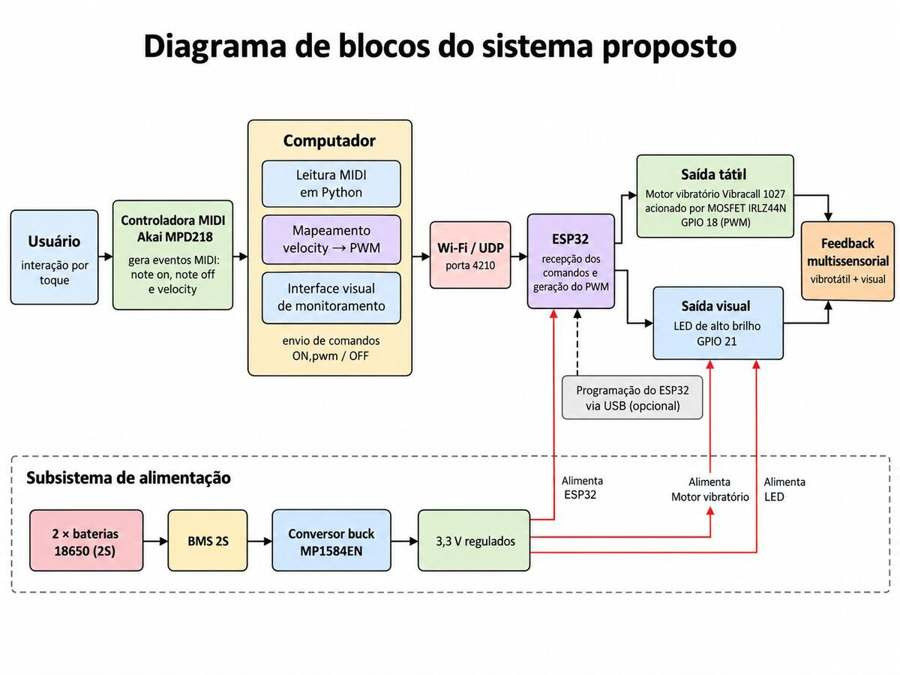
\includegraphics[
width=0.96\linewidth,
keepaspectratio
]{Imagens/Diagramas/diagrama_blocos_sistema.jpg}
\caption{Diagrama de blocos da arquitetura funcional do sistema desenvolvido}
\label{fig:fluxograma_sistema}
\legend{Fonte: Elaboração própria (2026).}
\end{figure}

\section{Interface Musical Digital e Protocolo MIDI}
\markright{Fundamentação Técnica e Arquitetura do Sistema}
\label{sec:interface_midi}

A interface de entrada é baseada no controlador Akai MPD218. O dispositivo converte o acionamento de seus \textit{pads} em mensagens MIDI, disponibilizadas ao computador por USB \cite{akai2015mpd218}.

O protocolo MIDI não transporta o sinal de áudio do instrumento. As mensagens representam eventos da execução, como acionamento e liberação de notas, identificação do elemento acionado e parâmetros de dinâmica \cite{midi1996}. Essa característica permite utilizar informações do gesto antes da geração do som, o que é adequado à proposta de comandar modalidades sensoriais paralelas à saída musical.

\subsection{Controlador MIDI Akai MPD218}
\label{subsec:mpd218}

O MPD218 possui 16 \textit{pads} utilizados como superfície principal de interação. O controlador envia ao computador mensagens que incluem a nota MIDI e o valor de \textit{velocity} associado ao acionamento \cite{akai2015mpd218}. No protótipo, a nota identifica visualmente o \textit{pad} correspondente, enquanto a \textit{velocity} é utilizada no cálculo do nível de controle.

A Figura~\ref{fig:mpd218_esquematico} apresenta uma representação esquemática da disposição dos controles do MPD218.



O controlador não seleciona diferentes motores no sistema desenvolvido. A configuração final utiliza um único atuador vibrotátil, de modo que a identificação da nota permanece vinculada à interface gráfica e ao registro dos eventos.

\begin{figure}[!htbp]
\centering
\resizebox{0.93\linewidth}{!}{\begin{tikzpicture}[x=1cm,y=1cm,scale=0.85,every node/.style={transform shape}]
\draw[rounded corners=0.22cm,fill=black!87,draw=black!50,line width=1.1pt] (0,0) rectangle (13,8.3);
\node[anchor=west,text=white,font=\bfseries\scriptsize] at (0.35,7.88) {AKAI PROFESSIONAL};
\node[anchor=east,text=white,font=\bfseries] at (12.6,7.82) {MPD218};
\foreach \y in {2.85,4.45,6.05}{
 \foreach \x in {0.75,2.25}{
  \shade[ball color=black!40] (\x,\y) circle (0.39);
  \draw[draw=black!15,line width=0.75pt] (\x,\y) circle (0.40);
  \draw[draw=white!70,line width=1pt] (\x,\y) -- ++(0,0.23);
 }
}
\foreach \i in {0,1,2,3}{
 \foreach \j in {0,1,2,3}{
  \pgfmathtruncatemacro{\padnum}{4*\i+\j+1}
  \draw[fill=black!70,draw=red!60!black,line width=1.2pt,rounded corners=0.08cm]
    (3.52+2.18*\j,0.60+1.72*\i) rectangle (5.37+2.18*\j,2.05+1.72*\i);
  \node[anchor=south west,text=white,font=\scriptsize] at (3.62+2.18*\j,0.66+1.72*\i) {\padnum};
 }
}
\foreach \y in {0.90,1.55}{
 \foreach \x in {0.58,1.50,2.42}{
  \draw[fill=black!40,draw=white!50,rounded corners=0.05cm]
    (\x-0.34,\y-0.21) rectangle (\x+0.34,\y+0.21);
 }
}
\node[text=white,font=\tiny,align=left,anchor=west] at (0.28,0.15) {16 pads e 6 potenciômetros};
\end{tikzpicture}
}
\caption{Representação esquemática do controlador Akai MPD218, com 16 \textit{pads} e seis potenciômetros}
\label{fig:mpd218_esquematico}
\legend{Fonte: Elaboração própria, com base em \textcite{akai2015mpd218}.}
\end{figure}

\subsection{Mensagens MIDI e Parâmetro \textit{Velocity}}
\label{subsec:velocity_midi}

Entre as mensagens relevantes para a aplicação estão \textit{note\_on} e \textit{note\_off}. No MIDI 1.0, o campo \textit{velocity} é codificado em sete bits e admite valores de 0 a 127. Um evento \textit{note\_on} com \textit{velocity} igual a zero também pode representar o encerramento da nota \cite{midi1996}.

A \textit{velocity} fornece uma variável digital associada à dinâmica do acionamento. Neste trabalho, seu valor é empregado como entrada para uma função de mapeamento implementada em Python. A saída dessa função é o valor PWM transmitido ao ESP32.

A relação funcional pode ser representada por

\begin{equation}
V_{\mathrm{MIDI}}
\longrightarrow
f(V_{\mathrm{MIDI}})
\longrightarrow
P_{\mathrm{PWM}}
\longrightarrow
\left\{
\begin{array}{l}
\text{feedback vibrotátil}\\
\text{feedback visual}
\end{array}
\right.,
\end{equation}

em que $V_{\mathrm{MIDI}}$ representa a \textit{velocity}, $f(\cdot)$ corresponde ao mapeamento implementado no software e $P_{\mathrm{PWM}}$ é o comando utilizado pelas saídas.

A escolha dessa variável não implica equivalência entre gesto e intensidade percebida. O mapeamento estabelece uma relação de controle; a resposta mecânica do motor, a resposta luminosa do LED e a percepção humana possuem características próprias e são tratadas separadamente nas limitações do trabalho.

\section{Arquitetura do Sistema Proposto}
\markright{Fundamentação Técnica e Arquitetura do Sistema}
\label{sec:arquitetura_sistema}

O sistema pode ser dividido em seis módulos funcionais. A interface musical registra o gesto do usuário; o processamento computacional interpreta as mensagens MIDI e calcula o comando; a comunicação transfere esse comando ao módulo embarcado; o ESP32 gera as saídas; o sistema de alimentação fornece energia localmente; e os elementos de \textit{feedback} convertem o comando em respostas tátil e visual.

Essa organização modular permite alterar individualmente a interface de entrada, a função de mapeamento, o protocolo de comunicação, o atuador ou a forma de alimentação. No protótipo validado, os módulos foram integrados em uma cadeia única, mas permaneceram testáveis de forma independente.

O protocolo UDP opera por datagramas e não fornece, por si só, mecanismos de confirmação de entrega, ordenação ou retransmissão \cite{postel1980udp}. Sua utilização foi escolhida pela simplicidade da troca de mensagens curtas e pela baixa sobrecarga para a aplicação em rede local. A confiabilidade observada no ensaio realizado é discutida no Capítulo 5 e não é generalizada para outras condições de rede.

\section{Unidade de Controle Embarcada}
\markright{Fundamentação Técnica e Arquitetura do Sistema}
\label{sec:esp32}

A unidade de controle embarcada utiliza um módulo ESP32-WROOM-32 instalado em uma placa de desenvolvimento com conector micro-USB. O ESP32 concentra a recepção dos comandos e a geração das saídas do módulo vestível. O dispositivo possui conectividade Wi-Fi integrada e periféricos destinados à geração de sinais PWM, características compatíveis com a arquitetura proposta \cite{espressif2026esp32,espressifledc}.

O processamento musical permanece no computador. O microcontrolador recebe comandos já convertidos para a faixa de controle e não interpreta diretamente o protocolo MIDI. Essa divisão reduz a complexidade do software embarcado e separa o tratamento dos eventos musicais da atuação física.

Após a recepção de um comando válido, o ESP32 atualiza o canal do motor e o canal do LED. O motor não é alimentado diretamente pelo GPIO; o pino controla o MOSFET, enquanto a corrente do atuador é fornecida pelo barramento regulado. O LED, por sua vez, é acionado por uma saída dedicada com resistor limitador de corrente.

\section{Sistema de Feedback Multissensorial}
\markright{Fundamentação Técnica e Arquitetura do Sistema}
\label{sec:feedback_vibrotatil}

As saídas do sistema foram definidas para apresentar a mesma informação de controle por duas modalidades. O motor Vibracall 1027 produz o \textit{feedback} vibrotátil e o LED de alto brilho produz o \textit{feedback} visual.

O mesmo valor PWM é utilizado como referência para as duas saídas, mas essa decisão não estabelece equivalência perceptiva entre elas. Um valor digital comum pode produzir respostas físicas com relações distintas de amplitude, frequência, brilho e percepção. O compartilhamento do comando deve ser entendido apenas como sincronização funcional das modalidades.

A proposta também não reproduz o conteúdo acústico do MIDI. Nota, timbre e frequência sonora não são convertidos diretamente em frequência de vibração ou cor. O sistema representa eventos da interação e sua intensidade relativa, preservando o instante de acionamento e o valor de controle calculado.

\section{Fluxo de Funcionamento Durante a Interação}
\markright{Fundamentação Técnica e Arquitetura do Sistema}
\label{sec:fluxo_funcionamento}

Cada acionamento de um \textit{pad} gera uma mensagem MIDI recebida pelo programa. Para eventos válidos, a nota é utilizada na identificação visual e a \textit{velocity} é convertida para o valor PWM correspondente. O comando é transmitido por UDP ao ESP32, que atualiza o GPIO 18 e o GPIO 21. Dessa forma, o evento produz respostas vibrotátil e visual sincronizadas ao mesmo comando digital.

Quando a liberação do \textit{pad} é identificada, o software transmite \texttt{OFF}, interrompendo as duas saídas. O fluxo funcional pode ser sintetizado por

\begin{equation}
\begin{split}
\text{Gesto}
&\rightarrow
\text{Evento MIDI}
\rightarrow
\textit{Velocity}\\
&\rightarrow
\text{Processamento em Python}
\rightarrow
\text{UDP/Wi-Fi}\\
&\rightarrow
\text{ESP32}
\rightarrow
\text{PWM}
\rightarrow
\begin{cases}
\text{feedback vibrotátil}\\
\text{feedback visual}.
\end{cases}
\end{split}
\end{equation}

A interface gráfica é atualizada em paralelo à transmissão. A unidade vestível permanece alimentada localmente, sem cabo de dados ou alimentação para o computador.

\chapter{Metodologia}

Esta seção apresenta os procedimentos adotados para o desenvolvimento, a implementação e a validação técnica da interface musical multissensorial proposta.

A metodologia foi organizada de forma incremental, iniciando pelo dimensionamento e pela simulação do circuito eletrônico de acionamento, seguida pela implementação da lógica computacional, configuração da comunicação entre o computador e o sistema embarcado e integração progressiva dos diferentes módulos do protótipo.

Após a validação inicial em bancada, foi realizada uma etapa adicional de integração destinada à transformação do circuito experimental em uma unidade vestível com alimentação própria. Nessa etapa foram incorporados o sistema de alimentação por baterias, o estágio de regulação de tensão e o LED de alto brilho utilizado como modalidade física complementar de feedback visual.

Os procedimentos experimentais abrangeram a aquisição das mensagens MIDI, o mapeamento entre o parâmetro \textit{velocity} e os valores PWM, a comunicação UDP, o estágio eletrônico de acionamento, a alimentação embarcada, o funcionamento dos canais tátil e visual e a operação integrada da arquitetura.

Os resultados obtidos a partir desses procedimentos são apresentados e discutidos no Capítulo 5.

\section{Estratégia Geral de Desenvolvimento}
\markright{Metodologia}
\label{sec:estrategia_desenvolvimento}

O desenvolvimento foi organizado em etapas modulares: definição dos requisitos de aquisição MIDI e resposta multissensorial, dimensionamento e simulação do circuito de acionamento, implementação do software e da comunicação UDP, testes de bancada e integração dos módulos em uma unidade vestível.

Os componentes eletrônicos foram avaliados inicialmente de forma independente, com verificação do estágio de chaveamento antes da conexão do motor. Posteriormente foram incorporados o canal visual, a alimentação por baterias e o invólucro. Essa sequência permitiu identificar problemas de montagem antes da operação integrada.

Os ensaios utilizaram registros dos programas Python, do monitor serial do ESP32, arquivos CSV e medições elétricas. Os procedimentos específicos são descritos nas seções seguintes.

\subsection{Componentes de Hardware}
\markright{Metodologia}
\label{sec:componentes_hardware}

A Tabela~\ref{tab:componentes_hardware} reúne os componentes principais da configuração final.

\begin{table}[htbp]
\centering
\caption{Principais componentes de hardware utilizados no sistema}
\label{tab:componentes_hardware}
\footnotesize
\begin{tabular}{|p{2.8cm}|p{2.8cm}|c|p{6.8cm}|}
\hline
\textbf{Componente} &
\textbf{Modelo / especificação} &
\textbf{Qtd.} &
\textbf{Função no sistema} \\
\hline
Controlador MIDI & Akai MPD218 & 1 &
Geração das mensagens MIDI a partir da interação com os \textit{pads}. \\
\hline
Microcontrolador & ESP32-WROOM-32 (placa de desenvolvimento) & 1 &
Recepção dos comandos via Wi-Fi/UDP e controle das saídas. \\
\hline
Motor vibrotátil & Vibracall 1027 & 1 &
Produção do \textit{feedback} vibrotátil. \\
\hline
Transistor MOSFET & IRLZ44N & 1 &
Chaveamento da corrente do motor a partir do sinal de controle. \\
\hline
Diodo de proteção & 1N5819 & 1 &
Recirculação da corrente indutiva durante o desligamento do motor. \\
\hline
Resistor de \textit{gate} & 220~$\Omega$ & 1 &
Limitação da corrente transitória associada ao acionamento do \textit{gate}. \\
\hline
Resistor \textit{pull-down} & 47~k$\Omega$ & 1 &
Manutenção do MOSFET no estado desligado sem comando ativo. \\
\hline
LED de alto brilho & -- & 1 &
Produção do \textit{feedback} visual. \\
\hline
Resistor do LED & 220~$\Omega$ & 1 &
Limitação da corrente no LED. \\
\hline
Baterias recarregáveis & Li-ion 18650, 3,7~V & 2 &
Fornecimento de energia à unidade vestível em configuração 2S. \\
\hline
Sistema de proteção & BMS 2S & 1 &
Proteção do conjunto de baterias. \\
\hline
Conversor DC--DC & MP1584EN & 1 &
Redução e ajuste da tensão para aproximadamente 3,3~V. \\
\hline
Computador & Uso geral & 1 &
Aquisição MIDI, interface gráfica, cálculo do comando e transmissão UDP. \\
\hline
\end{tabular}
\legend{Fonte: Elaboração própria (2026).}
\end{table}

Os componentes foram selecionados para atender às funções de aquisição, processamento, comunicação e atuação com disponibilidade comercial e simplicidade de reprodução. O dimensionamento dos resistores, a escolha do estágio de proteção e a estratégia de alimentação são detalhados na Seção~\ref{sec:dimensionamento_circuito}.

\section{Dimensionamento do Circuito Eletrônico}
\markright{Metodologia}
\label{sec:dimensionamento_circuito}


O circuito eletrônico de acionamento foi dimensionado para permitir o controle do motor vibrotátil a partir do sinal PWM gerado pelo microcontrolador ESP32, evitando que a corrente necessária ao atuador seja fornecida diretamente pelo pino GPIO.

O dimensionamento considerou as limitações das saídas do microcontrolador, o comportamento indutivo do motor de corrente contínua, os transitórios associados ao chaveamento PWM e a necessidade de proteção do estágio eletrônico.

A configuração final utiliza um canal de acionamento vibrotátil baseado em transistor MOSFET de canal N. O canal visual é controlado por uma saída independente do ESP32 e utiliza um LED de alto brilho conectado por meio de resistor limitador de corrente.

Embora as duas modalidades possuam circuitos de saída distintos, o mesmo valor PWM calculado a partir do parâmetro \textit{velocity} é utilizado como referência para o acionamento do motor e do LED.

\subsection{Circuito Eletrônico de Acionamento}
\markright{Metodologia}
\label{sec:implementacao_eletronica}

O estágio vibrotátil foi implementado com um MOSFET IRLZ44N de canal N em configuração \textit{low-side}. O terminal positivo do motor é conectado ao barramento regulado, o terminal negativo ao \textit{drain} do MOSFET e o \textit{source} ao GND. O sinal PWM do GPIO 18 é aplicado ao \textit{gate} por um resistor de 220~$\Omega$, e um resistor de 47~k$\Omega$ mantém o transistor desligado quando o pino de controle não está ativamente polarizado.

O IRLZ44N é classificado pelo fabricante como MOSFET de nível lógico, mas seus valores garantidos de resistência de condução são especificados para tensões de \textit{gate} superiores à alimentação lógica utilizada neste protótipo \cite{infineonirlz44n}. Por essa razão, não se assume saturação plena a 3,3~V. A adequação do componente, nas condições empregadas e com a corrente reduzida do motor, foi incluída nos ensaios de validação funcional.

O motor apresenta comportamento indutivo. Um diodo Schottky 1N5819 foi conectado em paralelo ao atuador, polarizado reversamente durante a condução normal, para fornecer caminho de recirculação à corrente no desligamento \cite{vishay1n5819}. A influência dessa proteção é analisada nas simulações da Seção~\ref{sec:simulacao_circuito}.

O canal visual é eletricamente independente do estágio com MOSFET. O LED de alto brilho é conectado ao GPIO 21 em série com um resistor de 220~$\Omega$. Não foram empregados capacitores de desacoplamento adicionais nem fusível resetável PTC na montagem final descrita nesta monografia.

A Figura~\ref{fig:esquematico_canais_saida} apresenta o esquema elétrico dos canais de saída, incluindo o estágio de acionamento do motor, o diodo de proteção e o canal visual.

\begin{figure}[!htbp]
\centering
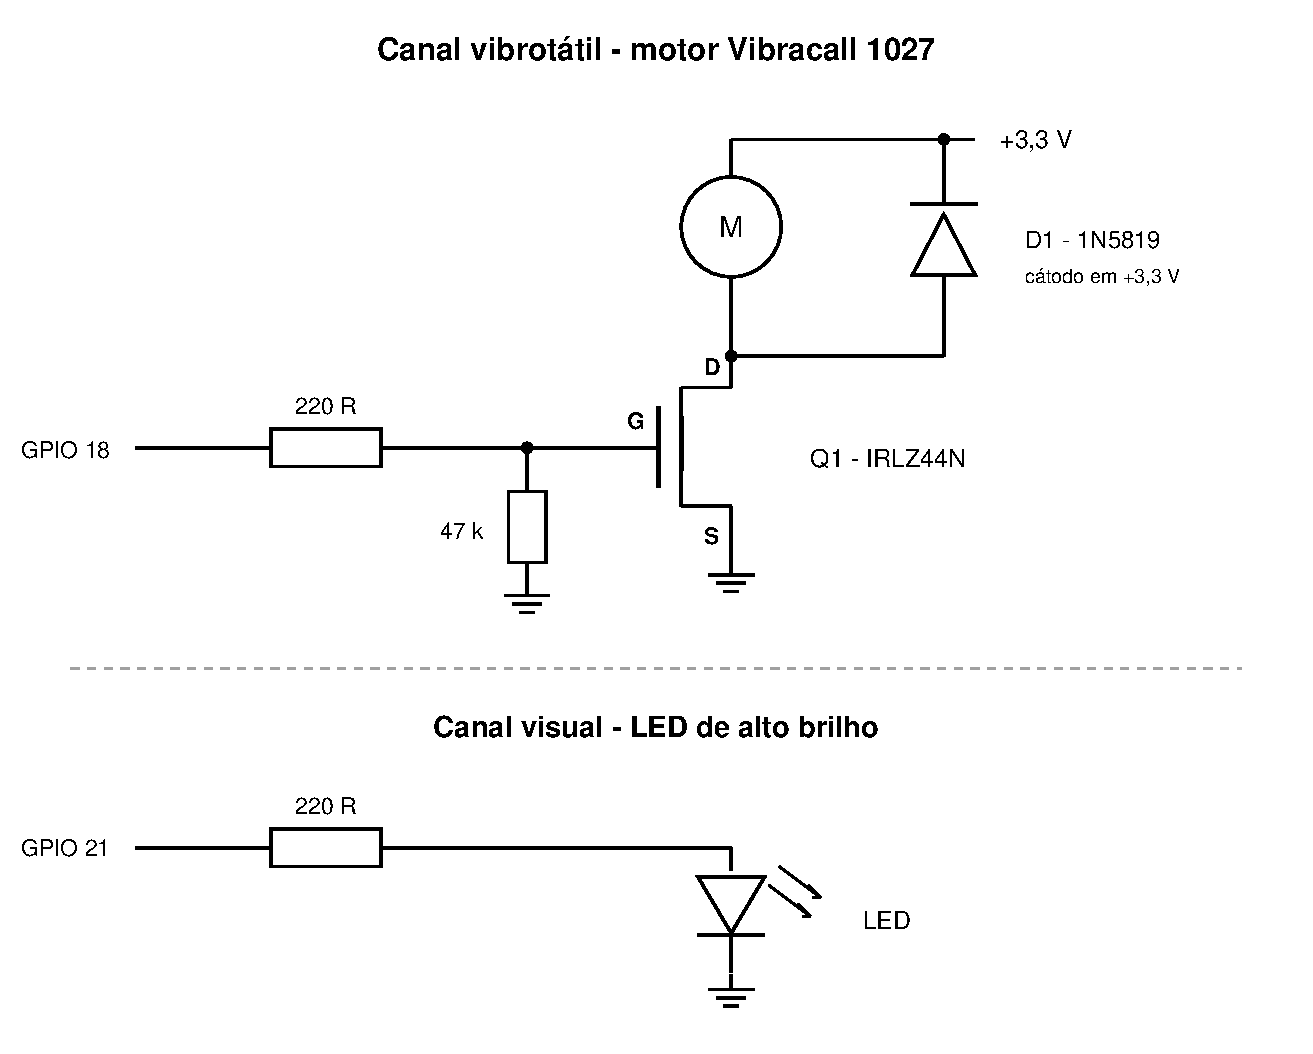
\includegraphics[width=0.90\linewidth,keepaspectratio]{Imagens/Diagramas/circuito_canais_saida.pdf}
\caption{Esquema elétrico dos canais de acionamento vibrotátil e visual}
\label{fig:esquematico_canais_saida}
\legend{Fonte: Elaboração própria (2026).}
\end{figure}

\subsection{Seleção do Transistor MOSFET}
\markright{Metodologia}
\label{sec:selecao_mosfet}


Para o chaveamento do motor vibrotátil foi selecionado o MOSFET IRLZ44N de canal N. O componente é classificado como dispositivo de nível lógico, embora as especificações de resistência de condução do fabricante sejam fornecidas para tensões de gate superiores a 3,3~V \cite{infineonirlz44n}. Por esse motivo, sua utilização foi submetida à avaliação funcional nas condições de corrente do protótipo, sem se assumir saturação plena do transistor na tensão lógica empregada.

O componente foi empregado em configuração \textit{low-side}, na qual o terminal \textit{source} é conectado ao GND do circuito e o terminal \textit{drain} é conectado ao terminal de retorno do motor. O terminal positivo do atuador permanece conectado ao barramento de alimentação.

Essa configuração permite que o sinal PWM gerado pelo ESP32 controle a condução do transistor sem que a corrente necessária ao motor seja fornecida diretamente pelo pino GPIO.

Na configuração final do protótipo foi utilizado um MOSFET IRLZ44N para o canal de acionamento vibrotátil.

\subsection{Resistor de \textit{Gate}}
\markright{Metodologia}
\label{sec:resistor_gate}

Foi utilizado um resistor de 220~$\Omega$ em série entre a saída GPIO do ESP32 responsável pelo controle vibrotátil e o terminal \textit{gate} do MOSFET.

A função desse resistor é limitar as correntes transitórias associadas à carga e descarga da capacitância de entrada do transistor e auxiliar no amortecimento de oscilações durante as transições de chaveamento.

O valor de 220~$\Omega$ foi adotado como compromisso entre a limitação dos transitórios provenientes do GPIO e a manutenção de uma velocidade de chaveamento compatível com o controle PWM empregado no protótipo.

\subsection{Resistor \textit{Pull-Down}}
\markright{Metodologia}
\label{sec:pull_down}


Foi utilizado um resistor \textit{pull-down} de 47~k$\Omega$ conectado entre o terminal \textit{gate} do MOSFET e o GND.

Esse componente mantém o potencial do \textit{gate} próximo de zero quando o pino do microcontrolador se encontra em alta impedância, como pode ocorrer durante a inicialização ou reinicialização do ESP32.

Dessa forma, reduz-se a possibilidade de acionamento involuntário do motor decorrente de um estado elétrico indefinido no terminal de controle do transistor.

O valor de 47~k$\Omega$ foi utilizado por oferecer uma referência definida para o \textit{gate} com baixa corrente estática no circuito de polarização.

\subsection{Proteção contra Transitórios Indutivos}
\markright{Metodologia}
\label{sec:protecao_flyback}


Por apresentar comportamento indutivo, o motor vibrotátil armazena energia durante seu acionamento. Quando a condução do MOSFET é interrompida, a corrente associada à indutância tende a permanecer circulando, podendo produzir transitórios de tensão no estágio de chaveamento.

Para fornecer um caminho de recirculação dessa corrente durante o desligamento, foi utilizado um diodo Schottky 1N5819 conectado em paralelo com o motor e polarizado reversamente durante a operação normal \cite{vishay1n5819}.

O cátodo do diodo foi conectado ao terminal positivo do motor, enquanto o ânodo foi conectado ao terminal associado ao \textit{drain} do MOSFET.

A influência desse elemento de proteção foi posteriormente analisada por meio das simulações elétricas descritas na Seção~\ref{sec:simulacao_flyback}.

\subsection{Estratégia de Alimentação}
\markright{Metodologia}
\label{sec:estrategia_alimentacao}

A estratégia de alimentação do protótipo foi desenvolvida em duas etapas.

Durante a fase inicial de montagem e validação em bancada, o ESP32 foi alimentado por sua interface USB, enquanto o estágio destinado ao motor vibrotátil utilizava uma fonte externa dedicada. Essa configuração facilitou os procedimentos de depuração e permitiu avaliar separadamente os módulos do sistema.

Após a validação funcional da cadeia de controle, foi implementada uma solução de alimentação embarcada com o objetivo de eliminar as conexões físicas entre a estrutura vestível e fontes externas durante a operação.

Para essa configuração foram utilizadas duas células recarregáveis de íons de lítio de 3,7~V associadas em série, formando um conjunto 2S. As células foram associadas a um módulo BMS compatível, destinado à proteção do conjunto.

Como a tensão fornecida pelas baterias é superior à tensão utilizada pelo circuito embarcado, foi empregado um conversor DC--DC baseado no MP1584EN.

O módulo utilizado na montagem é apresentado na Figura~\ref{fig:modulo_mp1584en}. Seu ajuste foi realizado antes da conexão ao restante do circuito, de forma a evitar a aplicação de uma tensão superior à prevista no barramento do sistema embarcado.

\begin{figure}[!htbp]
\centering
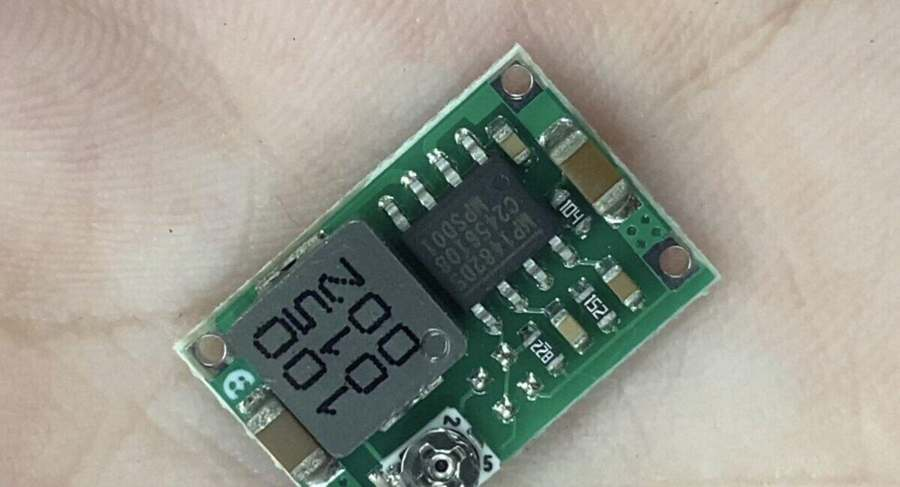
\includegraphics[
width=0.58\linewidth,
keepaspectratio
]{Imagens/Fotos/modulo_mp1584en.jpg}
\caption{Módulo conversor DC--DC utilizado para ajuste da alimentação do circuito embarcado}
\label{fig:modulo_mp1584en}
\legend{Fonte: Elaboração própria (2026).}
\end{figure}


Antes da conexão ao circuito, a saída do conversor foi ajustada com auxílio de multímetro para aproximadamente 3,3~V. Somente após a verificação da tensão de saída o estágio foi conectado ao ESP32 e aos demais elementos da unidade vestível.

Durante os ensaios de integração, a tensão foi monitorada diretamente no barramento de alimentação do microcontrolador enquanto a interface Wi-Fi permanecia ativa. Esse procedimento permitiu verificar o comportamento da alimentação sob uma condição representativa de operação.

O barramento regulado fornece energia ao ESP32 e ao estágio associado ao atuador vibrotátil. Todos os elementos do sistema embarcado compartilham a mesma referência de GND.

A montagem final não utilizou capacitores adicionais de desacoplamento nem fusível resetável PTC. Esses componentes, considerados em etapas preliminares de projeto, não integram a configuração física validada.

A corrente necessária ao motor não é fornecida diretamente pelo GPIO. O pino do ESP32 fornece apenas o sinal PWM aplicado ao \textit{gate} do MOSFET, enquanto a corrente do atuador é proveniente do barramento de alimentação.

Com essa configuração, a unidade vestível passou a operar utilizando alimentação própria, sem necessidade de conexão USB ou de uma fonte externa durante a utilização normal. A comunicação com o computador permanece realizada exclusivamente por Wi-Fi.

O arranjo de alimentação embarcada e sua distribuição funcional são apresentados na Figura~\ref{fig:diagrama_alimentacao_embarcada}. O diagrama representa a organização dos módulos, não o detalhamento dos terminais específicos do BMS.

\begin{figure}[!htbp]
\centering
\resizebox{0.98\linewidth}{!}{\begin{tikzpicture}[
 >=Latex,node distance=5mm and 6mm,
 bloco/.style={draw,rounded corners=3pt,align=center,text width=29mm,minimum height=14mm,font=\small,fill=black!4},
 linha/.style={-Latex,thick}
]
\node[bloco] (bat) {Duas células\\18650 (2S)};
\node[bloco,right=of bat] (bms) {Proteção\\BMS 2S};
\node[bloco,right=of bms] (dc) {Conversor\\MP1584EN};
\node[bloco,right=of dc] (barr) {Barramento\\$+3{,}3$ V / GND};
\draw[linha] (bat) -- (bms);
\draw[linha] (bms) -- (dc);
\draw[linha] (dc) -- (barr);
\node[bloco,below=14mm of barr] (esp) {ESP32-WROOM-32\\alimentação};
\node[bloco,left=of esp] (motor) {Estágio MOSFET\\e motor};
\node[bloco,left=of motor] (led) {LED e resistor\\limitador};
\coordinate (ramo) at ($(barr.south)+(0,-0.35)$);
\draw (barr.south) -- (ramo);
\draw[linha] (ramo) -- (esp.north);
\draw[linha] (ramo) -| (motor.north);
\draw[linha] (ramo) -| (led.north);
\node[font=\scriptsize,below=6mm of motor,align=center] {Os três ramos compartilham\\a referência de GND.};
\end{tikzpicture}
}
\caption{Diagrama funcional do sistema de alimentação embarcada}
\label{fig:diagrama_alimentacao_embarcada}
\legend{Fonte: Elaboração própria (2026).}
\end{figure}


\section{Invólucro e Organização Física do Protótipo}
\markright{Metodologia}
\label{sec:involucro_prototipo}

Após a validação dos módulos eletrônicos em bancada, a montagem foi consolidada em uma placa perfurada, reduzindo o volume ocupado pelas interligações e permitindo acomodar o conjunto em uma estrutura portátil. A Figura~\ref{fig:pci_prototipo} registra as duas faces da placa utilizada no protótipo. Na vista frontal observam-se o ESP32 e os componentes do estágio eletrônico, enquanto a vista posterior evidencia as conexões soldadas responsáveis pela interligação do circuito.

\begin{figure}[!htbp]
\centering
\begin{minipage}[t]{0.47\textwidth}
\centering
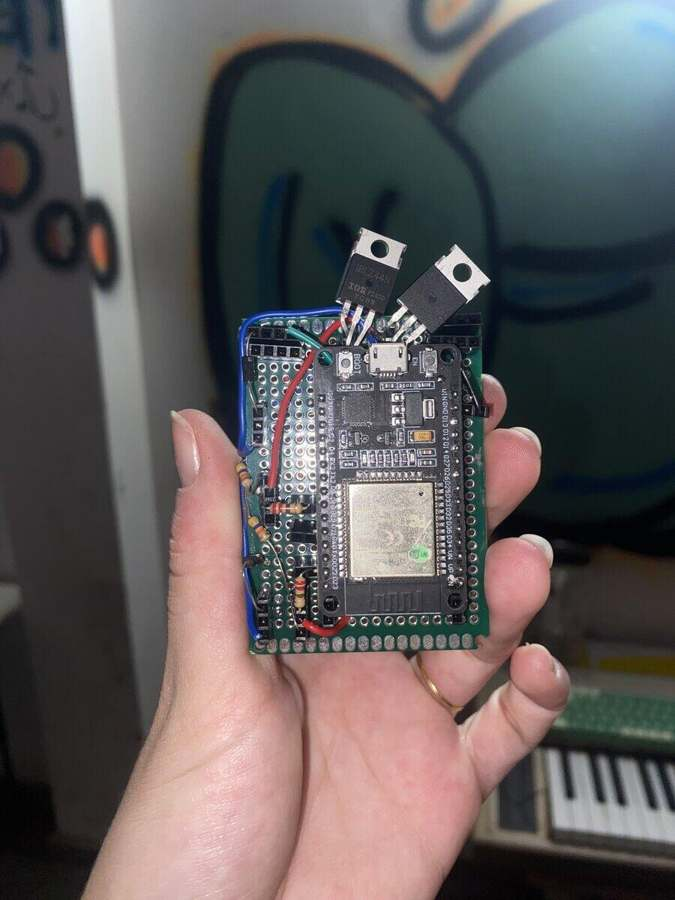
\includegraphics[width=\linewidth]{Imagens/Fotos/pci_frente.jpg}
\end{minipage}
\hfill
\begin{minipage}[t]{0.47\textwidth}
\centering
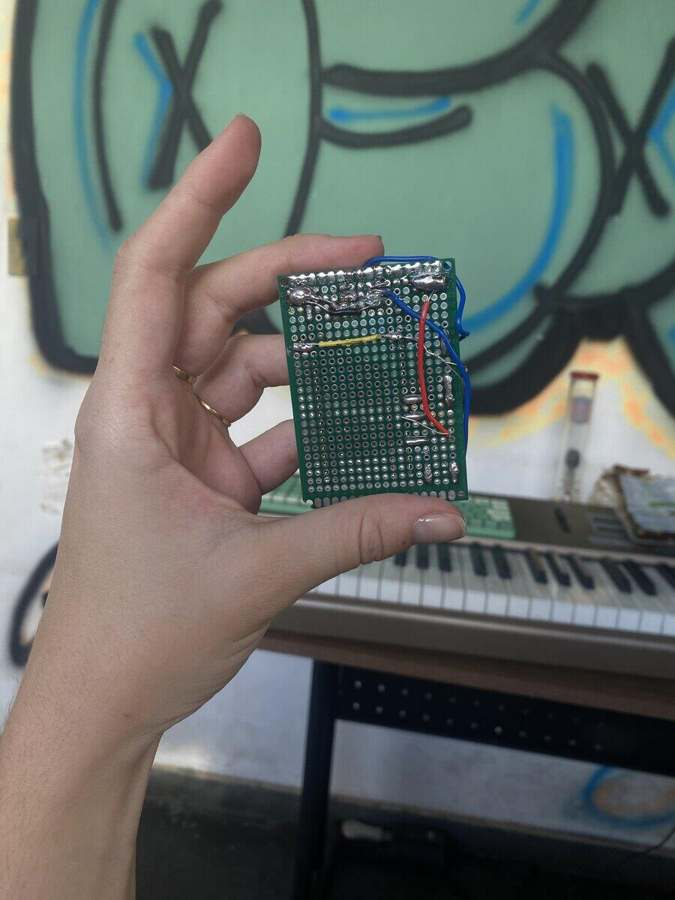
\includegraphics[width=\linewidth]{Imagens/Fotos/pci_verso.jpg}
\end{minipage}
\caption{Montagem do circuito em placa perfurada: vista frontal, à esquerda, e vista posterior, à direita}
\label{fig:pci_prototipo}
\legend{Fonte: Elaboração própria (2026).}
\end{figure}

Com o objetivo de proteger a eletrônica e facilitar sua fixação ao corpo, foi desenvolvido um invólucro específico para a unidade embarcada. O modelo foi dividido em duas peças independentes, constituídas por um corpo principal e uma tampa. Essa separação permitiu manter acesso ao circuito durante as etapas de montagem, depuração e manutenção.

O desenvolvimento do modelo digital contou com apoio do ambiente Cursor \cite{cursor2026}, utilizado como ferramenta auxiliar durante a elaboração e o ajuste da geometria. O uso da ferramenta teve caráter de apoio ao processo de modelagem: as dimensões, a adequação física e as decisões relacionadas à integração dos componentes foram verificadas a partir da montagem real do protótipo.

A geometria final foi exportada em formato STL. O arquivo \texttt{caixa\_corpo.stl} corresponde ao corpo principal do invólucro, enquanto \texttt{caixa\_tampa.stl} corresponde à tampa.

Os arquivos foram preservados como parte do material de reprodução do projeto, permitindo que o invólucro seja fabricado novamente por impressão 3D ou utilizado como ponto de partida para modificações futuras.

A Figura~\ref{fig:modelos_inv_3d} apresenta uma visualização tridimensional dos arquivos STL utilizados no invólucro, com o corpo principal à esquerda e a tampa à direita.

\begin{figure}[!htbp]
\centering
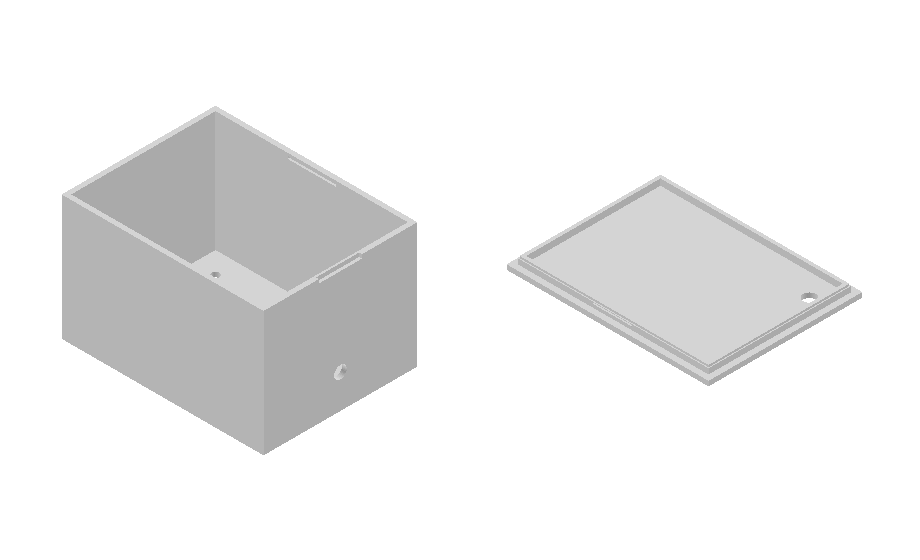
\includegraphics[width=0.95\linewidth,keepaspectratio]{Imagens/Diagramas/modelos_involucro_3d.png}
\caption{Modelos tridimensionais do corpo principal e da tampa do invólucro, renderizados a partir dos arquivos STL do protótipo}
\label{fig:modelos_inv_3d}
\legend{Fonte: Elaboração própria (2026).}
\end{figure}

A Figura~\ref{fig:caixa_motor_led} apresenta detalhes da integração mecânica dos elementos de feedback. Na vista externa, o LED permanece aparente na tampa da caixa, permitindo a observação do canal visual. Na base destinada ao contato com o braço, o motor vibrotátil foi fixado de forma a favorecer a transmissão do estímulo mecânico à região de uso.

\begin{figure}[!htbp]
\centering
\begin{minipage}[t]{0.47\textwidth}
\centering
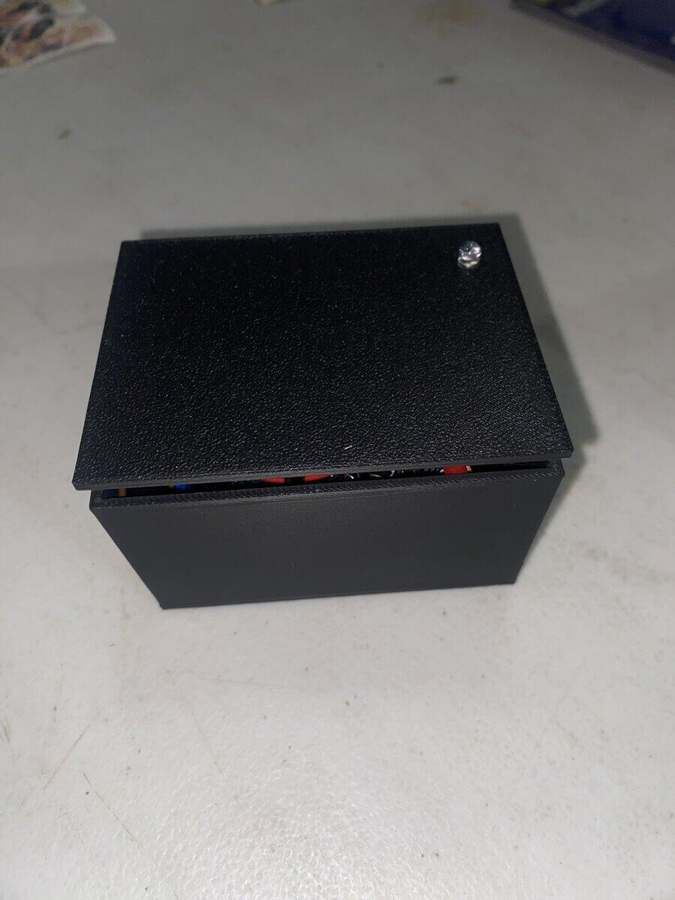
\includegraphics[width=\linewidth]{Imagens/Fotos/caixa_led.jpg}
\end{minipage}
\hfill
\begin{minipage}[t]{0.47\textwidth}
\centering
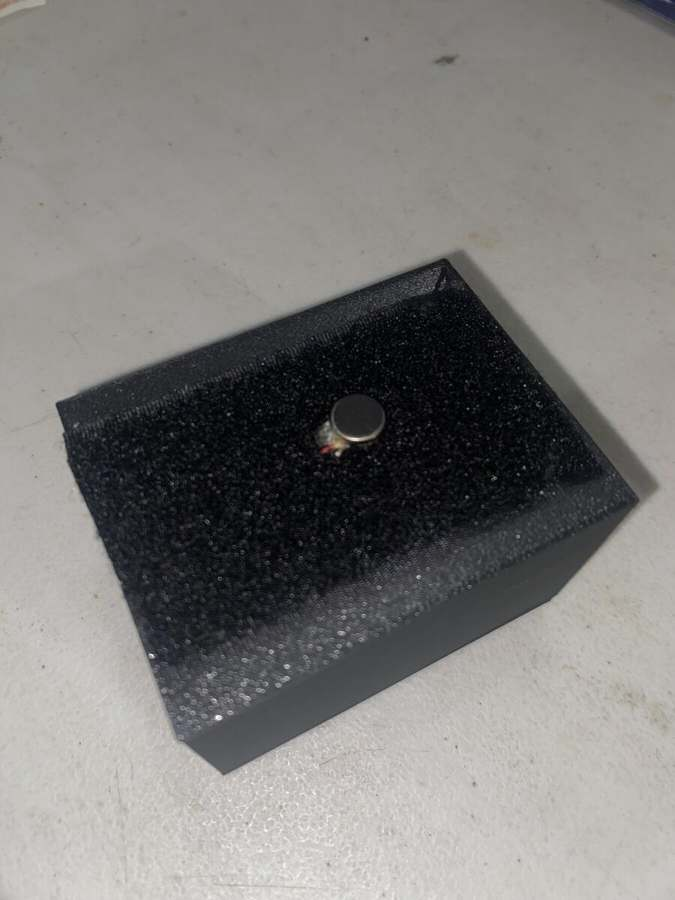
\includegraphics[width=\linewidth]{Imagens/Fotos/fundo_caixa_motor.jpg}
\end{minipage}
\caption{Integração dos elementos de feedback ao invólucro: caixa impressa com o LED aparente, à esquerda, e base com o motor vibrotátil fixado, à direita}
\label{fig:caixa_motor_led}
\legend{Fonte: Elaboração própria (2026).}
\end{figure}

A fixação ao antebraço foi realizada por meio de uma faixa de velcro. A Figura~\ref{fig:elementos_vestiveis} mostra, antes da montagem no usuário, a pulseira e a caixa com o motor posicionado na superfície destinada ao contato com o braço.

\begin{figure}[!htbp]
\centering
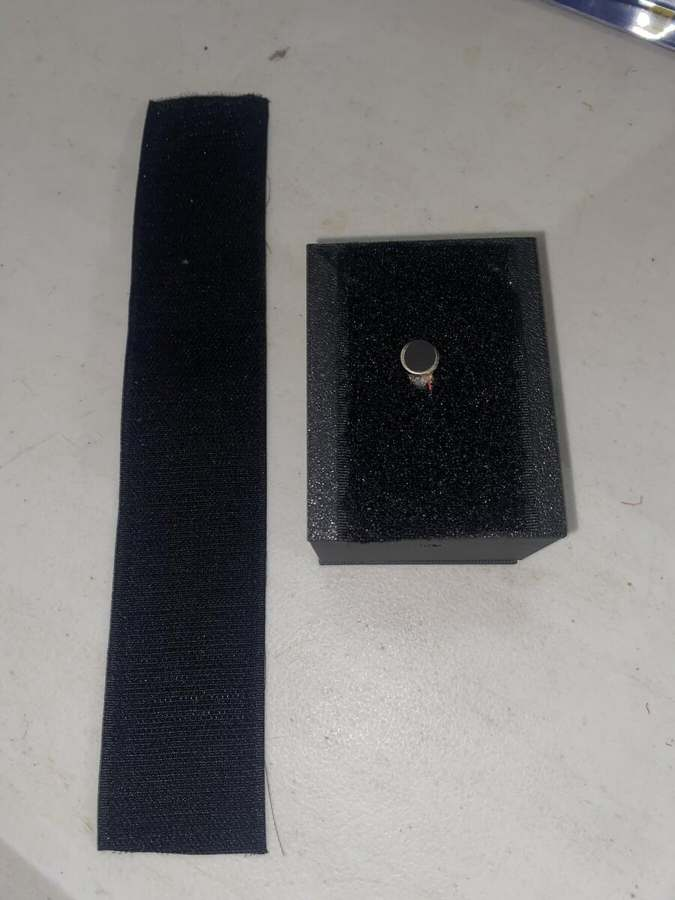
\includegraphics[
width=0.48\linewidth,
keepaspectratio
]{Imagens/Fotos/pulseira_caixa_componentes.jpg}
\caption{Pulseira de velcro e caixa impressa utilizadas na configuração vestível do protótipo}
\label{fig:elementos_vestiveis}
\legend{Fonte: Elaboração própria (2026).}
\end{figure}

A configuração final montada no antebraço é apresentada na Figura~\ref{fig:prototipo_final_vestivel}. As duas vistas registram a disposição da caixa sobre a pulseira e a posição do LED na face superior. A solução deve ser entendida como uma implementação experimental para validação da arquitetura. Não foram conduzidos ensaios formais de ergonomia, conforto prolongado, distribuição de massa, pressão de contato ou posicionamento ótimo do atuador.

\begin{figure}[!htbp]
\centering
\begin{minipage}[t]{0.47\textwidth}
\centering
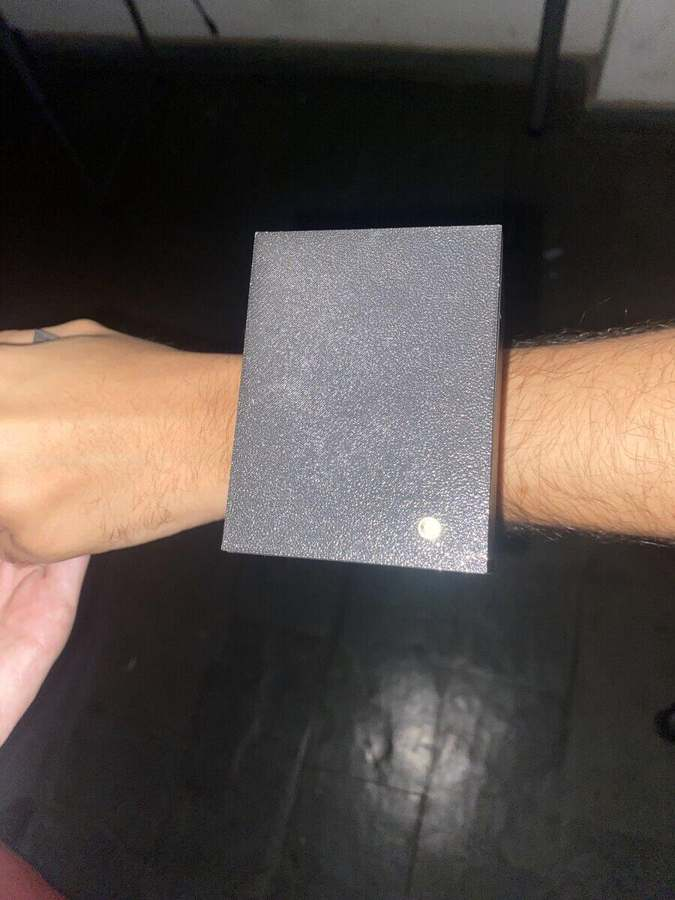
\includegraphics[width=\linewidth]{Imagens/Fotos/prototipo_final_superior.jpg}
\end{minipage}
\hfill
\begin{minipage}[t]{0.47\textwidth}
\centering
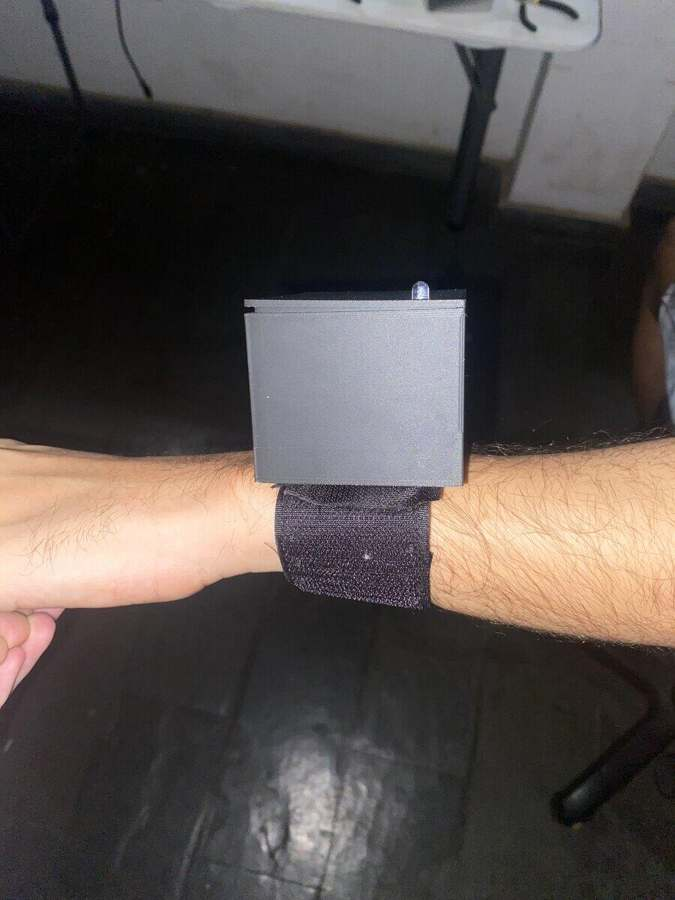
\includegraphics[width=\linewidth]{Imagens/Fotos/prototipo_final_lateral.jpg}
\end{minipage}
\caption{Protótipo final em configuração vestível: vista superior, à esquerda, e vista lateral, à direita}
\label{fig:prototipo_final_vestivel}
\legend{Fonte: Elaboração própria (2026).}
\end{figure}

A documentação pública associada ao trabalho reúne os modelos tridimensionais, instruções de montagem, organização do hardware e arquivos de software necessários à reprodução do sistema.


\section{Simulação do Circuito Eletrônico}
\markright{Metodologia}
\label{sec:simulacao_circuito}

Antes da integração física completa do circuito de acionamento, foram realizadas simulações elétricas utilizando o software LTspice.

Essa etapa teve como objetivo analisar previamente o comportamento do estágio eletrônico responsável pelo acionamento do motor vibrotátil em condições representativas de operação.

As simulações foram realizadas considerando um único canal de acionamento, correspondente à topologia posteriormente implementada no protótipo físico.

Foram investigados dois aspectos principais: a atuação do diodo de \textit{flyback} durante o desligamento da carga indutiva e o comportamento do circuito para diferentes valores de \textit{duty cycle} do sinal PWM.

Os resultados obtidos a partir dessas simulações são apresentados e discutidos no Capítulo 5.

\subsection{Modelo Elétrico Utilizado}
\markright{Metodologia}
\label{sec:modelo_eletrico_simulacao}

O modelo utilizado no LTspice representa o estágio eletrônico empregado para o acionamento do motor vibrotátil.

O circuito simulado é constituído por uma fonte de alimentação de 3,3~V, um modelo simplificado do motor vibrotátil baseado em uma associação resistiva-indutiva, um transistor MOSFET de canal N em configuração \textit{low-side}, resistor de gate, resistor \textit{pull-down} e diodo de \textit{flyback}.

A representação resistiva-indutiva foi utilizada como aproximação do comportamento elétrico de um motor de corrente contínua durante as análises transitórias.

O modelo não busca reproduzir integralmente o comportamento eletromecânico do Vibracall 1027, mas possibilitar a avaliação qualitativa dos fenômenos elétricos associados ao chaveamento de uma carga indutiva.

O MOSFET foi comandado por um sinal pulsado representativo do PWM produzido pelo ESP32.

Durante as diferentes análises, foram mantidas as características gerais da topologia, alterando-se apenas os parâmetros necessários para cada cenário de simulação.


A Figura~\ref{fig:simulacao_circuito_base} apresenta uma configuração exploratória do circuito-base utilizado nas análises. A imagem inclui componentes auxiliares de simulação, como capacitores e resistência de alimentação, que não foram incorporados à montagem final do protótipo.

\begin{figure}[!htbp]
\centering
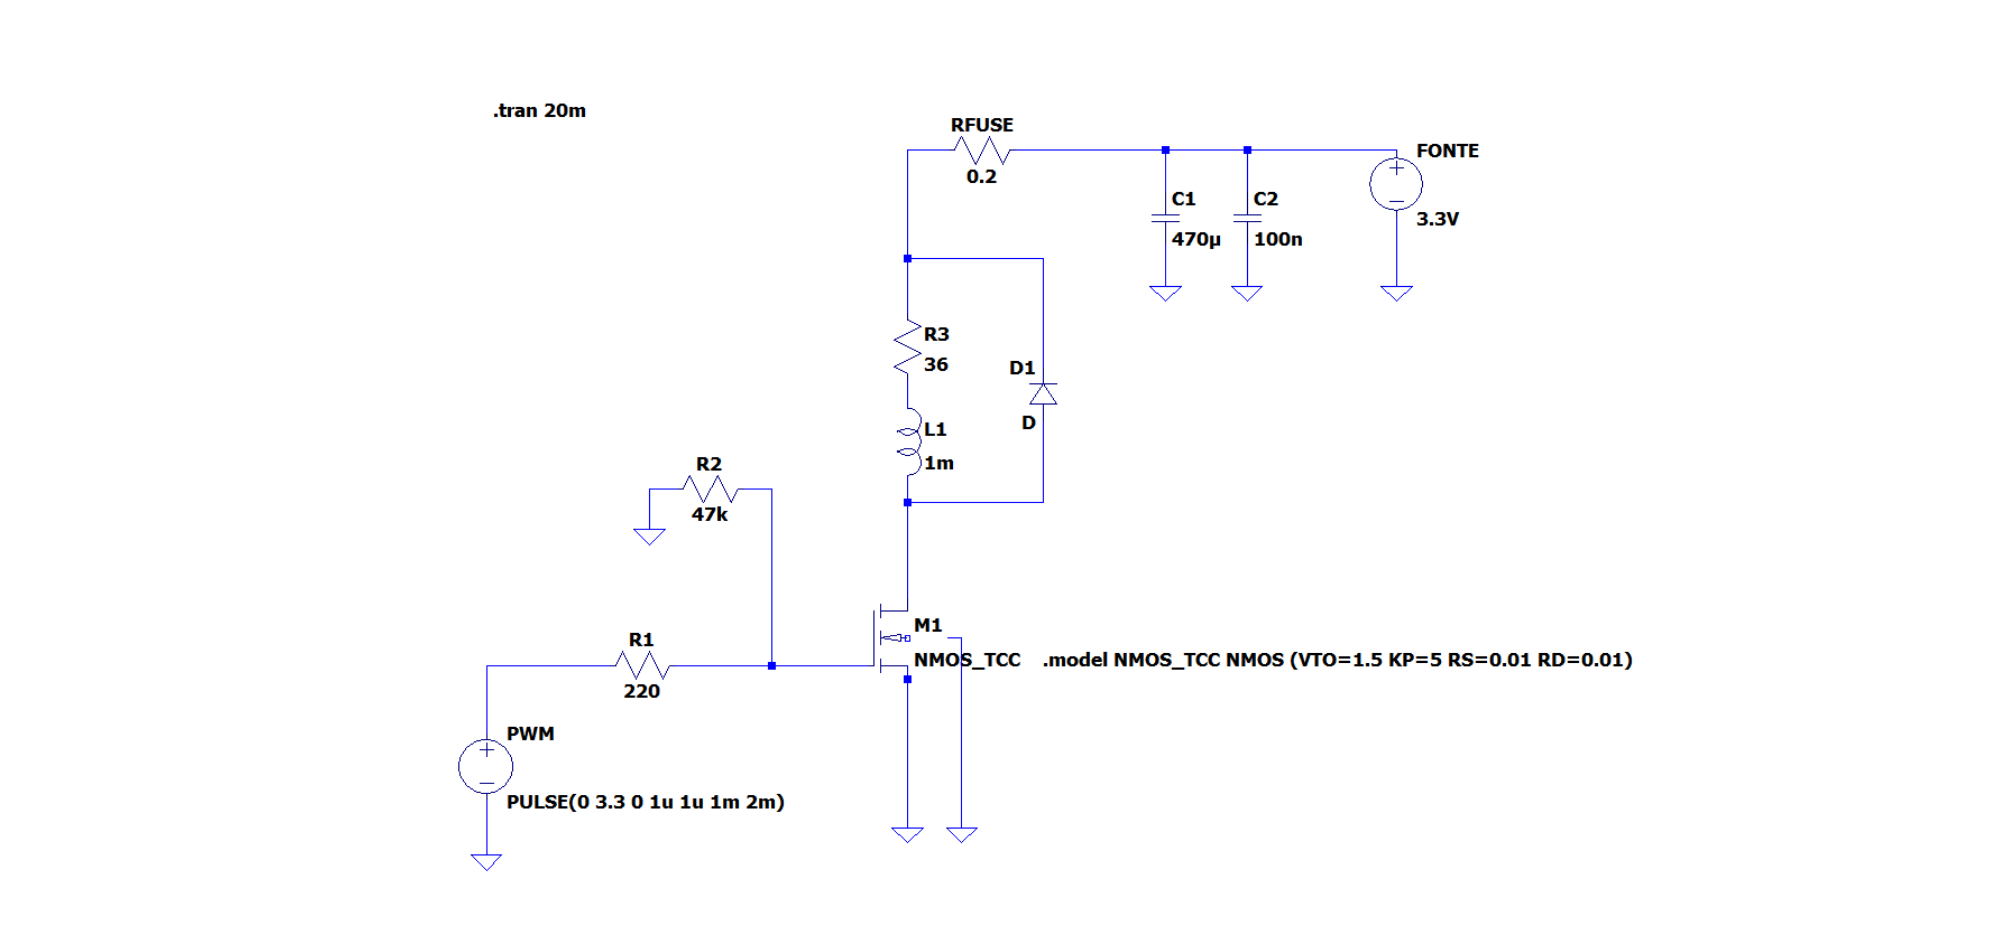
\includegraphics[
width=0.52\linewidth,
trim=240bp 50bp 235bp 35bp,
clip,
keepaspectratio
]{Metodologia/simulacao_circuito_base.png}
\caption{Circuito-base exploratório do acionamento vibrotátil modelado no LTspice}
\label{fig:simulacao_circuito_base}
\legend{Fonte: Elaboração própria (2026).}
\end{figure}

\subsection{Simulação da Proteção por Diodo de \textit{Flyback}}
\markright{Metodologia}
\label{sec:simulacao_flyback}

A influência do diodo de \textit{flyback} foi analisada por meio da comparação entre duas configurações do mesmo estágio eletrônico de acionamento.

Na primeira configuração, foi mantido o diodo Schottky 1N5819 conectado em paralelo com a carga indutiva e polarizado reversamente durante a operação normal.

Na segunda configuração, o componente foi removido do circuito.

Para ambas as condições foram mantidos os demais parâmetros da simulação, permitindo comparar o comportamento transitório produzido durante a interrupção da condução do MOSFET.

A análise foi direcionada principalmente ao comportamento da tensão no estágio de chaveamento e da corrente associada à carga indutiva após a interrupção da condução.

Essa comparação foi utilizada para verificar qualitativamente a função do caminho de recirculação de corrente proporcionado pelo diodo.

As formas de onda obtidas nas configurações com e sem o diodo de \textit{flyback} são apresentadas e discutidas no Capítulo 5.

\subsection{Simulação do Controle PWM}
\markright{Metodologia}
\label{sec:simulacao_pwm}

Para avaliar o comportamento do estágio eletrônico diante de diferentes níveis de comando PWM, foram realizadas simulações mantendo constante a frequência de chaveamento e variando o \textit{duty cycle} do sinal aplicado ao MOSFET.

Foram considerados três níveis de operação:

20\%, 50\% e 80\%.

Para cada condição foram registradas as formas de onda associadas ao acionamento da carga equivalente.

A utilização de diferentes razões cíclicas permitiu comparar o comportamento elétrico do modelo diante de condições de acionamento reduzido, intermediário e elevado.

Essa etapa teve como objetivo verificar qualitativamente se a variação do \textit{duty cycle} produz alterações correspondentes na energia média fornecida à carga equivalente.

Os resultados obtidos para os três níveis de \textit{duty cycle} são apresentados e comparados no Capítulo 5.

\section{Comunicação entre Computador e ESP32}
\markright{Metodologia}
\label{sec:comunicacao_udp}

A comunicação entre o computador responsável pelo processamento das mensagens MIDI e o microcontrolador ESP32 foi implementada por meio do protocolo UDP sobre uma rede Wi-Fi local.

O software desenvolvido em Python é responsável por gerar e transmitir os comandos de controle, enquanto o ESP32 permanece associado à mesma rede e monitora uma porta UDP previamente configurada para receber as mensagens enviadas pelo computador.

Após a recepção de cada comando, o microcontrolador realiza sua interpretação e atualiza as saídas PWM utilizadas pelo sistema.

A utilização do protocolo UDP foi adotada devido à simplicidade da troca de datagramas entre os módulos e à ausência da necessidade de estabelecimento prévio de uma conexão entre o computador e o microcontrolador.

O UDP fornece um mecanismo mínimo de transporte de datagramas e não incorpora mecanismos próprios de confirmação de entrega ou retransmissão \cite{postel1980udp}.

Por esse motivo, foi incluído na metodologia um procedimento específico para avaliar o comportamento da comunicação durante transmissões sucessivas.

\subsection{Formato das Mensagens de Comunicação}
\markright{Metodologia}
\label{sec:formato_mensagens_udp}

Durante a operação normal do sistema, os comandos enviados pelo software em Python informam ao ESP32 o estado de acionamento e, quando aplicável, o valor PWM correspondente.

Para o acionamento das saídas foi utilizado o formato:

\begin{center}
\texttt{ON,valor\_pwm}
\end{center}

em que \texttt{valor\_pwm} representa o nível de controle calculado a partir do parâmetro \textit{velocity} da mensagem MIDI.

Para interromper o acionamento foi utilizado o comando:

\begin{center}
\texttt{OFF}
\end{center}

Após a interpretação da mensagem, o ESP32 aplica o valor PWM recebido ao canal vibrotátil e ao canal visual.

Na configuração implementada, o GPIO 18 controla o estágio de acionamento do motor Vibracall 1027, enquanto o GPIO 21 controla o LED de alto brilho.

Para os ensaios específicos de estabilidade da comunicação, o formato das mensagens foi ampliado com a inclusão de um identificador sequencial de pacote, permitindo comparar os registros de transmissão e recepção.

Nesse caso, os pacotes de teste foram enviados no formato:

\begin{center}
\texttt{ON,id,pwm}
\end{center}

Nesse formato, \texttt{ON} identifica o comando de acionamento, \texttt{id} corresponde ao número sequencial do pacote e \texttt{pwm} representa o valor de controle transmitido ao ESP32.

\subsection{Procedimento de Teste da Comunicação UDP}
\markright{Metodologia}
\label{sec:teste_estabilidade_udp}

Com o objetivo de avaliar o comportamento da comunicação durante transmissões sucessivas, foi implementado um ensaio baseado no envio automatizado de uma sequência de pacotes UDP entre o computador e o ESP32.

O procedimento foi configurado para transmitir 100 pacotes de teste numerados sequencialmente.

Antes do início da sequência utilizada para análise, foi transmitida uma mensagem identificada como \texttt{PING}, empregada como etapa preliminar de inicialização da comunicação.

Os pacotes foram enviados com intervalo aproximado de 50~ms entre transmissões consecutivas.

No computador, o software em Python registrou o identificador de cada pacote, o comando transmitido e o instante relativo de envio.

No ESP32, o monitor serial foi utilizado para registrar os identificadores dos pacotes recebidos e os respectivos instantes relativos de recepção, obtidos a partir da função \texttt{millis()}.

Após a execução do ensaio, os registros produzidos nos dois módulos foram comparados quanto à quantidade de pacotes transmitidos e recebidos, à correspondência entre os identificadores e à regularidade temporal da sequência.

O teste foi utilizado como procedimento de avaliação da estabilidade da comunicação entre os módulos.

Os registros experimentais, a quantidade de pacotes efetivamente recebidos e a análise dos dados temporais são apresentados no Capítulo 5.

\section{Implementação Computacional}
\markright{Metodologia}
\label{sec:implementacao_computacional}

A implementação em Python concentrou no computador a aquisição e o processamento MIDI, o cálculo PWM, a interface gráfica e a preparação dos comandos. O ESP32 recebeu esses comandos para controlar as saídas físicas, permitindo ensaiar separadamente o software e o módulo embarcado.

\subsection{Processamento Computacional e Software}
\markright{Metodologia}
\label{sec:processamento_software}

O software em Python estabelece a ligação entre o controlador MIDI e o módulo embarcado. As bibliotecas \textit{mido} e \textit{python-rtmidi} são utilizadas para acessar a interface MIDI conectada ao computador. A comunicação UDP é implementada por meio de \textit{sockets}.

Durante a execução, o programa monitora as mensagens do MPD218, identifica eventos de acionamento e liberação, obtém a nota e a \textit{velocity} e aplica a função de mapeamento definida para o sistema. O valor calculado atualiza a interface gráfica e compõe o comando transmitido ao ESP32. No encerramento do evento, o software envia o comando de desligamento.

A interface gráfica apresenta os 16 \textit{pads} do controlador e exibe o \textit{pad} acionado, a nota MIDI, a \textit{velocity} e o valor PWM calculado. Essa visualização é um recurso de monitoramento e demonstração no computador; o LED incorporado à unidade vestível constitui a saída visual física destinada ao usuário.

A Figura~\ref{fig:fluxograma_algoritmo} representa o fluxo de processamento dos eventos MIDI, incluindo o filtro temporal, o cálculo do PWM e os comandos transmitidos ao ESP32. A operação descrita corresponde ao programa principal de controle, distinto do mapeamento específico empregado no ensaio de queda.

\begin{figure}[!htbp]
\centering
\resizebox{0.95\linewidth}{!}{\begin{tikzpicture}[
 >=Latex,node distance=6mm and 7mm,
 caixa/.style={draw,rounded corners=2pt,align=center,font=\footnotesize,minimum height=8mm,text width=35mm,fill=black!3},
 decisao/.style={diamond,aspect=2.15,draw,align=center,font=\footnotesize,inner sep=1pt,text width=27mm,fill=black!3},
 seta/.style={-Latex,thick},
 nota/.style={font=\scriptsize,fill=white,inner sep=1pt}
]
\node[caixa] (midi) {Evento MIDI do MPD218};
\node[decisao,below=10mm of midi] (on) {\texttt{note\_on} e \textit{velocity} $>0$?};
\node[decisao,below left=12mm and 20mm of on] (off) {\texttt{note\_off} ou \textit{velocity} $=0$?};
\node[decisao,below right=12mm and 20mm of on] (db) {Intervalo $\geq 0{,}08$ s?};
\node[caixa,below=12mm of off] (sendoff) {Enviar \texttt{OFF} por UDP};
\node[caixa,below=12mm of db] (map) {Calcular PWM proporcional; limitar a 80--255};
\node[caixa,below=7mm of map] (sendon) {Atualizar interface e CSV; enviar \texttt{ON,PWM}};
\node[caixa,below=14mm of sendoff] (zero) {ESP32 aplica PWM 0 ao motor e LED};
\node[caixa,below=7mm of sendon] (motor) {ESP32 aplica PWM aos GPIO 18 e 21};
\draw[seta] (midi) -- (on);
\draw[seta] (on) -| node[nota,pos=.22] {Não} (off);
\draw[seta] (on) -| node[nota,pos=.22] {Sim} (db);
\draw[seta] (off) -- node[nota] {Sim} (sendoff);
\draw[seta] (db) -- node[nota] {Sim} (map);
\draw[seta] (sendoff) -- (zero);
\draw[seta] (map) -- (sendon);
\draw[seta] (sendon) -- (motor);
\node[nota,below=1mm of zero] {Ambas as saídas desligadas};
\node[nota,below=1mm of motor] {Resposta vibrotátil e visual};
\draw[seta] (off.west) -- ++(-9mm,0) node[nota,anchor=east] {Não: ignorar};
\draw[seta] (db.east) -- ++(9mm,0) node[nota,anchor=west] {Não: ignorar};
\end{tikzpicture}
}
\caption{Fluxograma do processamento de eventos MIDI e geração dos comandos de atuação}
\label{fig:fluxograma_algoritmo}
\legend{Fonte: Elaboração própria (2026).}
\end{figure}

\subsection{Aquisição e Tratamento dos Eventos MIDI}
\markright{Metodologia}
\label{sec:aquisicao_midi}

A aquisição das mensagens MIDI foi realizada a partir do controlador Akai MPD218 conectado ao computador por meio de interface USB (Akai Professional, 2015).

No ambiente Python, foram utilizadas as bibliotecas \textit{mido} e \textit{python-rtmidi} para acesso à interface MIDI e leitura das mensagens produzidas durante a interação com os pads.

O software identifica os eventos associados ao acionamento e ao encerramento da interação.

Para os eventos válidos de acionamento, são extraídos o número da nota MIDI e o valor de \textit{velocity}.

O número da nota é utilizado na interface gráfica para identificar o pad correspondente, enquanto o valor de \textit{velocity} é utilizado como variável de entrada para o cálculo do nível de controle.

O número da nota MIDI não é utilizado para selecionar individualmente o atuador vibrotátil.

Na estratégia implementada, o valor PWM calculado a partir da \textit{velocity} é utilizado como referência tanto para o canal vibrotátil quanto para o canal visual.

Os eventos associados ao encerramento do acionamento são utilizados para gerar o comando responsável pela interrupção das duas saídas.

\subsection{Tratamento Temporal dos Eventos MIDI}
\markright{Metodologia}
\label{sec:debounce_midi}

Durante os testes iniciais de aquisição MIDI, foram identificados eventos consecutivos registrados em intervalos temporais reduzidos durante a interação com os pads do controlador.

Com o objetivo de evitar que eventos sucessivos dentro de um intervalo mínimo fossem interpretados como novos acionamentos válidos, foi implementado no software um mecanismo de filtragem temporal.

A estratégia adotada consiste em comparar o instante de cada novo evento com o instante do último evento aceito pelo sistema. Um novo acionamento somente é processado quando o intervalo transcorrido é superior ao limite definido para o filtro.

Durante o desenvolvimento, foi utilizado um intervalo de aproximadamente 80~ms.

A condição de filtragem pode ser representada por:

\begin{equation}
t_{\mathrm{atual}} - t_{\mathrm{ultimo}} < t_{\mathrm{filtro}},
\label{eq:filtro_temporal_midi}
\end{equation}

em que $t_{\mathrm{atual}}$ representa o instante do evento recebido, $t_{\mathrm{ultimo}}$ o instante do último evento considerado válido e $t_{\mathrm{filtro}}$ o intervalo mínimo adotado para a filtragem temporal.

Quando a condição apresentada é satisfeita, o novo evento é desconsiderado para fins de acionamento. Caso contrário, ele é processado normalmente e seu instante passa a ser utilizado como nova referência temporal.

A implementação dessa lógica foi realizada utilizando recursos de medição de tempo disponíveis no ambiente Python.

\subsection{Registro dos Dados Computacionais}
\markright{Metodologia}
\label{sec:registro_dados_computacionais}

Durante os procedimentos de desenvolvimento e validação, o software foi configurado para registrar informações associadas aos eventos processados.

Os registros foram armazenados em arquivos CSV contendo, conforme o ensaio realizado, informações como número da nota MIDI, valor de \textit{velocity} e valor PWM calculado.

Além dos arquivos estruturados, os terminais utilizados durante a execução do software permitiram acompanhar os comandos transmitidos ao sistema embarcado.

Esses registros foram utilizados posteriormente para analisar o comportamento do algoritmo e elaborar os gráficos apresentados no Capítulo 5.


\section{Estratégia de Controle Multissensorial}
\markright{Metodologia}
\label{sec:estrategia_controle}

A estratégia de controle converte o parâmetro \textit{velocity} do evento MIDI em um comando PWM calculado no computador. O ESP32 aplica o nível recebido ao motor conectado ao estágio MOSFET (GPIO 18) e ao LED (GPIO 21). As saídas compartilham a referência digital, sem pressupor equivalência entre intensidade de vibração, brilho e percepção do usuário.

\subsection{Mapeamento entre \textit{Velocity} MIDI e PWM}
\markright{Metodologia}
\label{sec:mapeamento_velocity_pwm}

O parâmetro \textit{velocity} foi utilizado como variável de entrada para determinar o valor de controle aplicado às modalidades de feedback.

Durante a implementação, foi adotado um mapeamento proporcional entre os valores de \textit{velocity} registrados pelo controlador MIDI e a faixa de PWM definida para o sistema.

O algoritmo implementado considera como referência superior o valor de \textit{velocity} igual a 30. Para valores até esse limite, o comando PWM é calculado proporcionalmente por:

\begin{equation}
P_{\mathrm{PWM}} =
\frac{V_{\mathrm{MIDI}}}{30}
\cdot 255
\end{equation}

em que $V_{\mathrm{MIDI}}$ representa o valor de \textit{velocity} recebido e $P_{\mathrm{PWM}}$ representa o valor PWM calculado.

Após o cálculo, é aplicado um limite inferior de 80 aos eventos válidos de acionamento. Dessa forma, valores calculados abaixo desse limite são ajustados para 80.

Valores de \textit{velocity} superiores à referência utilizada produzem valores calculados acima da faixa PWM disponível e são saturados em 255.

A lógica pode ser representada por:

\begin{equation}
P_{\mathrm{PWM}} =
\min
\left(
255,
\max
\left(
80,
\frac{V_{\mathrm{MIDI}}}{30}\cdot255
\right)
\right)
\end{equation}

para eventos de acionamento com \textit{velocity} maior que zero.

O cálculo é realizado no software em Python antes da transmissão ao ESP32.

Na configuração final, o valor resultante é utilizado como referência simultaneamente para o canal vibrotátil e para o canal visual.

Para análise do comportamento do algoritmo, os pares formados pelos valores de \textit{velocity} e pelos respectivos valores PWM calculados foram registrados durante os ensaios.


\subsection{Intervalo de Operação PWM}
\markright{Metodologia}
\label{sec:intervalo_operacao_pwm}

Para o controle dos atuadores foi utilizada uma faixa de PWM compreendida entre 80 e 255 para os eventos válidos de acionamento.

O valor 255 corresponde ao limite superior utilizado na representação PWM adotada na implementação. Valores calculados acima desse limite são saturados em 255.

O valor inferior de 80 foi adotado durante o desenvolvimento para evitar a utilização de comandos muito reduzidos, associados a uma região de acionamento pouco útil para os motores no protótipo experimental.

Assim, para um evento MIDI válido, o comando produzido pelo software permanece limitado ao intervalo:

\begin{equation}
80 \leq P_{\mathrm{PWM}} \leq 255,
\label{eq:intervalo_pwm}
\end{equation}

em que $P_{\mathrm{PWM}}$ representa o valor de controle posteriormente aplicado pelo ESP32 aos canais vibrotátil e visual.

A definição dessa faixa foi utilizada como parâmetro de implementação do protótipo. Sua adequação é discutida no Capítulo 5 a partir dos ensaios realizados com o sistema.

\subsection{Tratamento dos Comandos de Acionamento}
\markright{Metodologia}
\label{sec:comandos_acionamento}

Os formatos \texttt{ON,valor\_pwm} e \texttt{OFF} estão especificados na Seção~\ref{sec:formato_mensagens_udp}. O software envia o comando de acionamento para eventos válidos do tipo \texttt{note\_on} com \textit{velocity} maior que zero. Eventos \texttt{note\_off} e mensagens \texttt{note\_on} com \textit{velocity} igual a zero são tratados como encerramento da nota \cite{midi1996}.

Ao receber \texttt{ON}, o ESP32 atualiza as saídas PWM associadas ao motor e ao LED. O comando \texttt{OFF} atribui valor zero às duas saídas. Assim, a duração de cada resposta acompanha os eventos de acionamento e liberação enviados pelo controlador.


\section{Procedimentos Experimentais de Validação}
\markright{Metodologia}
\label{sec:procedimentos_experimentais}

Os procedimentos experimentais foram definidos com o objetivo de validar progressivamente os diferentes módulos da arquitetura desenvolvida e, posteriormente, verificar seu funcionamento integrado.

A estratégia adotada foi incremental. Inicialmente foram avaliados os sinais de controle e o estágio eletrônico responsável pelo acionamento do motor vibrotátil. Em seguida, foi realizada a validação física do atuador, da comunicação entre o computador e o ESP32 e da alimentação embarcada.

Após a validação do canal vibrotátil, foi incorporado o LED de alto brilho utilizado como modalidade física de feedback visual.

Por fim, foi avaliada a operação simultânea das duas modalidades de saída durante a interação com o controlador MIDI, utilizando a cadeia completa formada pelo Akai MPD218, software em Python, comunicação UDP sobre Wi-Fi, ESP32, motor vibrotátil e LED.

Essa sequência permitiu identificar e corrigir falhas individualmente antes da integração completa do protótipo e reduzir os riscos associados à energização simultânea dos diferentes módulos.


\subsection{Validação do Estágio de Chaveamento}
\markright{Metodologia}
\label{sec:validacao_chaveamento}


Antes da conexão do motor vibrotátil, foi realizada uma validação preliminar do estágio eletrônico utilizando um LED como carga auxiliar de teste.

O ensaio foi conduzido com uma saída GPIO do ESP32 conectada ao terminal \textit{gate} do MOSFET IRLZ44N por meio do resistor de 220~$\Omega$, mantendo também o resistor \textit{pull-down} previsto no circuito.

Foram aplicados diferentes estados de acionamento com o objetivo de verificar o caminho de controle entre o ESP32, o MOSFET e a carga antes da utilização do motor.

Nessa etapa, o LED foi utilizado exclusivamente como ferramenta de depuração do circuito eletrônico, não correspondendo ainda ao canal visual posteriormente incorporado à arquitetura final.


\subsection{Validação de um Canal Vibrotátil}
\markright{Metodologia}
\label{sec:validacao_um_canal}

Após a verificação inicial do estágio eletrônico, foi realizada a validação física utilizando um motor Vibracall 1027 conectado ao circuito de acionamento.

A montagem foi composta pelo ESP32, transistor MOSFET IRLZ44N, resistor de gate, resistor \textit{pull-down}, diodo de \textit{flyback} e motor vibrotátil.

Inicialmente foram realizados testes de continuidade e medições de tensão nos diferentes pontos do circuito com o objetivo de verificar a propagação do sinal de controle entre o GPIO do ESP32 e o terminal \textit{gate} do MOSFET.

Em seguida, comandos transmitidos por UDP foram utilizados para verificar o acionamento e o desligamento do motor.

Posteriormente, o controlador Akai MPD218 foi utilizado para produzir eventos MIDI com diferentes valores de \textit{velocity}. O software desenvolvido em Python processou esses eventos, calculou os valores PWM correspondentes e transmitiu os comandos ao ESP32.


\subsection{Ensaio com Corpo de Massa Conhecida}
\markright{Metodologia}
\label{sec:ensaio_queda_controlada}

Após a validação funcional do canal vibrotátil, foi realizado um ensaio específico para investigar a correspondência entre uma condição mecânica de entrada controlada, o valor de \textit{velocity} fornecido pelo MPD218 e o comando PWM calculado pelo software.

Antes da definição do procedimento definitivo, foi realizado um ensaio exploratório de carregamento estático sobre um dos pads. Nessa montagem, massas foram acrescentadas progressivamente até a ocorrência de acionamento, conforme ilustrado na Figura~\ref{fig:ensaio_estatico_exploratorio}. Esse procedimento foi utilizado apenas como referência preliminar de sensibilidade do pad. Como o parâmetro \textit{velocity} é determinado pelo comportamento dinâmico do acionamento e não por uma carga estática isolada, o ensaio foi mantido apenas como registro exploratório e não integrou a análise quantitativa principal.

\begin{figure}[!htbp]
\centering
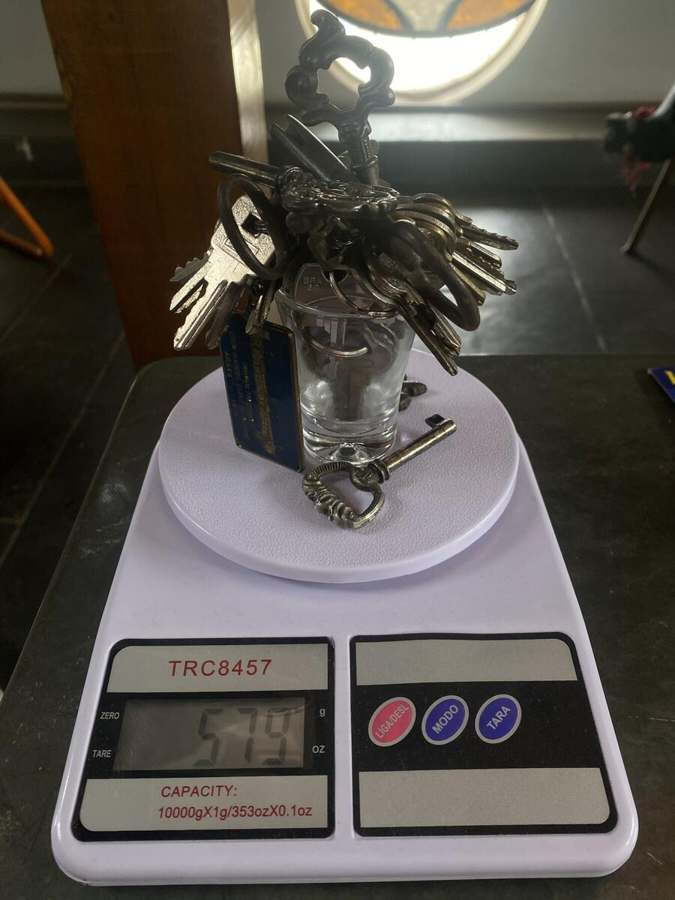
\includegraphics[
width=0.50\linewidth,
keepaspectratio
]{Imagens/Fotos/ensaio_estatico_limiar_pad.jpg}
\caption{Ensaio exploratório de carregamento estático empregado na definição do procedimento experimental}
\label{fig:ensaio_estatico_exploratorio}
\legend{Fonte: Elaboração própria (2026).}
\end{figure}


Foi utilizado um corpo com massa de 39~g, solto sobre o pad 4 do controlador, correspondente à nota MIDI 71. A altura de queda foi medida com régua e variada entre 0,5~cm e 5~cm, nas condições de 0,5; 1; 2; 3; 4 e 5~cm. Para cada altura foram realizadas dez repetições, totalizando 60 quedas independentes. O corpo foi liberado sem impulso adicional, procurando-se manter a região de impacto sobre o mesmo pad.

A Figura~\ref{fig:ensaio_queda_massa} documenta o corpo utilizado e a configuração adotada para controle da altura. A massa foi conferida em balança antes da coleta, e uma régua foi utilizada como referência para posicionar o corpo antes de cada liberação.

\begin{figure}[!htbp]
\centering
\begin{minipage}[t]{0.43\textwidth}
\centering
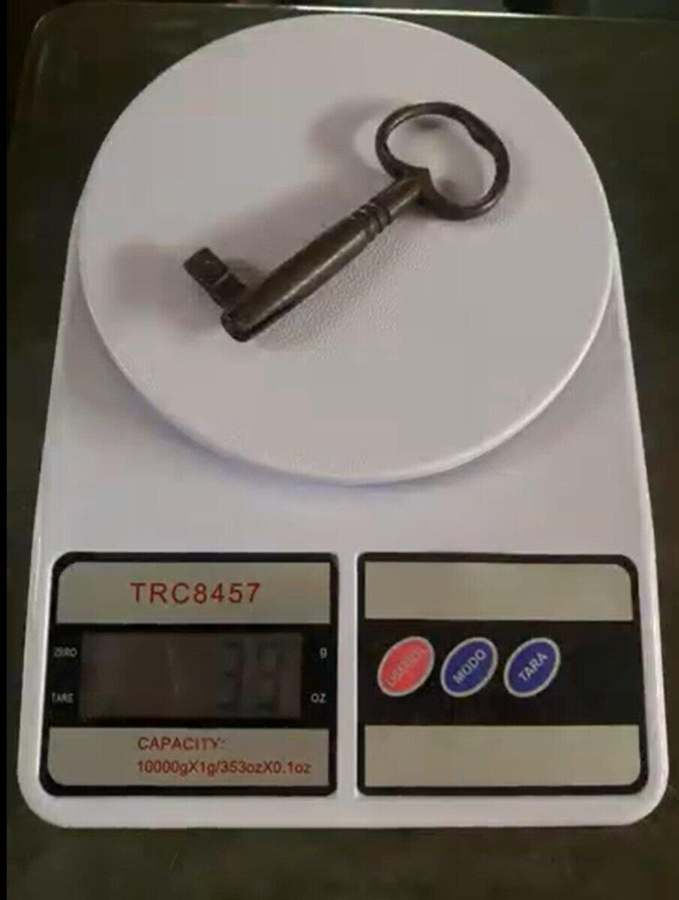
\includegraphics[width=\linewidth]{Imagens/Fotos/massa_39g.jpg}
\end{minipage}
\hfill
\begin{minipage}[t]{0.43\textwidth}
\centering
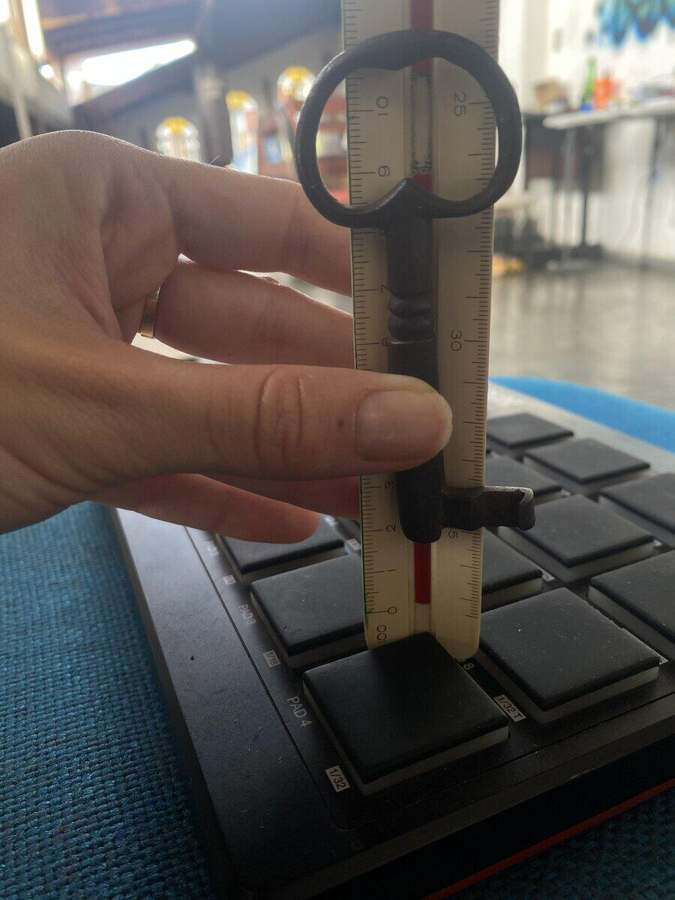
\includegraphics[width=\linewidth]{Imagens/Fotos/ensaio_queda_39g.jpg}
\end{minipage}
\caption{Ensaio com corpo de massa conhecida: aferição da massa de 39~g, à esquerda, e posicionamento do corpo em relação ao pad e à régua de referência, à direita}
\label{fig:ensaio_queda_massa}
\legend{Fonte: Elaboração própria (2026).}
\end{figure}


A escolha dessa faixa foi precedida por ensaios exploratórios, a partir dos quais a faixa utilizada na coleta definitiva foi limitada a 5~cm.

Mantendo-se constante a massa do corpo, a altura de queda foi utilizada como variável de controle da energia potencial gravitacional imediatamente antes da liberação. Para cada condição foram calculadas a energia potencial e a velocidade teórica de impacto, desconsiderando perdas por resistência do ar, por meio de

\begin{equation}
E_p = mgh
\end{equation}

e

\begin{equation}
v = \sqrt{2gh},
\end{equation}

em que $m$ representa a massa do corpo, $g$ a aceleração da gravidade e $h$ a altura de queda. Essas grandezas foram empregadas apenas para caracterizar as condições do ensaio. A força de impacto não foi calculada, pois depende também do tempo e das condições de contato entre o corpo e o pad.

Para este ensaio específico, o programa de aquisição utilizou um mapeamento linear entre a faixa útil de \textit{velocity} MIDI, de 1 a 127, e a faixa de PWM de 80 a 255. Essa escolha permitiu explorar a faixa dinâmica completa do controlador durante a caracterização. O mapeamento empregado no programa de teste foi definido por

\begin{equation}
P_{\mathrm{PWM}} =
80 +
\frac{V_{\mathrm{MIDI}}-1}{126}
\left(255-80\right),
\label{eq:mapeamento_ensaio_queda}
\end{equation}

para $1 \leq V_{\mathrm{MIDI}} \leq 127$, com arredondamento para o valor inteiro mais próximo.

\subsubsection{Filtragem dos repiques}
\label{sec:filtragem_repiques}

Eventos secundários produzidos por repiques após o primeiro contato do corpo com o pad não representam novas quedas independentes e poderiam introduzir repetições artificiais na série experimental.

Para evitar esse efeito, cada repetição foi iniciada manualmente no programa antes da liberação do corpo. Ao ser armada uma nova repetição, os eventos MIDI pendentes eram descartados e o software passava a aguardar o primeiro evento \texttt{note\_on} válido proveniente do pad selecionado. Esse primeiro evento era registrado como impacto principal.

Após o registro, foi aberta uma janela temporal de 0,60~s. Eventos adicionais do mesmo pad ocorridos nesse intervalo foram classificados como repiques e desconsiderados na determinação da \textit{velocity} e do PWM da repetição. A quantidade de eventos descartados permaneceu registrada no arquivo CSV, permitindo verificar posteriormente a ocorrência do fenômeno sem incorporá-lo como uma nova observação experimental.

Ao final da coleta foram calculados, para cada altura, média, mediana, desvio-padrão, valores mínimo e máximo de \textit{velocity} e PWM. A associação entre a altura de queda e a resposta do controlador foi avaliada principalmente pelo coeficiente de correlação de Spearman, adequado à verificação de uma tendência monotônica sem exigir linearidade estrita entre as variáveis.


\subsection{Ensaio Acústico do Atuador em Função do PWM}
\markright{Metodologia}
\label{sec:ensaio_acustico_pwm}

Foi realizado um segundo ensaio com o objetivo de verificar se a alteração do comando PWM produzia mudanças mensuráveis na frequência associada ao funcionamento do motor Vibracall 1027.

O ESP32 foi comandado diretamente por UDP utilizando seis valores de PWM: 80, 115, 150, 185, 220 e 255. Cada condição permaneceu ativa durante 8~s, seguida por um intervalo de 2~s com o motor desligado. A sequência completa foi repetida três vezes, resultando em 18 blocos de acionamento.

A automatização do ensaio permitiu registrar em arquivo CSV os instantes de início e término de cada bloco, possibilitando relacionar posteriormente os trechos da gravação ao valor PWM correspondente. O som produzido durante o funcionamento do atuador foi registrado com um microfone condensador em arquivo WAV, com taxa de amostragem de 44,1~kHz e resolução de 24~bits.

A configuração física utilizada durante a gravação é apresentada na Figura~\ref{fig:ensaio_microfone_condensador}. O motor e o microfone foram mantidos em posições fixas durante a sequência, de modo a reduzir alterações de distância e orientação entre os níveis de PWM avaliados.

\begin{figure}[!htbp]
\centering
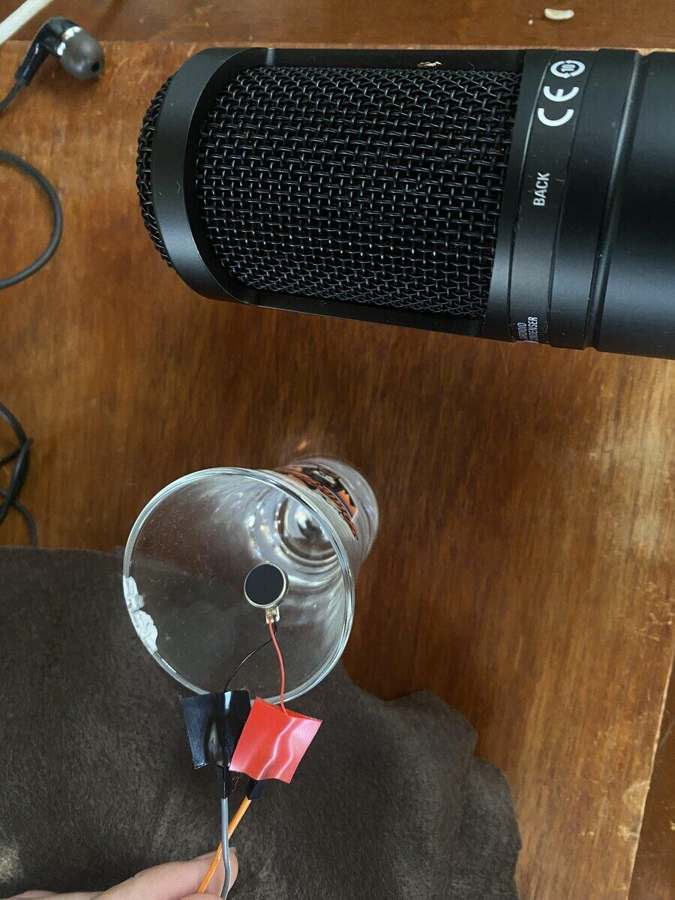
\includegraphics[
width=0.55\linewidth,
keepaspectratio
]{Imagens/Fotos/ensaio_microfone.jpg}
\caption{Configuração experimental utilizada na caracterização acústica do motor com microfone condensador}
\label{fig:ensaio_microfone_condensador}
\legend{Fonte: Elaboração própria (2026).}
\end{figure}


A análise foi realizada no domínio da frequência. Para cada bloco de acionamento foi considerada a região de funcionamento estabelecido do motor, evitando-se as transições de partida e desligamento. A componente tonal de baixa frequência associada ao atuador foi então identificada no espectro de cada trecho. Componentes estacionárias que não acompanharam a variação do PWM foram desconsideradas na determinação da frequência representativa do motor.

Foram calculadas a média, o desvio-padrão e o coeficiente de variação das três repetições para cada valor PWM. Também foram determinados os coeficientes de correlação de Pearson e de Spearman entre o comando aplicado e a frequência acústica identificada.

Esse procedimento fornece uma medida indireta do comportamento dinâmico do motor. Como a grandeza foi obtida por captação acústica, os valores não correspondem a uma medição direta da aceleração, do deslocamento ou da amplitude mecânica da vibração.


\subsection{Validação da Alimentação Embarcada}

Após a validação do circuito utilizando alimentação de bancada, foi realizada a integração do sistema de alimentação destinado à operação autônoma da unidade vestível.

Foram utilizadas duas células recarregáveis de íons de lítio associadas em configuração 2S, juntamente com um módulo BMS e um conversor DC--DC baseado no MP1584EN.

Antes da conexão ao ESP32, a tensão de saída do conversor foi ajustada utilizando multímetro para um valor próximo de 3,3~V.

Após a conexão do circuito embarcado, foram realizadas medições diretamente no barramento de alimentação do ESP32 durante sua operação.

Também foram realizados testes de conectividade entre o computador e o ESP32 utilizando mensagens ICMP por meio do comando \texttt{ping}. Esses testes foram empregados como verificação auxiliar da permanência do microcontrolador conectado à rede durante a operação alimentada pelas baterias.

\subsection{Validação do Feedback Visual}

Após a validação do canal vibrotátil e da alimentação embarcada, foi incorporado ao protótipo um LED de alto brilho destinado à geração do feedback visual.

O LED foi conectado ao GPIO 21 do ESP32 por meio de um resistor de 220~$\Omega$, utilizado para limitar a corrente fornecida ao componente.

O firmware do microcontrolador foi modificado para aplicar ao LED o mesmo valor PWM recebido para o controle do canal vibrotátil.

Inicialmente, o funcionamento do canal visual foi avaliado por meio do envio direto de comandos UDP.

Posteriormente, foram utilizados valores PWM diferentes para verificar a capacidade de modificar o nível de acionamento do LED a partir do mesmo parâmetro utilizado para o controle vibrotátil.


\subsection{Validação Integrada da Arquitetura}

A etapa final dos procedimentos experimentais consistiu na operação integrada dos principais módulos da arquitetura desenvolvida.

O ensaio foi realizado utilizando a cadeia formada pelo controlador MIDI Akai MPD218, computador com o software desenvolvido em Python, comunicação UDP sobre rede Wi-Fi, microcontrolador ESP32, estágio eletrônico de acionamento, motor Vibracall 1027, LED de alto brilho e sistema de alimentação embarcado.

Durante a interação com os pads, os eventos MIDI foram capturados pelo software e seus respectivos valores de \textit{velocity} foram processados para determinação do comando PWM.

Os comandos foram transmitidos ao ESP32, que aplicou o mesmo valor de controle ao canal vibrotátil associado ao GPIO 18 e ao canal visual associado ao GPIO 21.

Também foi utilizada a interface gráfica desenvolvida no computador para acompanhar os eventos MIDI, o pad acionado, o valor de \textit{velocity} e o valor PWM calculado durante a execução.

Os resultados obtidos durante esses procedimentos são apresentados e discutidos no Capítulo 5.

\section{Critérios de Validação}
\markright{Metodologia}
\label{sec:criterios_validacao}

A validação considerou o funcionamento individual dos módulos e sua integração. Na aquisição MIDI, verificou-se a identificação de eventos e a extração da \textit{velocity}; no processamento, a relação monotônica entre valores crescentes de entrada e comandos PWM, respeitados os limites mínimo e máximo definidos. Para a comunicação UDP, foram comparados os identificadores e as quantidades de pacotes transmitidos e recebidos, além de seus registros temporais.

A avaliação eletrônica considerou a capacidade do ESP32 de comandar o MOSFET e o motor, bem como a resposta do LED aos comandos de acionamento, desligamento e variação de PWM. Na alimentação, verificou-se a operação do microcontrolador conectado à rede Wi-Fi utilizando baterias, BMS e conversor DC--DC, sem alimentação USB. A validação integrada exigiu a propagação de um evento MIDI até as saídas vibrotátil e visual, com a unidade embarcada alimentada localmente.

No ensaio de queda, a evidência de resposta foi a tendência monotônica entre altura e \textit{velocity}, considerando a dispersão dos registros e excluindo repiques conforme o procedimento estabelecido. No ensaio acústico, foram comparadas as frequências identificadas para níveis crescentes de PWM, com suas variações entre repetições. As simulações elétricas foram examinadas separadamente, pela resposta do modelo com e sem diodo de \textit{flyback} e para diferentes razões cíclicas.

Esses critérios avaliam a viabilidade técnica, não a equivalência perceptiva das modalidades. Os resultados são discutidos no Capítulo 5.

\chapter{Resultados e Discussão}

Esta seção apresenta os resultados obtidos a partir dos procedimentos de validação descritos no Capítulo 4 e discute seu significado no contexto da arquitetura desenvolvida.

Os resultados são organizados de acordo com os principais módulos avaliados: simulações elétricas do circuito de acionamento, implementação computacional, comunicação UDP, validação física do canal vibrotátil, ensaio com estímulo mecânico controlado, caracterização acústica do atuador, alimentação embarcada, feedback visual e operação integrada do sistema.

A análise concentra-se nos aspectos técnicos e funcionais do protótipo, considerando a aquisição dos eventos MIDI, o processamento do parâmetro \textit{velocity}, o mapeamento para os comandos PWM, a transmissão das mensagens ao ESP32 e a geração simultânea dos feedbacks vibrotátil e visual.

Como o trabalho não contempla ensaios clínicos nem estudos formais de percepção com participantes, as discussões apresentadas nesta seção permanecem restritas aos resultados técnicos, computacionais, elétricos e funcionais observados durante os experimentos.


\section{Resultados das Simulações Elétricas}
\markright{Resultados e Discussão}
\label{sec:resultados_simulacoes_eletricas}

As simulações descritas na Seção~\ref{sec:simulacao_circuito} foram utilizadas para avaliar qualitativamente o comportamento do estágio eletrônico de acionamento antes da integração física completa do protótipo.

A análise considerou dois aspectos principais: a influência do diodo de \textit{flyback} durante o chaveamento da carga indutiva e o comportamento do circuito diante de diferentes valores de \textit{duty cycle} do sinal PWM.

Os resultados apresentados nesta seção devem ser interpretados como uma análise do comportamento elétrico do modelo equivalente utilizado no LTspice, não correspondendo a uma caracterização completa do comportamento eletromecânico do motor Vibracall 1027.


\subsection{Proteção por Diodo de \textit{Flyback}}
\markright{Resultados e Discussão}
\label{sec:resultado_flyback}

A Figura~\ref{fig:simulacao_com_flyback} apresenta a resposta transitória do circuito utilizando o diodo de \textit{flyback} em paralelo com a carga indutiva equivalente.

\begin{figure}[!htbp]
\centering
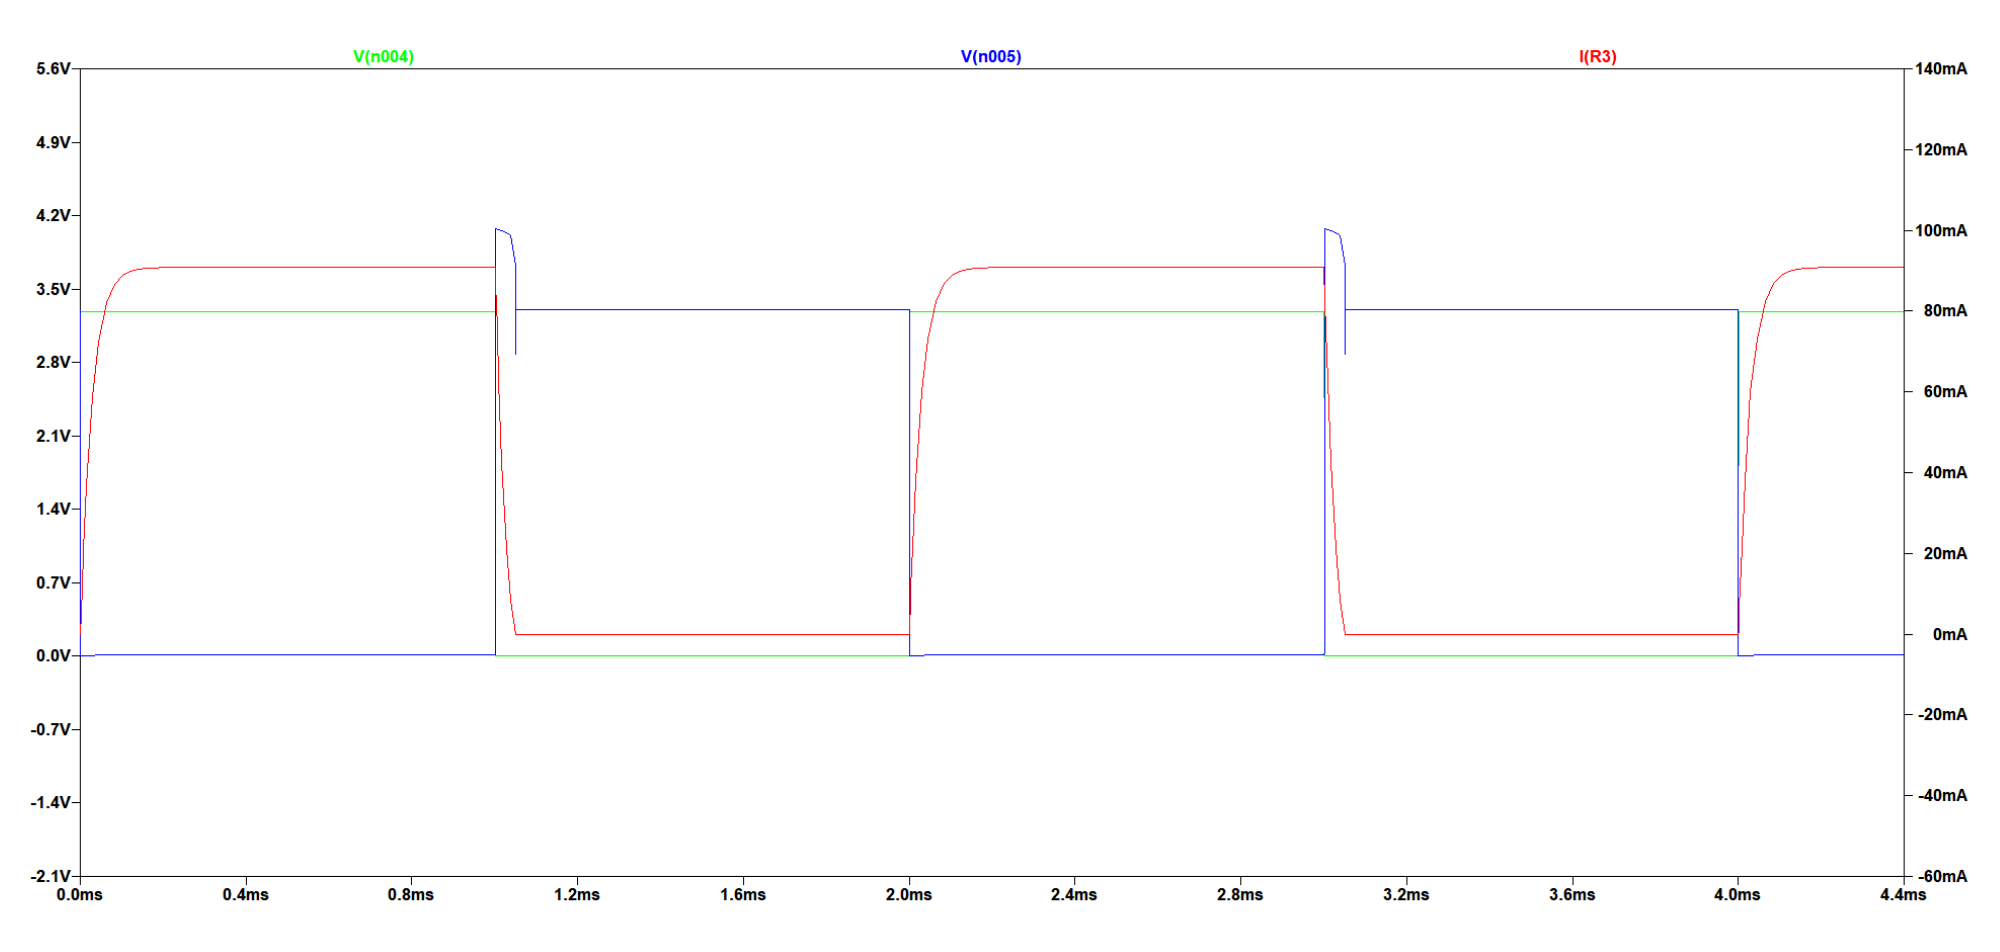
\includegraphics[
width=0.95\linewidth,
keepaspectratio
]{Metodologia/simulacao_com_flyback.png}
\caption{Resposta transitória do circuito utilizando diodo de \textit{flyback}}
\label{fig:simulacao_com_flyback}
\legend{Fonte: Elaboração própria (2026).}
\end{figure}

Na condição simulada com o diodo, os transitórios de tensão associados à interrupção da corrente na carga indutiva foram limitados pela existência de um caminho de recirculação de corrente.

A Figura~\ref{fig:simulacao_sem_flyback} apresenta o comportamento do mesmo circuito na ausência do diodo de proteção.

\begin{figure}[!htbp]
\centering
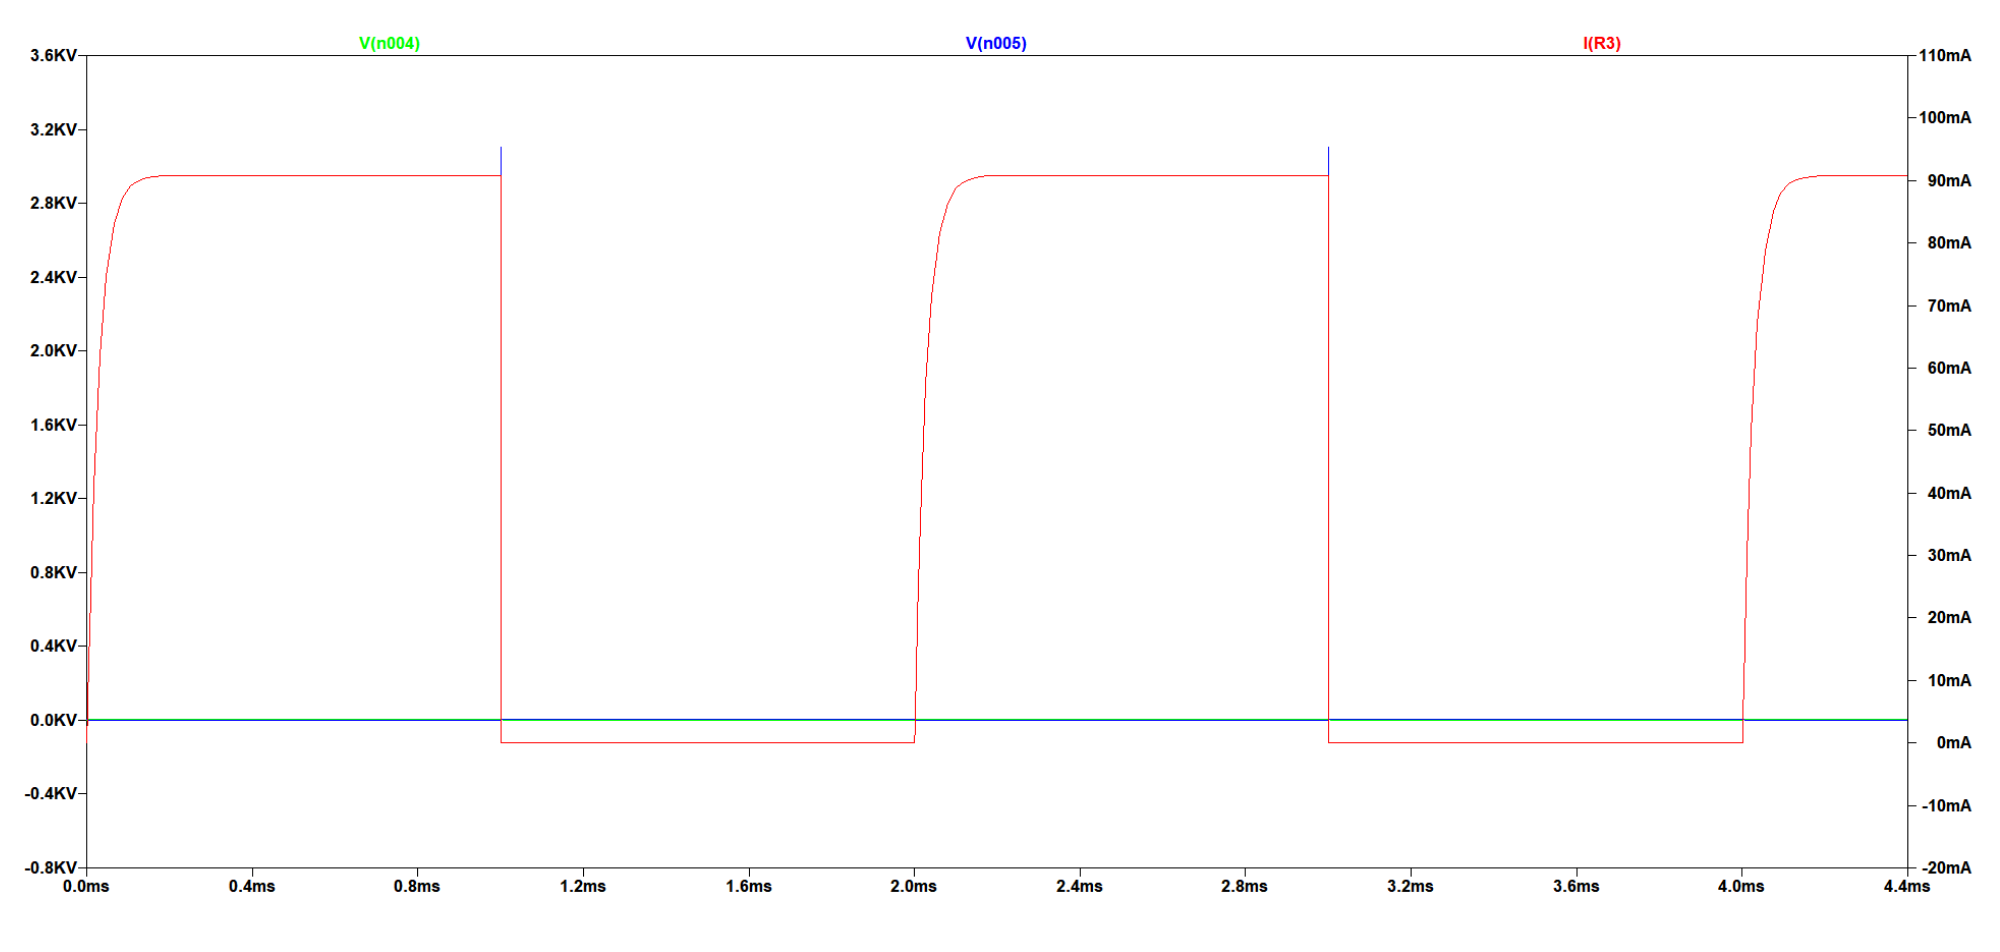
\includegraphics[
width=0.95\linewidth,
keepaspectratio
]{Metodologia/simulacao_sem_flyback.png}
\caption{Resposta transitória do circuito sem diodo de \textit{flyback}}
\label{fig:simulacao_sem_flyback}
\legend{Fonte: Elaboração própria (2026).}
\end{figure}

Nessa condição, a simulação apresentou transitórios de tensão mais pronunciados durante o desligamento da carga.

A comparação entre os dois cenários evidencia qualitativamente a função do diodo de \textit{flyback} no estágio de acionamento, justificando sua utilização em paralelo com o motor vibrotátil do protótipo.

Deve-se considerar, entretanto, que os valores absolutos obtidos dependem das simplificações adotadas no modelo elétrico e não devem ser interpretados como reprodução exata do comportamento físico do motor Vibracall 1027.




\subsection{Comportamento do Controle PWM}
\markright{Resultados e Discussão}
\label{sec:resultado_pwm_simulacao}

As simulações realizadas com diferentes valores de \textit{duty cycle} permitiram comparar o comportamento elétrico do modelo equivalente do atuador vibrotátil para diferentes níveis de comando PWM.

A Figura~\ref{fig:pwm20_resultado} apresenta a resposta obtida para um \textit{duty cycle} de 20\%.

\begin{figure}[!htbp]
    \centering
    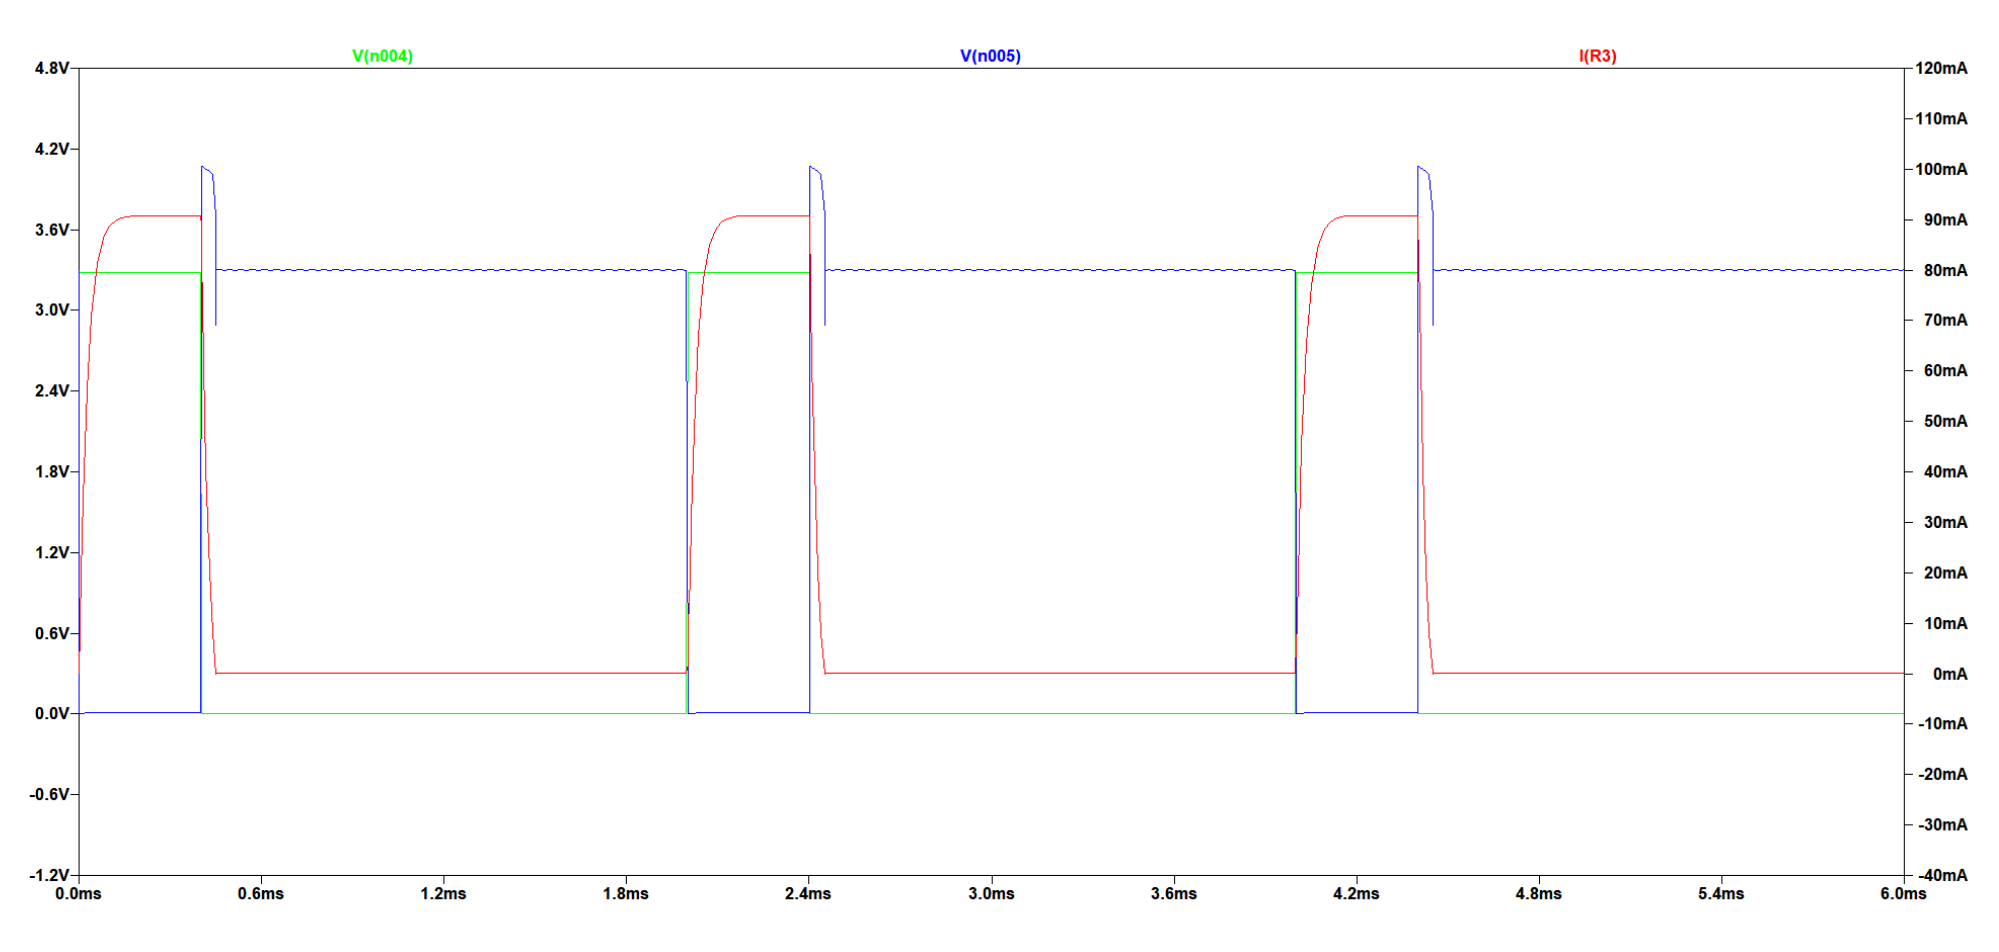
\includegraphics[
        width=0.95\linewidth,
        keepaspectratio
    ]{Metodologia/simulacao_pwm_20.png}
    \caption{Resposta simulada do circuito para \textit{duty cycle} de 20\%}
    \label{fig:pwm20_resultado}
\legend{Fonte: Elaboração própria (2026).}
\end{figure}

Nessa condição, o modelo apresentou o menor valor médio de corrente na carga entre os três cenários analisados.

A Figura~\ref{fig:pwm50_resultado} apresenta a resposta obtida para um \textit{duty cycle} de 50\%.

\begin{figure}[!htbp]
    \centering
    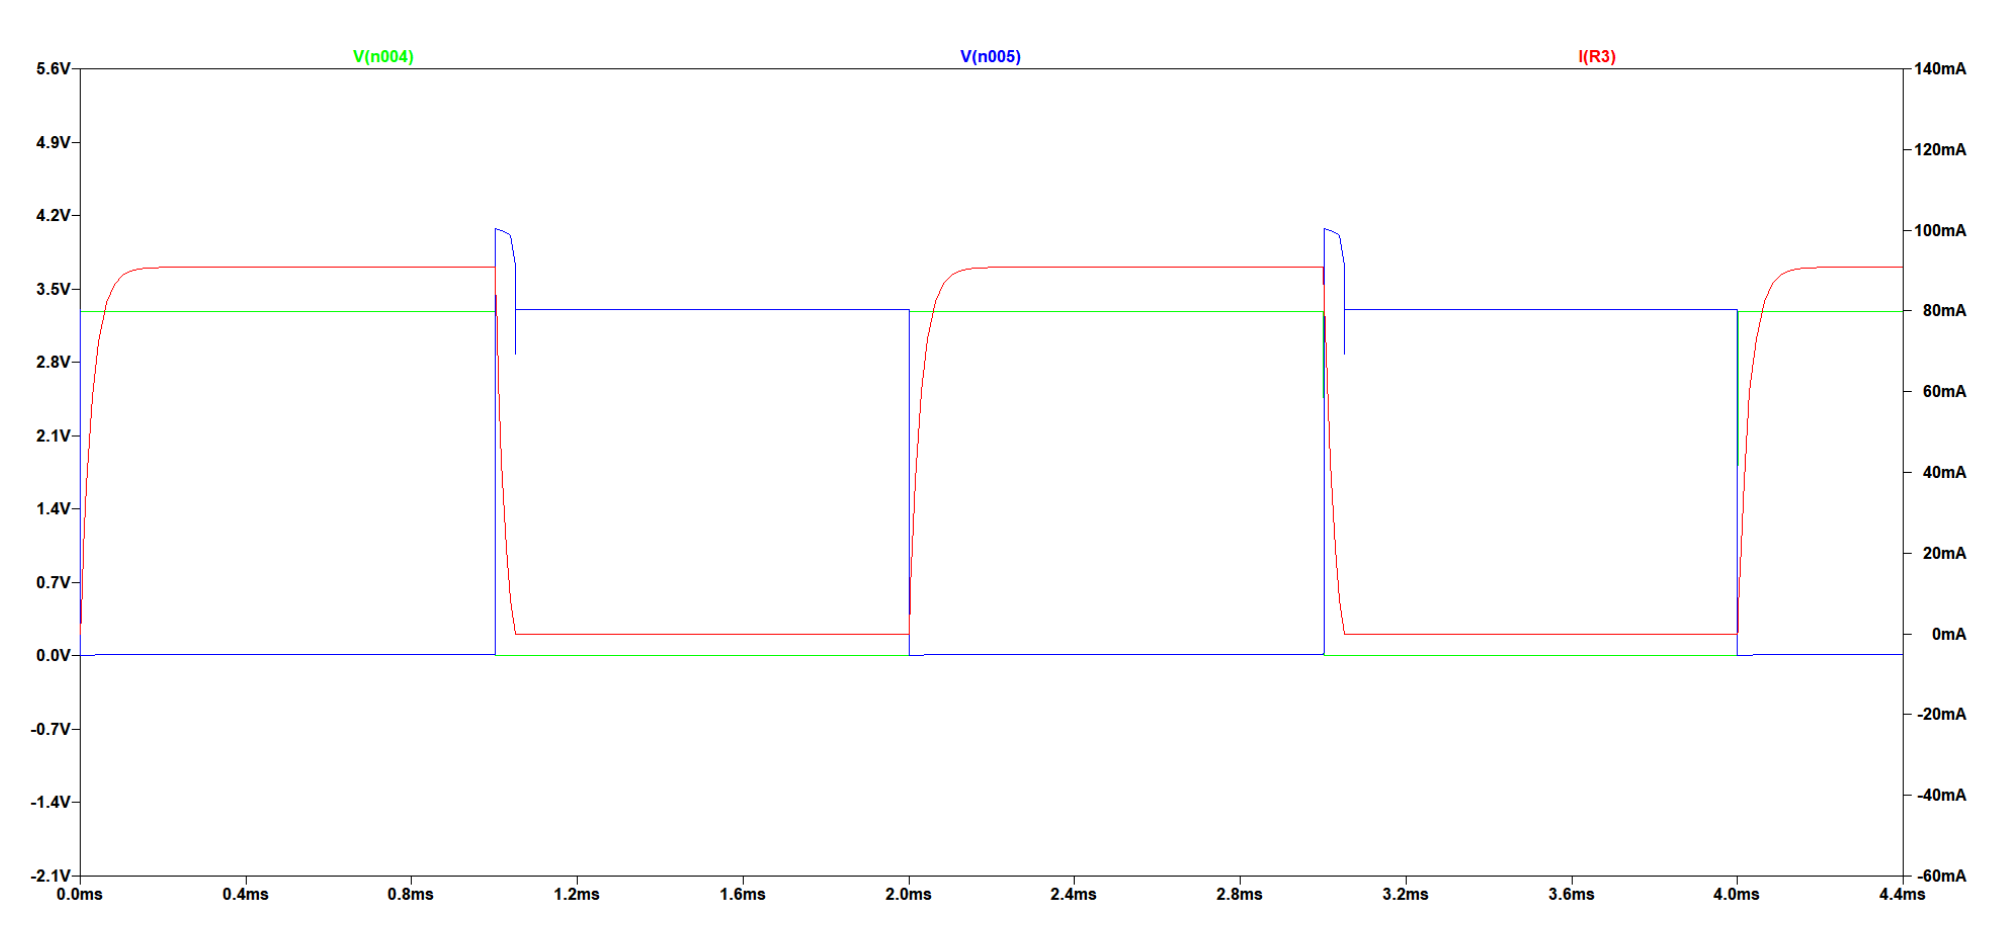
\includegraphics[
        width=0.95\linewidth,
        keepaspectratio
    ]{Metodologia/simulacao_pwm_50.png}
    \caption{Resposta simulada do circuito para \textit{duty cycle} de 50\%}
    \label{fig:pwm50_resultado}
\legend{Fonte: Elaboração própria (2026).}
\end{figure}

Para a condição intermediária, observou-se aumento do valor médio de corrente na carga em relação à condição de 20\%.

A Figura~\ref{fig:pwm80_resultado} apresenta a resposta obtida para um \textit{duty cycle} de 80\%.

\begin{figure}[!htbp]
    \centering
    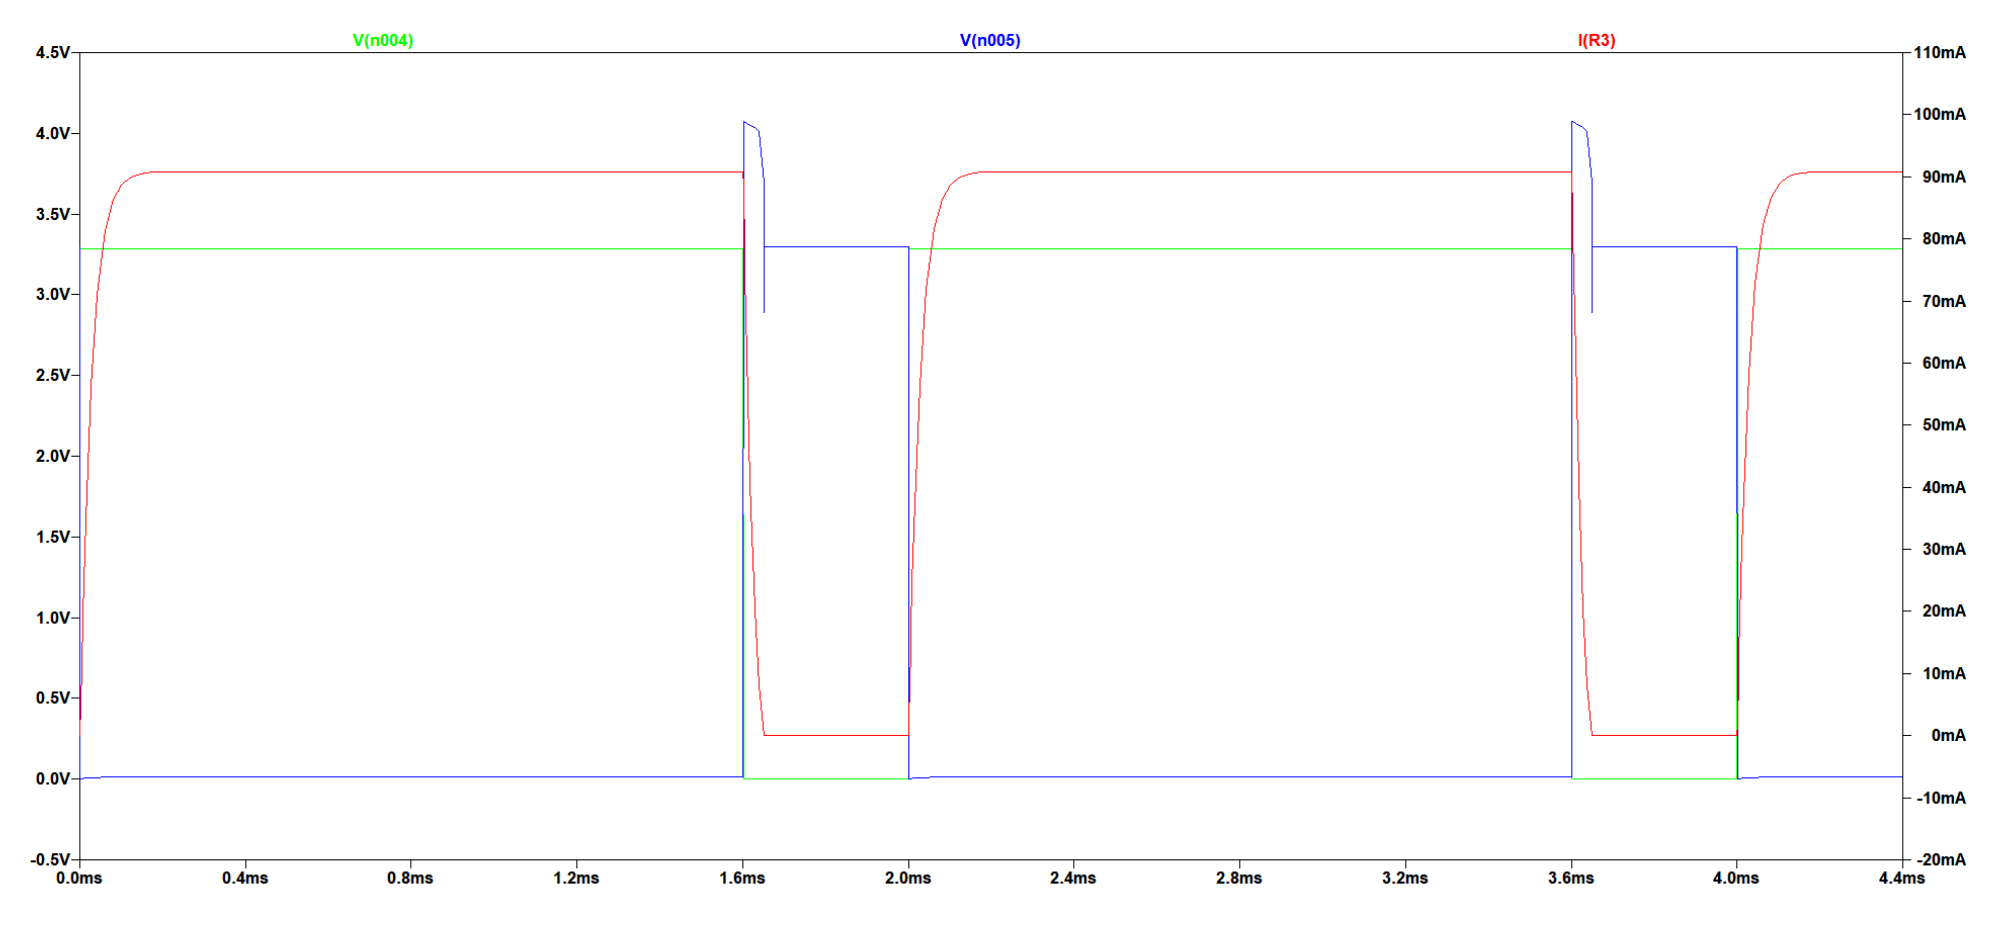
\includegraphics[
        width=0.95\linewidth,
        keepaspectratio
    ]{Metodologia/simulacao_pwm_80.png}
    \caption{Resposta simulada do circuito para \textit{duty cycle} de 80\%}
    \label{fig:pwm80_resultado}
\legend{Fonte: Elaboração própria (2026).}
\end{figure}

A condição de 80\% apresentou o maior valor médio de corrente entre os três cenários analisados.

A comparação entre as simulações de 20\%, 50\% e 80\% mostrou que o aumento do \textit{duty cycle} resulta em aumento da energia média fornecida à carga equivalente.

Esse comportamento é compatível com a estratégia adotada no protótipo, na qual o valor PWM é utilizado como variável de controle do canal vibrotátil.

Os resultados fornecem suporte elétrico para a utilização de diferentes valores PWM como níveis distintos de comando do motor Vibracall 1027.

Entretanto, as simulações não permitem estabelecer, por si só, uma relação quantitativa entre o valor PWM aplicado, a amplitude mecânica da vibração produzida pelo motor e a intensidade percebida pelo usuário.

Embora o mesmo valor PWM seja posteriormente utilizado como referência para o canal visual, as simulações apresentadas nesta seção representam exclusivamente o estágio eletrônico associado ao atuador vibrotátil e não caracterizam o comportamento luminoso do LED.


\section{Validação da Implementação Computacional}
\markright{Resultados e Discussão}
\label{sec:resultados_implementacao_computacional}


A implementação computacional foi avaliada inicialmente de forma independente do estágio físico de acionamento, conforme o procedimento descrito no Capítulo 4.

Essa etapa permitiu verificar a aquisição dos eventos MIDI, a extração do parâmetro \textit{velocity}, o cálculo dos valores PWM e a geração dos comandos antes da integração completa com o ESP32 e com as modalidades físicas de feedback.

Também foi verificado o funcionamento da interface gráfica desenvolvida para acompanhamento da interação, permitindo observar durante os ensaios o pad acionado, o valor de \textit{velocity} e o valor PWM calculado.

\subsection{Aquisição e Processamento dos Eventos MIDI}
\markright{Resultados e Discussão}
\label{sec:resultado_aquisicao_midi}

Durante os ensaios, o software desenvolvido em Python identificou os eventos MIDI provenientes do controlador Akai MPD218 e registrou os parâmetros associados às interações realizadas com os pads.

Os registros permitiram acompanhar informações como o tipo de evento, o número da nota MIDI e o valor de \textit{velocity}.

Para os eventos válidos de acionamento, o parâmetro \textit{velocity} foi extraído e encaminhado à etapa de cálculo do comando PWM. O número da nota MIDI foi utilizado para identificar o pad correspondente na interface gráfica.

A aquisição dos eventos e a geração dos comandos correspondentes foram registradas pelo próprio software, permitindo acompanhar a propagação das informações entre a entrada MIDI, a lógica de controle e a interface visual.

Os resultados confirmaram o funcionamento da etapa computacional responsável pela transformação dos eventos provenientes da interface musical em variáveis utilizadas posteriormente no controle das modalidades de feedback vibrotátil e visual.

\subsection{Mapeamento entre \textit{Velocity} e PWM}
\markright{Resultados e Discussão}
\label{sec:resultado_mapeamento_velocity_pwm}

A validação do mapeamento utilizou os valores de \textit{velocity} registrados durante a interação com o MPD218 e os comandos PWM calculados pelo software. A Figura~\ref{fig:curva_velocity_pwm} reúne os dados obtidos e a curva de escalonamento correspondente.

\begin{figure}[!htbp]
\centering
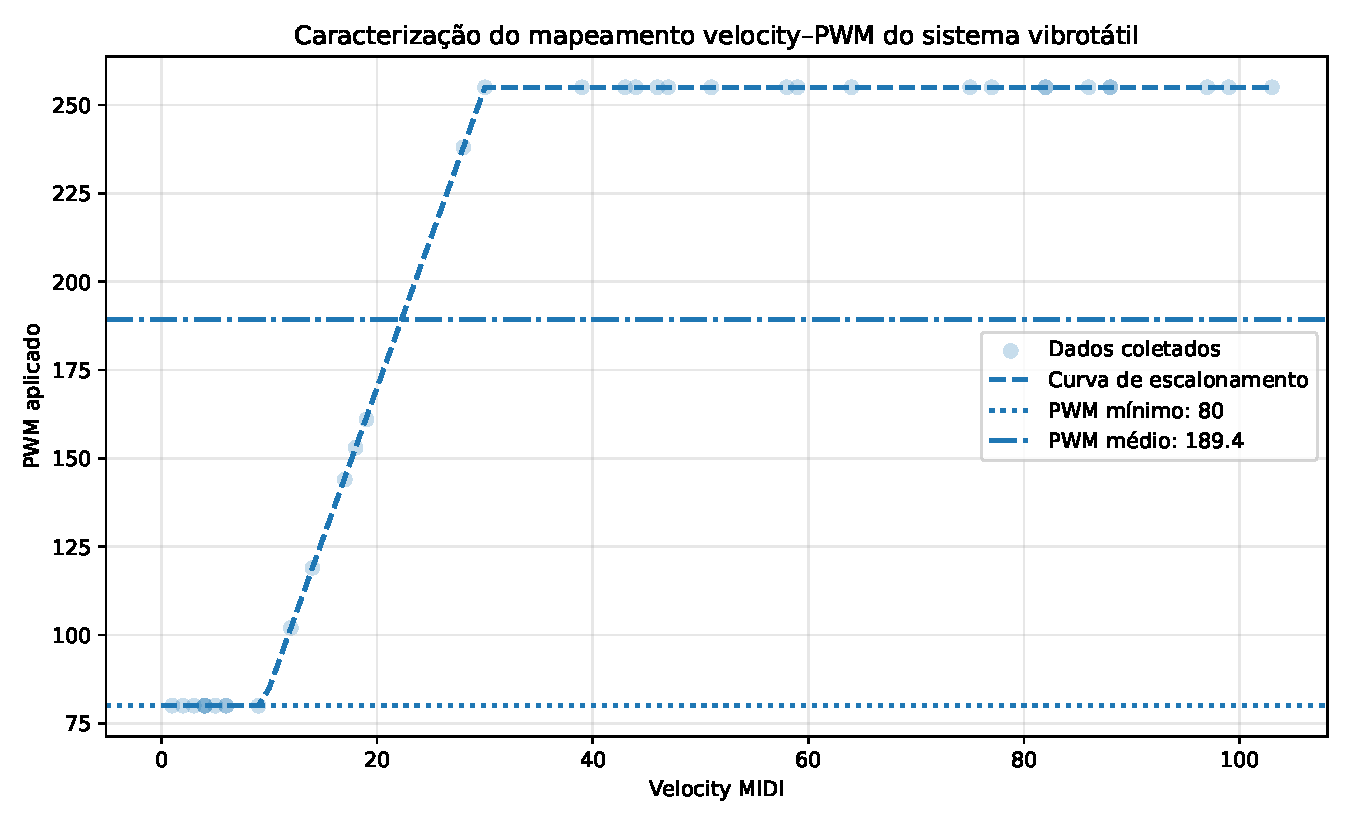
\includegraphics[width=0.85\linewidth,keepaspectratio]{Metodologia/grafico_velocity_pwm_final.pdf}
\caption{Relação experimental entre \textit{velocity} MIDI e valor PWM calculado}
\label{fig:curva_velocity_pwm}
\legend{Fonte: Elaboração própria (2026).}
\end{figure}

Os registros confirmaram o comportamento previsto pelo algoritmo: os comandos permaneceram entre 80 e 255, com limite inferior para acionamentos válidos, crescimento proporcional na região intermediária e saturação no valor máximo. A média dos valores PWM registrada no conjunto representado foi de 189,4. Essa relação é digital e não permite inferir uma proporcionalidade entre o comando e a intensidade mecânica ou luminosa percebida.

Nos ensaios posteriores com estímulo mecânico controlado, o MPD218 produziu frequentemente valores de \textit{velocity} superiores a 30, referência utilizada no programa principal. Para evitar a saturação precoce na caracterização experimental da Seção~\ref{sec:resultado_queda_controlada}, foi empregado um programa distinto que distribui a faixa MIDI de 1 a 127 entre PWM 80 e 255. As duas estratégias estão documentadas nos arquivos complementares do projeto.

\section{Resultados da Comunicação UDP}
\markright{Resultados e Discussão}
\label{sec:resultados_udp}


O procedimento de avaliação da comunicação UDP descrito na Seção~\ref{sec:teste_estabilidade_udp} foi utilizado para verificar o comportamento da transmissão sucessiva de comandos entre o software desenvolvido em Python e o microcontrolador ESP32.

O ensaio foi realizado com o envio de 100 pacotes numerados sequencialmente, com intervalo aproximado de 50~ms entre transmissões consecutivas, após a mensagem preliminar de inicialização definida na metodologia.

A análise considerou tanto a correspondência entre os identificadores transmitidos e recebidos quanto o comportamento temporal observado durante a sequência experimental.

\subsection{Recepção dos Pacotes}
\markright{Resultados e Discussão}
\label{sec:resultado_recepcao_udp}

A comparação entre os registros de transmissão e recepção mostrou que os 100 pacotes considerados no ensaio foram registrados pelo ESP32.

A figura a seguir apresenta os registros obtidos nos terminais utilizados durante o experimento.

\begin{figure}[!htbp]
\centering
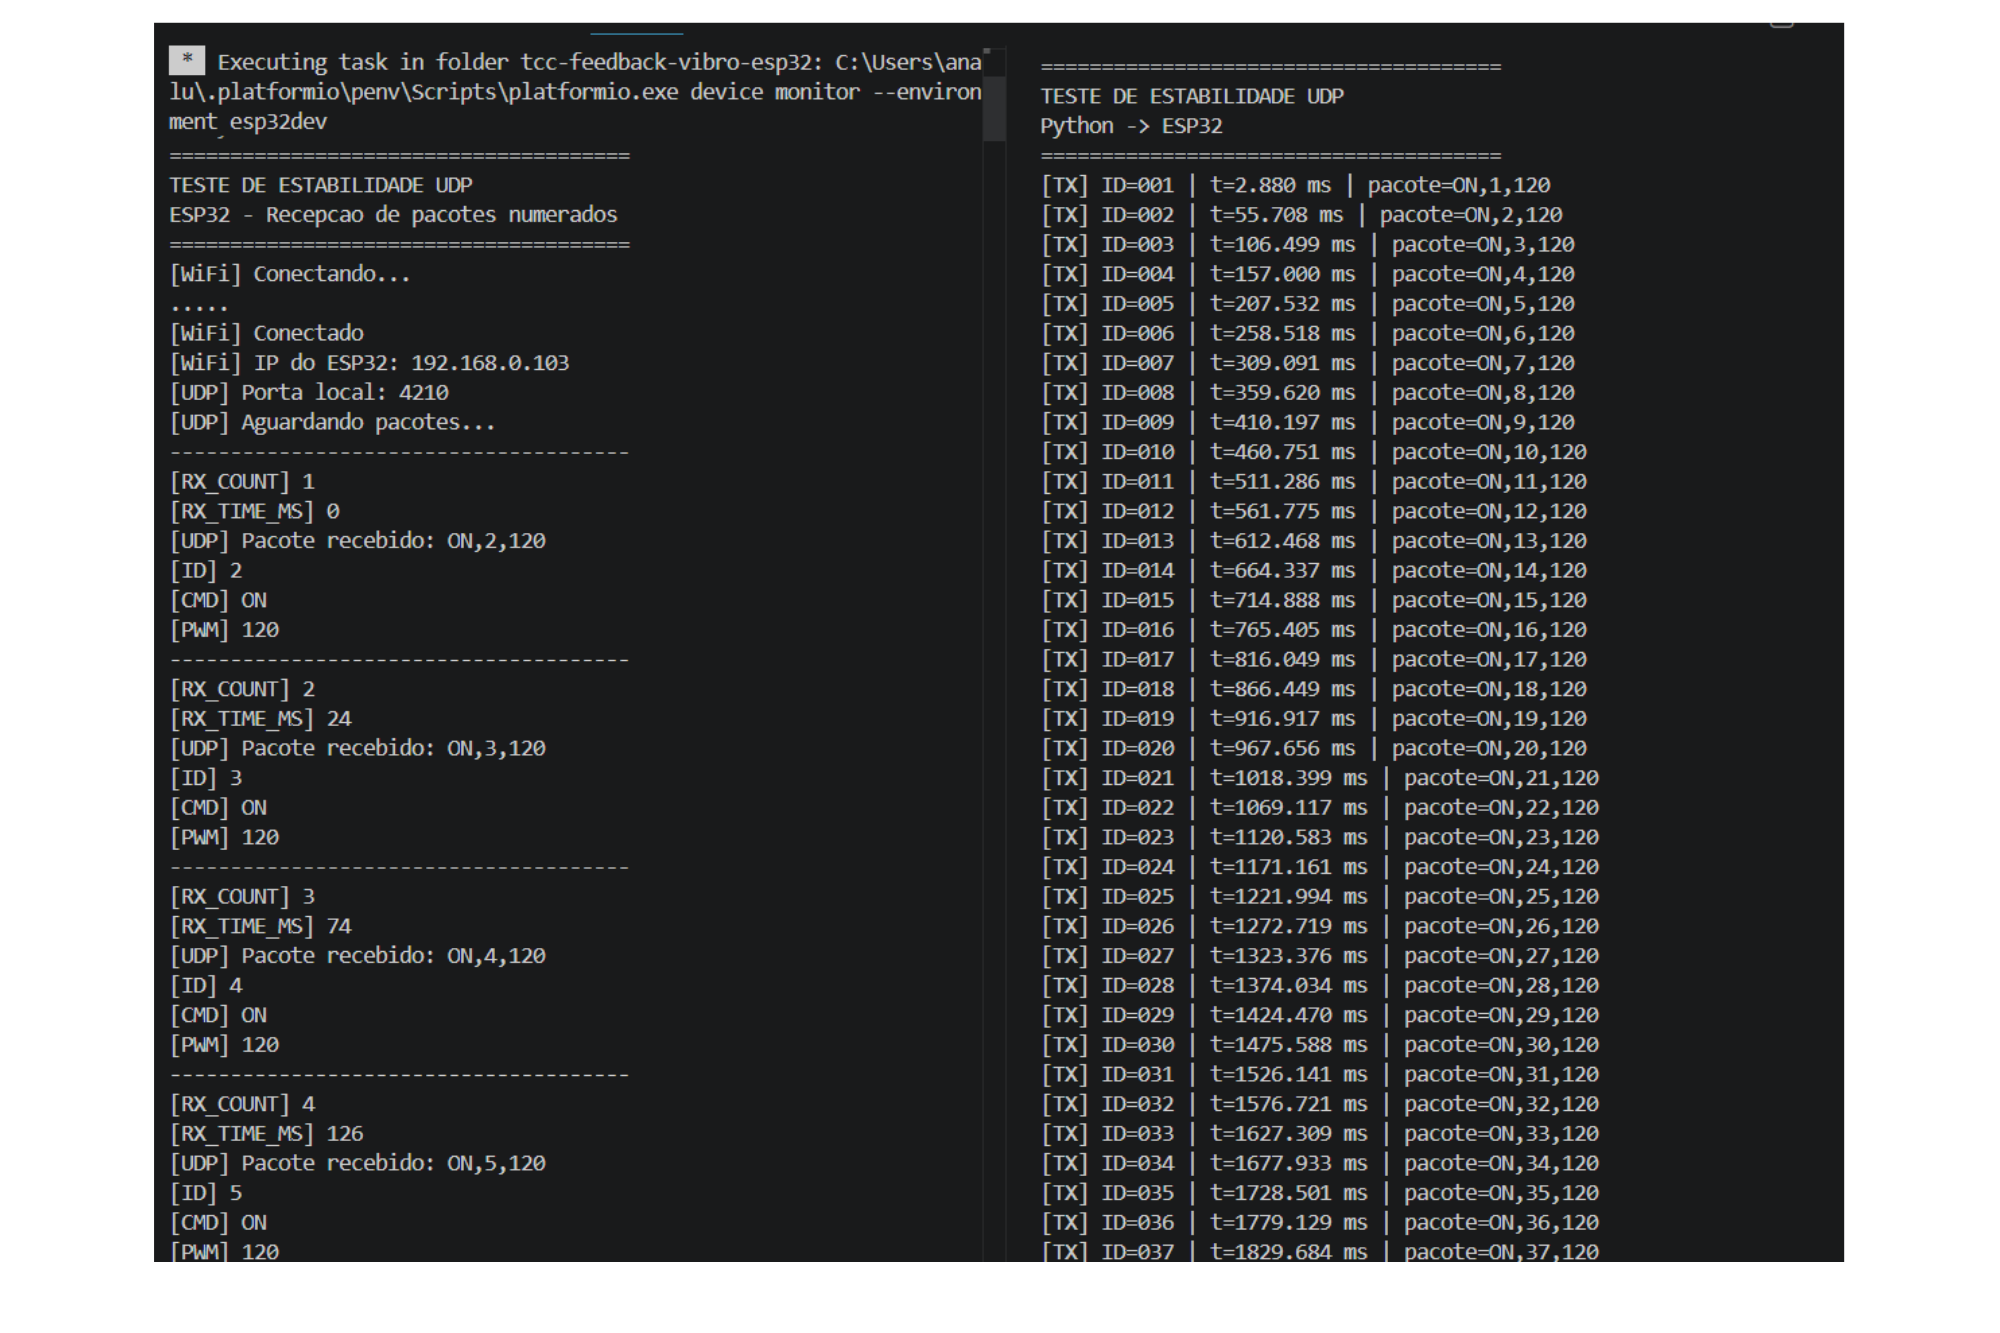
\includegraphics[
width=0.98\linewidth,
keepaspectratio
]{Metodologia/teste_estabilidade_terminal.png}
\caption{Registros do teste de transmissão de pacotes UDP entre Python e ESP32}
\label{fig:teste_estabilidade_udp_terminal}
\legend{Fonte: Elaboração própria (2026).}
\end{figure}

No terminal do software desenvolvido em Python foram registrados os identificadores dos pacotes transmitidos, enquanto o monitor serial do ESP32 permitiu acompanhar os identificadores efetivamente recebidos pelo microcontrolador.

Para a sequência analisada, foi observada correspondência entre os identificadores enviados e recebidos.

Os 100 datagramas considerados no ensaio foram registrados pelo ESP32, não sendo observada perda de pacotes na sequência utilizada para essa avaliação.

Esse resultado atende ao critério de validação estabelecido para a comunicação nas condições experimentais adotadas.

Entretanto, esse resultado deve ser interpretado dentro das condições específicas do ensaio. O protocolo UDP não incorpora mecanismos próprios de confirmação de entrega ou retransmissão e a ausência de perdas nessa sequência não constitui garantia de entrega dos datagramas em outras condições de rede, períodos mais prolongados de operação ou ambientes com diferentes níveis de interferência.

\subsection{Comportamento Temporal da Comunicação}
\markright{Resultados e Discussão}
\label{sec:resultado_temporal_udp}

Além da correspondência entre os pacotes transmitidos e recebidos, foram analisados os registros temporais produzidos durante o ensaio.

A figura a seguir apresenta o comportamento temporal da sequência de pacotes registrada pelo ESP32.

\begin{figure}[!htbp]
\centering
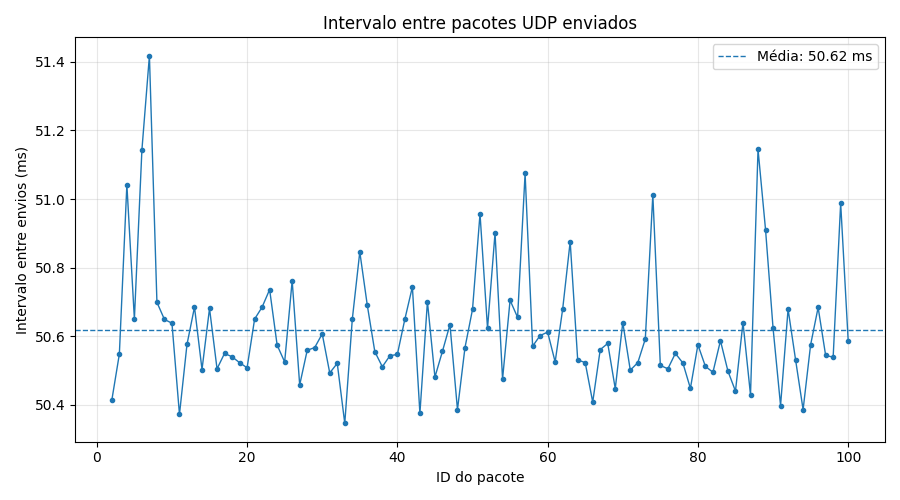
\includegraphics[
width=0.90\linewidth,
keepaspectratio
]{Metodologia/grafico_estabilidade_udp.png}
\caption{Comportamento temporal da recepção dos pacotes UDP durante o ensaio}
\label{fig:grafico_estabilidade_udp}
\legend{Fonte: Elaboração própria (2026).}
\end{figure}

Os registros apresentaram progressão temporal compatível com a transmissão sucessiva configurada no software, cujo intervalo nominal entre pacotes foi definido em aproximadamente 50~ms.

Foram observadas pequenas variações entre os intervalos de recepção ao longo da sequência.

Esse comportamento é compatível com a natureza não determinística da cadeia de comunicação utilizada, que envolve a execução do software no computador, a transmissão pela rede Wi-Fi, o processamento realizado pelo ESP32 e o próprio registro das informações pelo monitor serial.

Nas condições avaliadas, essas variações não impediram a recepção da sequência completa de pacotes considerada no ensaio.

O resultado permite caracterizar o funcionamento da comunicação UDP durante o procedimento realizado, mas não corresponde a uma medição da latência fim a fim do sistema.

Os instantes utilizados no computador e no ESP32 foram obtidos em plataformas distintas e sem uma referência temporal comum de alta precisão. Dessa forma, esses registros não foram utilizados para determinar quantitativamente o tempo transcorrido entre o acionamento de um pad MIDI e o início da resposta física do motor ou do LED.

Consequentemente, os resultados desta etapa sustentam a estabilidade funcional da transmissão nas condições experimentais adotadas, sem permitir classificar formalmente a arquitetura como um sistema de tempo real.

\section{Validação Física do Sistema Multissensorial}

A validação física do sistema foi realizada de forma incremental, conforme os procedimentos descritos no Capítulo 4.

A sequência de ensaios compreendeu inicialmente a verificação do estágio eletrônico utilizando uma carga auxiliar de teste, seguida pela validação do canal vibrotátil, integração da alimentação embarcada, incorporação do feedback visual e, por fim, operação simultânea das modalidades tátil e visual com a unidade vestível alimentada pelas baterias.

Essa abordagem permitiu verificar individualmente os principais módulos físicos antes da operação integrada da arquitetura.


\subsection{Validação do Estágio de Chaveamento}
\markright{Resultados e Discussão}

Na etapa inicial de validação física, um LED foi utilizado como carga auxiliar de teste no estágio de chaveamento baseado no transistor MOSFET IRLZ44N.

A aplicação dos comandos de controle permitiu verificar o caminho formado pelo GPIO do ESP32, resistor de gate, transistor MOSFET e carga conectada à saída.

A resposta observada confirmou a capacidade do ESP32 de comandar o estágio eletrônico antes da conexão do motor vibrotátil.

Esse procedimento reduziu o risco associado à integração inicial com a carga indutiva e permitiu prosseguir para a utilização do atuador Vibracall 1027.

O LED empregado nessa etapa teve função exclusivamente auxiliar de depuração e não corresponde ao canal de feedback visual posteriormente incorporado à configuração final do protótipo.


\subsection{Validação do Canal Vibrotátil}
\markright{Resultados e Discussão}

Após a validação inicial do estágio de chaveamento, foi realizado o ensaio utilizando um motor Vibracall 1027 conectado ao circuito eletrônico.

Durante a primeira etapa de depuração, foram realizadas medições de tensão e testes de continuidade entre o GPIO 18 do ESP32, o resistor de gate e o terminal de controle do MOSFET.

Foi identificada uma falha de contato no caminho entre a saída do microcontrolador e o estágio de gate, impedindo que o nível lógico produzido pelo ESP32 chegasse adequadamente ao transistor.

Após a correção da conexão, foi verificada a presença de aproximadamente 3,3~V no estágio de controle durante a condição de acionamento.

Em seguida, comandos UDP foram enviados diretamente ao ESP32 para verificar o acionamento e o desligamento do motor.

O Vibracall 1027 passou a responder corretamente aos comandos recebidos, confirmando o funcionamento da cadeia formada pela comunicação UDP, geração do sinal PWM, estágio de chaveamento e atuador vibrotátil.

Posteriormente, o controlador Akai MPD218 foi utilizado como fonte dos eventos de entrada. O software desenvolvido em Python processou os valores de \textit{velocity}, calculou os respectivos comandos PWM e realizou sua transmissão ao ESP32.

Durante esse ensaio, o motor apresentou acionamento durante os eventos válidos e desligamento após o término da interação, confirmando o funcionamento do canal vibrotátil utilizando a cadeia completa de controle prevista na arquitetura.



\subsection{Resposta do MPD218 ao Ensaio com Corpo de Massa Conhecida}
\markright{Resultados e Discussão}
\label{sec:resultado_queda_controlada}

O ensaio com o corpo de 39~g permitiu avaliar a resposta do controlador sob condições de impacto progressivamente maiores. Foram realizadas dez repetições em cada uma das seis alturas definidas na metodologia, totalizando 60 quedas independentes. Em cada repetição foi considerado apenas o primeiro evento MIDI válido após o armamento do programa; os eventos subsequentes ocorridos dentro da janela temporal de filtragem foram registrados separadamente como repiques. O procedimento e o corpo utilizado são apresentados na Figura~\ref{fig:ensaio_queda_massa}, enquanto o ensaio exploratório que antecedeu a definição da metodologia é registrado na Figura~\ref{fig:ensaio_estatico_exploratorio}.

Nos ensaios exploratórios anteriores à coleta definitiva, foi registrada uma condição próxima de 579~g para a ocorrência de acionamento no carregamento estático do \textit{pad}, documentado na Figura~\ref{fig:ensaio_estatico_exploratorio}. Esse valor foi mantido como observação preliminar e não integrou a análise quantitativa principal. Alturas de queda superiores a 5~cm produziram ocorrência frequente do valor máximo de \textit{velocity}, igual a 127, além de impactos progressivamente mais severos sobre o controlador. Durante os ensaios preliminares observou-se que, após o primeiro contato com o \textit{pad}, o corpo podia retornar à superfície e produzir um ou mais eventos MIDI adicionais, motivando a filtragem de repiques descrita na Seção~\ref{sec:filtragem_repiques}.

A Tabela~\ref{tab:queda_velocity_pwm} resume os resultados obtidos. Além da média, são apresentados o desvio-padrão e a mediana da \textit{velocity}, de modo a evidenciar a dispersão observada principalmente nas menores alturas. Os valores de PWM correspondem ao mapeamento específico utilizado neste ensaio, com a faixa MIDI de 1 a 127 distribuída entre PWM 80 e 255.

\begin{table}[!htbp]
\centering
\caption{Resultados do ensaio com corpo de 39~g para diferentes alturas de queda}
\label{tab:queda_velocity_pwm}
\resizebox{\textwidth}{!}{
\begin{tabular}{c c c c c c c}
\hline
Altura (cm) & $E_p$ (J) & \textit{Velocity} média $\pm$ DP & Mediana & PWM médio $\pm$ DP & Repiques & $v=127$ \\
\hline
0,5 & 0,001912 & 38,6 $\pm$ 19,91 & 41,0 & 132,2 $\pm$ 27,61 & 0 & 0 \\
1,0 & 0,003825 & 76,9 $\pm$ 26,49 & 87,0 & 185,5 $\pm$ 36,70 & 4 & 0 \\
2,0 & 0,007649 & 99,4 $\pm$ 9,29 & 102,0 & 216,6 $\pm$ 12,93 & 8 & 0 \\
3,0 & 0,011474 & 108,5 $\pm$ 5,56 & 111,0 & 229,3 $\pm$ 7,90 & 7 & 0 \\
4,0 & 0,015298 & 116,3 $\pm$ 7,72 & 118,5 & 240,0 $\pm$ 10,61 & 4 & 0 \\
5,0 & 0,019123 & 124,5 $\pm$ 2,01 & 124,5 & 251,4 $\pm$ 2,88 & 3 & 3 \\
\hline
\end{tabular}
}
\legend{Fonte: Elaboração própria (2026).}
\end{table}

Observa-se crescimento sucessivo da média de \textit{velocity} ao longo de todas as condições avaliadas. O valor médio passou de 38,6 na altura de 0,5~cm para 124,5 em 5~cm. Como o PWM foi calculado a partir da \textit{velocity}, a mesma tendência foi preservada na variável de controle, cuja média aumentou de 132,2 para 251,4.

A dispersão foi mais elevada nas duas menores alturas. Para 0,5~cm e 1~cm, os desvios-padrão de \textit{velocity} foram, respectivamente, 19,91 e 26,49. A partir de 2~cm, a variabilidade diminuiu de forma acentuada, com desvios entre 2,01 e 9,29. As observações válidas das menores alturas foram mantidas na análise, inclusive quando apresentaram valores reduzidos, pois correspondiam ao primeiro impacto registrado após o armamento da repetição e não atendiam ao critério definido para classificação como repique.

Na condição de 5~cm, três das dez repetições atingiram o limite superior do protocolo MIDI, com \textit{velocity} igual a 127. Esse comportamento indica o início de uma região de saturação do próprio controlador para as condições adotadas. A escolha de alturas mais elevadas tenderia a reduzir a capacidade do ensaio de distinguir novos aumentos na intensidade do impacto.

A associação entre altura de queda e \textit{velocity} foi avaliada a partir das 60 observações individuais. O coeficiente de Spearman foi $\rho=0{,}944$ ($p<0{,}001$), indicando associação monotônica forte entre o aumento da altura e a resposta fornecida pelo MPD218. Como medida complementar, o coeficiente de Pearson foi $r=0{,}818$ ($p<0{,}001$). A diferença entre os dois coeficientes é compatível com a forma não estritamente linear da resposta e com a aproximação do limite superior de \textit{velocity} nas maiores alturas.

Esses resultados não representam uma medição direta da força de impacto. Para massa constante, o aumento da altura elevou a energia potencial disponível antes da queda e a velocidade teórica imediatamente anterior ao contato. O ensaio mostra que condições mecânicas de entrada progressivamente maiores produziram, em média, valores também maiores de \textit{velocity}, que foram convertidos em níveis crescentes de PWM pelo programa de teste.

A Figura~\ref{fig:altura_velocity_ensaio} apresenta a evolução da média de \textit{velocity} em função da altura de queda. As barras verticais correspondem a um desvio-padrão em torno da média de cada condição.

\begin{figure}[!htbp]
\centering
\begin{tikzpicture}
\begin{axis}[
    width=0.88\textwidth,
    height=0.52\textwidth,
    xlabel={Altura de queda (cm)},
    ylabel={\textit{Velocity} MIDI},
    xmin=0.25,
    xmax=5.25,
    ymin=0,
    ymax=135,
    xtick={0.5,1,2,3,4,5},
    xticklabels={{0,5},1,2,3,4,5},
    ytick={0,20,40,60,80,100,120},
    grid=major,
    major grid style={line width=.2pt,draw=gray!40},
    axis line style={black},
    tick style={black},
    tick label style={font=\small},
    label style={font=\small},
    legend style={font=\small,draw=none,at={(0.03,0.97)},anchor=north west},
]
\addplot+[
    color=black,
    mark=*,
    thick,
    error bars/.cd,
    y dir=both,
    y explicit
] coordinates {
    (0.5,38.6) +- (0,19.91)
    (1,76.9)   +- (0,26.49)
    (2,99.4)   +- (0,9.29)
    (3,108.5)  +- (0,5.56)
    (4,116.3)  +- (0,7.72)
    (5,124.5)  +- (0,2.01)
};
\end{axis}
\end{tikzpicture}
\caption{Valor médio de \textit{velocity} em função da altura de queda do corpo de 39~g. As barras representam $\pm 1$ desvio-padrão.}
\label{fig:altura_velocity_ensaio}
\legend{Fonte: Elaboração própria (2026).}
\end{figure}




\subsection{Caracterização Acústica do Atuador em Função do PWM}
\markright{Resultados e Discussão}
\label{sec:resultado_acustico_pwm}

A caracterização acústica foi utilizada como uma segunda forma de observar o comportamento do motor diante de diferentes níveis de comando. Para cada valor de PWM foram analisadas três repetições, obtidas a partir da sequência automatizada de acionamento descrita na Seção~\ref{sec:ensaio_acustico_pwm}. A montagem utilizada para a captação é apresentada na Figura~\ref{fig:ensaio_microfone_condensador}.

A Tabela~\ref{tab:frequencia_pwm} apresenta as frequências acústicas identificadas em cada repetição, além da média, do desvio-padrão e do coeficiente de variação de cada condição.

\begin{table}[!htbp]
\centering
\caption{Frequência acústica associada ao funcionamento do motor para diferentes valores PWM}
\label{tab:frequencia_pwm}
\resizebox{\textwidth}{!}{
\begin{tabular}{c c c c c c c}
\hline
PWM & Rep. 1 (Hz) & Rep. 2 (Hz) & Rep. 3 (Hz) & Média (Hz) & DP (Hz) & CV (\%) \\
\hline
80  & 91,5  & 92,9  & 90,2  & 91,5  & 1,35  & 1,5 \\
115 & 106,3 & 127,9 & 126,5 & 120,2 & 12,09 & 10,1 \\
150 & 145,3 & 154,8 & 165,5 & 155,2 & 10,11 & 6,5 \\
185 & 173,6 & 191,1 & 196,5 & 187,1 & 11,97 & 6,4 \\
220 & 203,2 & 212,6 & 216,7 & 210,8 & 6,92  & 3,3 \\
255 & 224,8 & 227,4 & 231,5 & 227,9 & 3,38  & 1,5 \\
\hline
\end{tabular}
}
\legend{Fonte: Elaboração própria (2026).}
\end{table}

A frequência média aumentou em todas as etapas do ensaio, passando de aproximadamente 91,5~Hz para PWM 80 a 227,9~Hz para PWM 255. Considerando as 18 observações individuais, foi obtido coeficiente de Spearman $\rho=0{,}988$ ($p<0{,}001$) e coeficiente de Pearson $r=0{,}984$ ($p<0{,}001$). Os dois resultados indicam associação forte entre o nível de PWM aplicado e a frequência acústica identificada na gravação.

Como não havia um valor de referência nominal de frequência para cada nível de PWM nas condições específicas de montagem do protótipo, não foi calculado erro absoluto em relação a um valor verdadeiro. A repetibilidade foi caracterizada pelo desvio-padrão e pelo coeficiente de variação entre as três repetições. A maior dispersão relativa ocorreu em PWM 115, com coeficiente de variação de 10,1\%, enquanto as condições de PWM 80 e 255 apresentaram coeficiente de variação próximo de 1,5\%.

Também foi observada, em parte das condições intermediárias, tendência de aumento da frequência nas repetições posteriores. Como a sequência de PWM foi aplicada sempre em ordem crescente, o ensaio não permite separar completamente o efeito do comando de possíveis efeitos associados ao tempo de funcionamento, aquecimento do motor, alimentação ou acoplamento mecânico durante a gravação. Essa variação foi preservada nos resultados e incorporada às medidas de dispersão.

A medida acústica deve ser interpretada como um indicador indireto do comportamento do atuador. O ensaio não determina a amplitude mecânica da vibração nem substitui uma caracterização realizada com acelerômetro. Ainda assim, a progressão observada acrescenta evidência experimental de que níveis distintos de PWM produzem estados dinâmicos distintos no motor.

Em conjunto com o ensaio de queda controlada, a caracterização estabelece experimentalmente a sequência entre uma entrada mecânica de maior intensidade, o aumento da \textit{velocity} MIDI, o aumento do comando PWM e a alteração da frequência acústica associada ao funcionamento do atuador.

A Figura~\ref{fig:pwm_frequencia_acustica} sintetiza a relação entre o comando PWM e a frequência acústica média identificada no atuador. As barras verticais representam um desvio-padrão calculado a partir das três repetições de cada condição.

\begin{figure}[!htbp]
\centering
\begin{tikzpicture}
\begin{axis}[
    width=0.88\textwidth,
    height=0.52\textwidth,
    xlabel={Valor PWM},
    ylabel={Frequência acústica dominante (Hz)},
    xmin=70,
    xmax=265,
    ymin=70,
    ymax=245,
    xtick={80,115,150,185,220,255},
    ytick={80,100,120,140,160,180,200,220,240},
    grid=major,
    major grid style={line width=.2pt,draw=gray!40},
    axis line style={black},
    tick style={black},
    tick label style={font=\small},
    label style={font=\small},
]
\addplot+[
    color=black,
    mark=square*,
    thick,
    error bars/.cd,
    y dir=both,
    y explicit
] coordinates {
    (80,91.5)   +- (0,1.35)
    (115,120.2) +- (0,12.09)
    (150,155.2) +- (0,10.11)
    (185,187.1) +- (0,11.97)
    (220,210.8) +- (0,6.92)
    (255,227.9) +- (0,3.38)
};
\end{axis}
\end{tikzpicture}
\caption{Frequência acústica média associada ao funcionamento do motor em função do valor PWM aplicado. As barras representam $\pm 1$ desvio-padrão.}
\label{fig:pwm_frequencia_acustica}
\legend{Fonte: Elaboração própria (2026).}
\end{figure}




\subsection{Validação da Alimentação Embarcada}
\markright{Resultados e Discussão}

Após a validação do protótipo utilizando alimentação de bancada, foi realizada a integração do sistema destinado à operação autônoma da unidade vestível.

O conjunto de alimentação foi constituído por duas células recarregáveis de íons de lítio em configuração 2S, módulo BMS e conversor DC--DC baseado no MP1584EN. O módulo empregado nessa etapa é mostrado na Figura~\ref{fig:modulo_mp1584en}.

Antes da conexão ao circuito, a tensão de saída do conversor foi ajustada para aproximadamente 3,3~V.

Com o ESP32 em funcionamento e conectado à rede Wi-Fi, foram realizadas medições diretamente no barramento de alimentação do microcontrolador.

Durante os ensaios, foram observados valores aproximadamente entre 3,26~V e 3,29~V, indicando manutenção da alimentação próxima ao valor definido para operação do circuito.

Também foram realizados testes auxiliares de conectividade entre o computador e o ESP32 utilizando o comando \texttt{ping}. Após os ajustes realizados no estágio de alimentação e nas conexões físicas da montagem, o microcontrolador permaneceu conectado à rede utilizando exclusivamente a alimentação proveniente das baterias.

Esse resultado confirmou funcionalmente a possibilidade de operação da unidade vestível sem utilização da alimentação USB do computador.

A avaliação realizada concentrou-se na estabilidade funcional da alimentação durante os ensaios. Não foram realizados testes destinados à determinação da autonomia total das baterias, consumo médio de corrente ou eficiência energética do conjunto.


\subsection{Validação do Feedback Visual}
\markright{Resultados e Discussão}

O LED respondeu aos estados de acionamento e desligamento durante os testes com comandos enviados diretamente ao ESP32.

A aplicação de diferentes valores PWM também produziu alterações correspondentes no nível de acionamento luminoso observado durante os ensaios.

Esses resultados confirmaram o funcionamento do canal visual como uma saída física independente do canal vibrotátil, embora ambas as modalidades utilizem o mesmo valor digital de controle.

A validação realizada foi de caráter funcional. Não foram efetuadas medições fotométricas nem avaliação perceptiva da intensidade luminosa produzida pelo LED.


\subsection{Operação Integrada da Arquitetura}
\markright{Resultados e Discussão}

Na etapa final da validação física, foi avaliada a operação integrada da cadeia formada pelo controlador Akai MPD218, software desenvolvido em Python, interface gráfica, comunicação UDP sobre rede Wi-Fi, microcontrolador ESP32, motor Vibracall 1027, LED de alto brilho e sistema de alimentação embarcado.

Durante a interação com os pads, os eventos MIDI foram capturados pelo software, que identificou o valor de \textit{velocity}, calculou o valor PWM correspondente e transmitiu o comando ao microcontrolador.

O ESP32 aplicou o mesmo valor de controle ao GPIO 18, associado ao canal vibrotátil, e ao GPIO 21, associado ao canal visual.

Durante os ensaios, o acionamento de um pad resultou simultaneamente na vibração do motor e no acionamento do LED. Ao término do evento MIDI, o comando de desligamento interrompeu simultaneamente as duas modalidades de saída.

A interface gráfica executada no computador também respondeu aos eventos, apresentando as informações associadas ao pad acionado, ao valor de \textit{velocity} e ao valor PWM calculado.

A unidade embarcada permaneceu alimentada pelo conjunto de baterias durante essa etapa, sem necessidade de alimentação do ESP32 por meio da interface USB.

A configuração vestível obtida ao final da integração é registrada na Figura~\ref{fig:prototipo_final_vestivel}. A fotografia documenta a disposição física alcançada após a passagem da montagem de bancada para a placa, o invólucro impresso e a pulseira de fixação.

Dessa forma, foi verificado experimentalmente o funcionamento integrado da cadeia:

\begin{center}
\text{MPD218}
$\rightarrow$
\text{Python}
$\rightarrow$
\text{UDP/Wi-Fi}
$\rightarrow$
\text{ESP32}
$\rightarrow$
\text{PWM}
$\rightarrow$
\text{feedback vibrotátil + feedback visual}
\end{center}

O resultado demonstra a viabilidade funcional da arquitetura desenvolvida para transformar informações provenientes da interação musical em respostas sensoriais tátil e visual utilizando uma unidade vestível com alimentação própria.

Essa conclusão permanece restrita ao funcionamento técnico do protótipo. Os ensaios realizados não permitem estabelecer, por si só, benefícios perceptivos, de acessibilidade ou terapêuticos sem avaliações posteriores com usuários.


\section{Discussão Integrada dos Resultados}

A avaliação conjunta dos subsistemas permite examinar a continuidade da informação entre o gesto no controlador MIDI e as respostas físicas da unidade vestível. Os ensaios de entrada, processamento, comunicação e atuação foram realizados separadamente antes da integração, o que possibilitou identificar falhas de montagem e distinguir a resposta de cada etapa.

Na entrada, o ensaio de queda mostrou associação monotônica entre a altura de liberação do corpo e a \textit{velocity} registrada. Essa caracterização também evidenciou uma limitação do mapeamento inicialmente empregado no programa principal: a referência superior de \textit{velocity} igual a 30 leva à saturação antecipada do comando PWM. O mapeamento completo utilizado na caracterização experimental preservou uma faixa maior de valores de controle, sem modificar retrospectivamente a configuração do programa original.

Na saída vibrotátil, as simulações sustentaram a escolha do diodo de \textit{flyback} para a proteção do estágio de chaveamento e mostraram a influência da razão cíclica sobre a carga elétrica equivalente. O ensaio acústico, por sua vez, identificou frequências distintas para diferentes comandos PWM. Essas observações são complementares, mas não estabelecem uma relação quantitativa entre \textit{velocity}, amplitude mecânica aplicada à pele e intensidade percebida; para isso, seriam necessárias medidas mecânicas diretas e avaliações com participantes.

A comunicação UDP permitiu a operação da cadeia nas condições do ensaio, com registro de todos os 100 datagramas avaliados. Esse resultado caracteriza a transmissão observada, mas não mede a latência entre o gesto MIDI e a resposta física, nem assegura o mesmo desempenho sob outras condições de rede. Assim, o funcionamento integrado não deve ser confundido com uma validação temporal de sistema em tempo real.

A alimentação embarcada permitiu operar o ESP32 sem conexão USB com o computador, e o LED acrescentou uma saída física independente do estágio do motor. Ambas as modalidades responderam ao comando comum, mas não foi estabelecida equivalência perceptiva entre brilho e vibração. A contribuição do protótipo está, portanto, na integração tecnicamente funcional desses módulos e na disponibilidade de uma plataforma reproduzível para avaliações futuras de acessibilidade musical.


\chapter{Conclusões}

\section{Considerações Finais}
\markright{Conclusões}
\label{sec:consideracoes_finais}

O objetivo deste trabalho foi desenvolver e validar tecnicamente uma interface musical digital multissensorial capaz de transformar informações do gesto no controlador Akai MPD218 em comandos para um motor vibrotátil e um LED incorporados a uma unidade vestível. Os resultados permitem responder afirmativamente à questão de viabilidade funcional proposta na Introdução, nas condições de implementação e ensaio descritas.

A cadeia composta por aquisição MIDI, processamento em Python, transmissão UDP sobre Wi-Fi, controle pelo ESP32 e acionamento das saídas foi verificada em etapas e em operação integrada. As simulações fundamentaram o circuito de proteção e o uso do PWM; os ensaios controlados caracterizaram relações mensuráveis entre altura de queda e \textit{velocity}, bem como entre PWM e frequência acústica associada ao motor. A alimentação por baterias permitiu a operação da unidade vestível sem conexão USB com o computador.

A caracterização experimental também indicou a necessidade de rever o mapeamento inicial que emprega referência superior de \textit{velocity} igual a 30, pois essa escolha antecipa a saturação dos comandos. O mapeamento de faixa completa utilizado nos ensaios constitui uma alternativa documentada, ainda não submetida a uma avaliação perceptiva.

A principal contribuição reside na arquitetura implementada e no conjunto de procedimentos técnicos disponibilizados para sua reprodução. O sistema representa ocorrência, duração e intensidade relativa de eventos MIDI, sem converter o conteúdo sonoro em uma reprodução tátil ou luminosa equivalente. A viabilidade demonstrada não permite concluir que a interface melhore a percepção musical de pessoas surdas ou com deficiência auditiva; essa avaliação exige participação da população-alvo em estudos específicos.

\section{Limitações do Protótipo}
\markright{Conclusões}
\label{sec:limitacoes_prototipo}

A principal limitação da caracterização vibrotátil é a ausência de medição inercial direta. O registro com microfone permitiu acompanhar a frequência acústica associada ao motor, mas não forneceu valores de aceleração, deslocamento ou amplitude de vibração. A relação entre PWM e intensidade mecânica transmitida à pele não foi quantificada.

A sequência do ensaio acústico foi executada sempre em ordem crescente de PWM. Variações entre repetições podem incluir efeitos de tempo de funcionamento, aquecimento, condição da alimentação ou acoplamento mecânico e acústico. A correlação observada sustenta a tendência entre comando e frequência registrada, mas não separa essas fontes de variabilidade.

O canal visual foi validado funcionalmente, sem medição fotométrica ou estudo de equivalência perceptiva com o canal tátil. O uso do mesmo valor PWM representa apenas uma estratégia comum de controle.

A comunicação UDP não foi caracterizada quanto à latência fim a fim, e os testes não abrangeram diferentes redes, distâncias ou condições de interferência. A alimentação embarcada também não foi avaliada em termos de autonomia, consumo médio, eficiência do conversor ou temperatura em operação prolongada.

A estrutura vestível foi utilizada como suporte experimental. Conforto prolongado, distribuição de massa, pressão de contato, estabilidade durante movimentos e posicionamento ótimo do motor não foram avaliados por protocolo específico.

A configuração física utilizou um único motor vibrotátil. Não foram avaliados arranjos com múltiplos atuadores, codificação espacial de eventos ou distribuição dos estímulos entre regiões do corpo.

Não foram realizados ensaios formais com pessoas surdas ou com deficiência auditiva. O trabalho não determina limiares de percepção, capacidade de discriminação entre níveis de estímulo, compreensão de padrões rítmicos, conforto de uso ou contribuição efetiva para a experiência musical. A validação é estritamente técnica.

\section{Propostas de Continuidade}
\markright{Conclusões}
\label{sec:propostas_continuidade}

A continuidade técnica mais direta consiste em medir a resposta do motor com acelerômetro fixado à estrutura vestível. Essa instrumentação permitiria relacionar o comando PWM à aceleração, à frequência mecânica e à amplitude do estímulo em condições controladas.

O mapeamento entre \textit{velocity} e PWM também deve ser revisto. Os ensaios mostraram que a referência superior igual a 30 comprime parte relevante da faixa dinâmica do MPD218. A distribuição da faixa completa de 1 a 127, ou uma função não linear ajustada experimentalmente, pode reduzir a saturação e preservar diferenças entre níveis de interação.

Novos ensaios do motor podem empregar ordem randomizada dos valores PWM, maior número de repetições e medição simultânea de tensão, corrente e aceleração. No canal visual, medições fotométricas permitiriam caracterizar a relação entre PWM e brilho e, posteriormente, definir mapeamentos independentes para as modalidades tátil e visual.

A latência fim a fim também pode ser medida com uma referência temporal comum entre o acionamento do pad e as saídas físicas. Esse procedimento permitiria separar os atrasos de aquisição MIDI, processamento em Python, transmissão Wi-Fi, recepção pelo ESP32 e atuação.

Na alimentação, ensaios de autonomia, consumo e temperatura podem orientar a escolha das células e a evolução para uma placa dedicada e uma estrutura mais compacta. A integração mecânica também pode ser refinada para reduzir volume e melhorar o contato do atuador com a pele.

A etapa decisiva para o objetivo de acessibilidade é a avaliação participativa com pessoas surdas ou com deficiência auditiva. Estudos futuros podem investigar discriminação de intensidade, pulsação, ritmo e padrões temporais, além de conforto, preferência e facilidade de aprendizagem. A participação da população-alvo e de profissionais ligados à comunidade surda pode orientar decisões de mapeamento que não podem ser estabelecidas apenas por ensaios técnicos.


% Elementos pós-textuais
\postextual
\begin{SingleSpace}
\setlength{\bibitemsep}{\baselineskip}
\printbibliography[heading=bibintoc,title={Referências}]
\end{SingleSpace}

% Apêndice com documentação complementar de reprodução
% Apêndice A: arquivos complementares para reprodução técnica do protótipo.
% O ambiente apendicesenv gera automaticamente "APÊNDICE A" no título e no sumário.
\begin{apendicesenv}
\chapter{Arquivos complementares para reprodução do protótipo}
\label{ap:arquivos_complementares}

Com a finalidade de disponibilizar os recursos utilizados no desenvolvimento do sistema e favorecer sua reprodução técnica, os arquivos complementares deste trabalho foram organizados em um repositório público na plataforma GitHub.

O repositório reúne o código-fonte do processamento de eventos MIDI em Python, o firmware do microcontrolador ESP32, os procedimentos experimentais implementados, a documentação das conexões elétricas, a relação de componentes e os arquivos tridimensionais utilizados na fabricação do invólucro. Também estão disponíveis arquivos CSV com resultados consolidados dos ensaios realizados.

No repositório, o código embarcado está em \path{firmware_esp32/}, os programas de controle e aquisição MIDI em \path{software_pc/}, a documentação elétrica e os modelos tridimensionais em \path{hardware/}, e os resultados consolidados em \path{dados_experimentais/}. As duas estratégias de mapeamento entre \textit{velocity} e PWM estão preservadas em programas separados, permitindo distinguir a implementação principal do procedimento de caracterização experimental.

\noindent\textbf{Repositório:} tcc-interface-musical-multissensorial

\noindent\textbf{Endereço eletrônico:}\par
\begingroup\sloppy\noindent\url{https://github.com/anaguiar777/tcc-interface-musical-multissensorial}\par\endgroup

\noindent\textbf{Acesso em:} 2 nov. 2026.

As orientações de instalação, configuração e execução dos programas encontram-se no arquivo \texttt{README.md} do repositório. A reprodução do protótipo exige a utilização de componentes compatíveis, a configuração da rede de comunicação e a verificação das conexões e tensões elétricas antes do acionamento.

Os materiais disponibilizados têm finalidade de documentação e reprodução técnica. Os dados experimentais consolidados não substituem integralmente os registros brutos das medições, e a reprodução do sistema não constitui, por si só, validação de sua eficácia perceptiva para pessoas surdas ou com deficiência auditiva.

\end{apendicesenv}


\end{document}
